% This file (thesis-main.tex) is the main file for a master's thesis.
\documentclass {udthesis}
% preamble

% Include graphicx package for the example image used
% Use LaTeX->PDF if including graphics such as .jpg, .png or .pdf.
% Use LaTeX->PS->PDF if including graphics such as .ps or .eps
% Best practice to not specify the file extension for included images,
% so when LaTeX is building it will look for the appropriate image type.
\usepackage{graphicx, 
            algorithm, 
            algorithmic, 
            tikz,
            amsmath,
            amsfonts
            }
\usepackage[tight,footnotesize]{subfigure}
\usepackage{url}
\usepackage{hyperref}
%%% Add stackengine package to align labels in concrete example of recording
\usepackage{stackengine}
                
\begin{document}
% 
% This is the Title and Approval Page file (thesis-tap.tex) for
% a master's thesis.
%
% The order of the commands below is very important.
% You may choose to add or eliminate a \prefacesection 
% in the front material but the order should remain 
% the same especially \maketocloflot followed by 
% \prefacesectiontoc{Abstract}

% Title and author are also used for PDF file properties
% No special character or commands can be used for the PDF definition; 
% use the [options] paramater to specify a different title or author 
% to remove special characters or commands like \\ for example.
\title[First Line of Title Second Line of Title]{Study of the Impact of Non-determinism
on Numerical Reproducibility \\ and Debugging at the Exascale}
\author{Dylan Chapp}
\type{thesis}
\degree{Master of Science}
\majorfieldtrue\majorfield{Computer Science}
\degreedate{Spring 2017}
% Optional PDF properties
\keywords{Keyord,Keyword,Keyword}
\subject{Subject}

\maketitlepage % Generates Title Page

\begin{approvalpage}
\prof{Michela Taufer, Ph.D.}
%\prof{Sunita Chandrasekaran, Ph.D.}
\chair{Kathleen McCoy, Ph.D.}{Chair of the Department of Computer and Information Sciences}
\dean{Babatunde A. Ogunnaike, Ph.D.}{Dean of the College of Engineering}
%\dean{Xxxx Xxxx, Highest Degree}{Dean of the College of Xxxx}
\end{approvalpage}

\begin{front} % Starts front material (Roman style page numbers)

\prefacesection{Acknowledgments}
\input{acknowledgements} % This file (acknowl.tex) contains the text
                % for the acknowledgments or type text here.


% Table of Contents is always created, but you
% may set \tablespagefalse and \figurespagefalse 
% if you don't want these generated automatically
% (i.e. List of Tables and List of Figures).
% These are set to true by default (i.e. \tablespagetrue,
% \figurespagetrue).

% Uncomment if you do not want a List of Figures.
%\figurespagefalse

% Uncomment if you do not want a List of Tables.
%\tablespagefalse 

\maketocloflot

\prefacesectiontoc{Abstract}
Non-determinism in high performance scientific applications
has severe detrimental impacts for both numerical
reproducibility and accuracy, and debugging. 
As scientific simulations are migrated to extreme-scale 
platforms, the increase in platform concurrency and the
attendant increase in non-determinism is likely to 
exacerbate both of these problems. 
In this thesis, we address the dual challenges of 
non-determinism's impact on numerical reproducibility 
and on debugging. 

To address the numerical challenge, 
our work investigates the power of mathematical
methods to mitigate error propagation at the exascale. We focus on
floating-point error accumulation over global summations where
enforcing any reduction order is expensive or impossible. We model
parallel summations with reduction trees and identify those parameters
that can be used to estimate the reduction's sensitivity to
variability in the reduction tree.  We assess the impact of these
parameters on the ability of different reduction methods to
successfully mitigate errors. Our results illustrate the pressing need
for intelligent runtime selection of reduction operators that ensure a
given degree of reproducible accuracy.

To address the debugging challenge,
our work examines the impact of logical clock ticking
policies on the Clock-Delta Compression record-and-replay
technique. We assess three logical clock ticking policies
in terms of the number of out-of-order messages that result
during recording executions under these policies.
We examine the performance of Clock-Delta Compression when 
using the three ticking policies in four distinct application
scenarios to probe the impact of floating-point workload and 
communication intensity on recording performance. 
Our results illustrate the pressing need for fine-grained logical clock ticking policies that reduce then out-of-order message rate of the Clock-Delta Compression record-and-replay technique.

 % This file (abstract.tex) contains the text
                 % for an abstract or type text here.

\end{front}


                   % This file (thesis-tap.tex) contains the Title
                   % and Approval Page information for a master's thesis.

%
% This is Chapter 1 file (chap1.tex)
%
\chapter{Introduction}

\section{Problem Overview and Proposed Solutions}

Scientific simulations are increasingly being migrated to
extreme-scale platforms consisting of hundreds (or thousands) of
multicore servers equipped with many-core accelerators. The increasing
number of nodes and cores is resulting in an increasing level of
concurrency and ultimately non-determinism in the execution of large
scale applications on these platforms. Table~\ref{tab:trends} shows
the concurrency levels in 2010 and the expected levels in 2023. 

%Note that
%the data in the figure are from 2009. \textbf{Do the numbers holds
%  today 2017}.

\begin{table}[!htb]
\centering
\begin{tabular}{|l|r|r|r|}
\hline
                    & \multicolumn{1}{c|}{\textbf{2010}} & \multicolumn{1}{c|}{\textbf{2023}} & \multicolumn{1}{c|}{\textbf{Factor Change}} \\ \hline \hline
System Peak         & 2 Pf/s                             & 1 Ef/s                             & 500                                         \\ \hline
Power               & 6 MW                               & 20 MW                              & 3                                           \\ \hline
System Memory       & 0.3 PB                             & 32 PB                              & 100                                         \\ \hline
Node Performance    & 0.125 Gf/s                         & 10 Tf/s                            & 80                                          \\ \hline
Node Memory BW      & 25 GB/s                            & 400 GB/s                           & 16                                          \\ \hline
Node Concurrency    & 12 cpus                            & 1000 cpus                          & 83                                          \\ \hline
Interconnect BW     & 1.5 GB/s                           & 200 GB/s                           & 133                                         \\ \hline
System Size (nodes) & 20 K nodes                         & 1 M nodes                          & 50                                          \\ \hline
\textbf{Total Concurrency}   & \textbf{225 K}                              & \textbf{1 B}                                & \textbf{4,444}                                       \\ \hline
Storage             & 15 PB                              & 300 PB                             & 20                                          \\ \hline
Input/Output BW     & 0.2 TB/s                           & 20 TB/s                            & 100                                         \\ \hline
\end{tabular}
\label{tab:trends}
\caption{Concurrency trends in high performance computing platforms. (Expected increase in concurrency in bold)}
\end{table}

%\begin{figure}[!htb]
%    \centering
%    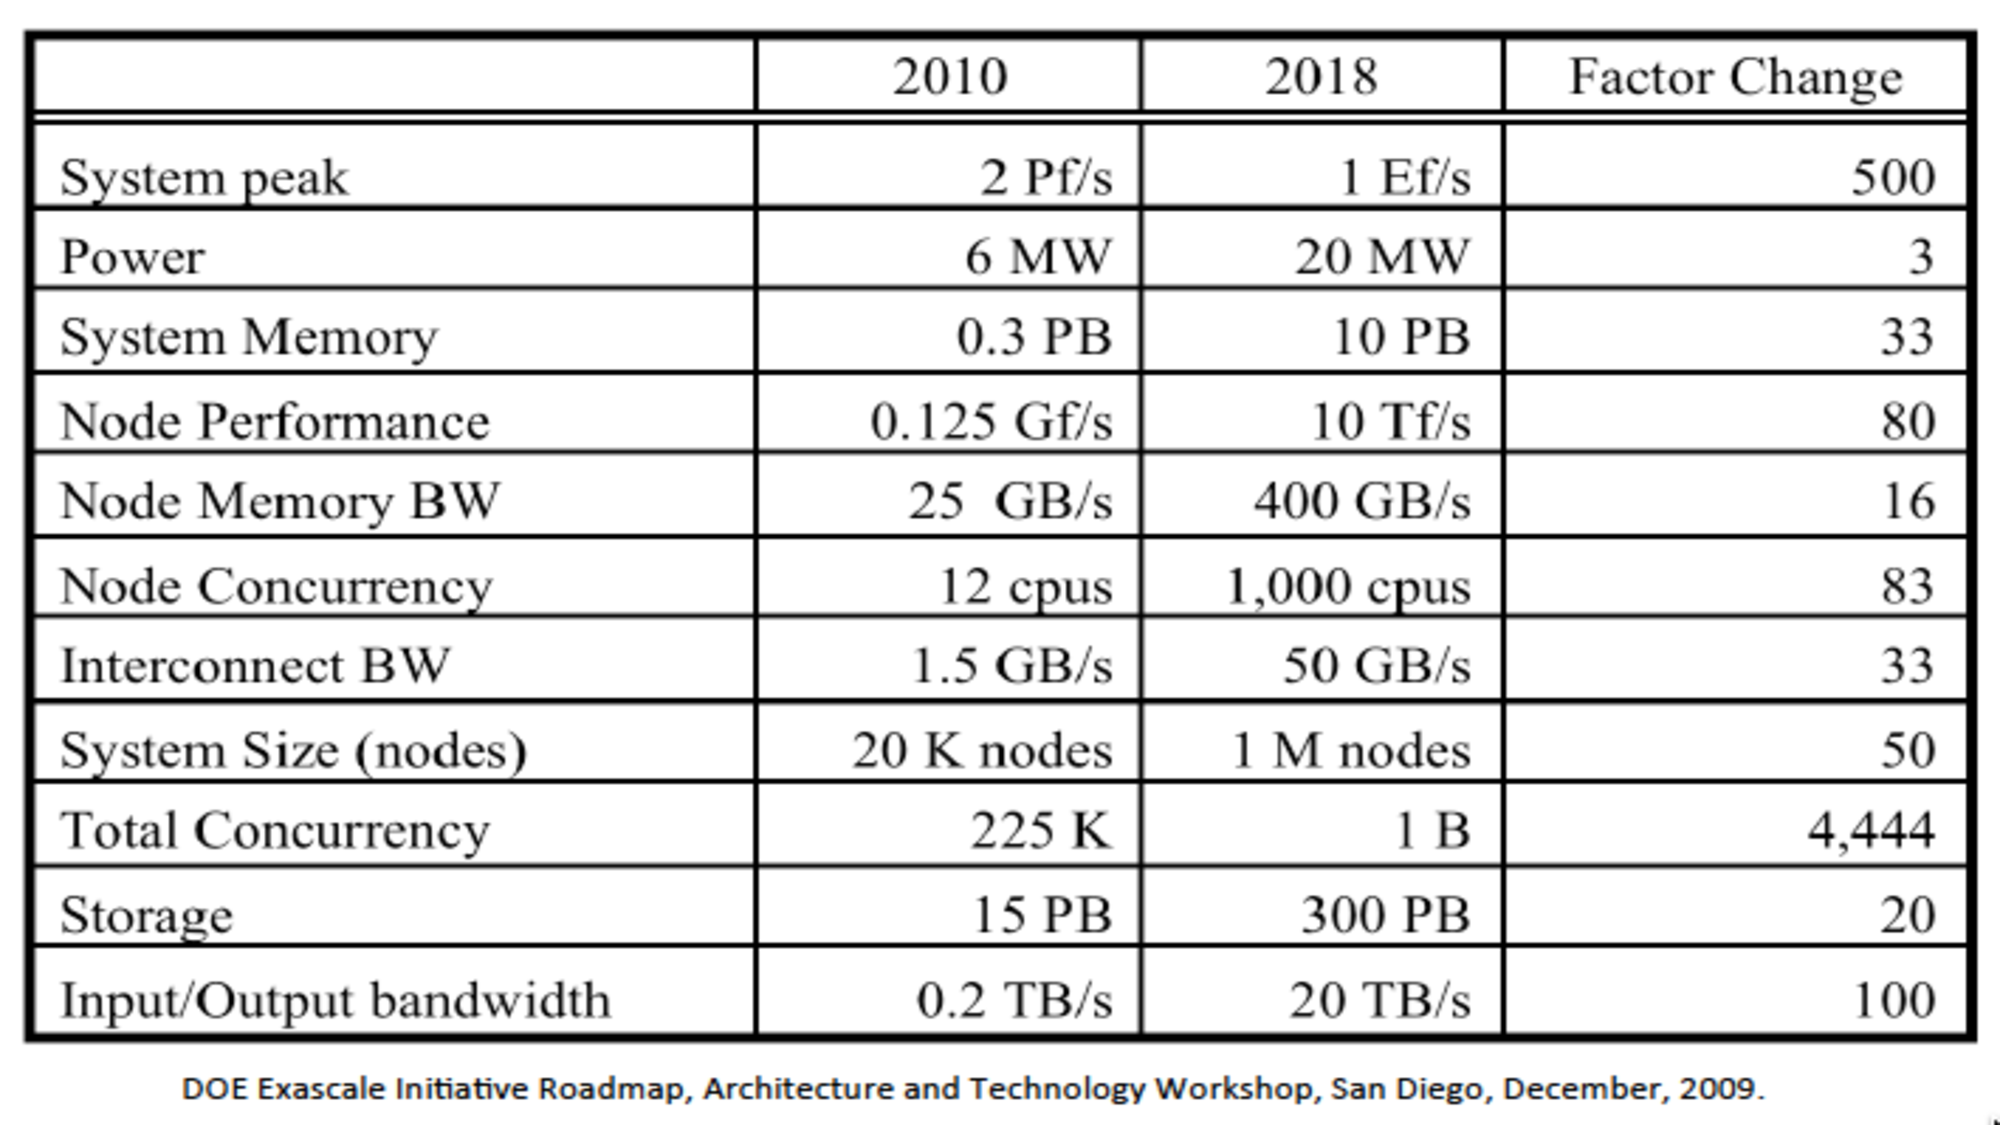
\includegraphics[width=0.85\textwidth]{chapter_1_figures/petascale_to_exascale_chart.pdf}
%    \caption{Concurrency trends in high performance computing
%      platforms.}
%    \label{fig:trends}
%\end{figure}

From the perspective of reproducibility of applications, the trade-off
between performance and determinism presents two distinct
challenges. First, permitting non-deterministic ordering of
interprocess communication opens the door to numerical
irreproducibility via the interaction between reduction order and the
non-associativity of floating-point arithmetic. This is
defined in this thesis as the numerical challenge.

Second, non-determinism significantly hampers debugging efforts during
application development and scaling. Specifically, there exist cases
where bugs manifest only during some executions due to a particular
ordering of message receives. If the application does not guarantee a
specific message receive order then this class of bugs becomes very
hard to diagnose and treat since the cost of reproducing them
significantly increases. Recent work by 
Sato \textit{et. al}~\cite{NINJA:Sato:2017}, 
presents a case-study of the impact of a
non-deterministic bug in terms of developer time and computational
resources. This is defined in this thesis as the debugging challenge.

% Factors that impacts non-determinism associated to the increase
% concurrency include overlapping communication and computation, network
% and configurations delays, and congestion and
% contention. Non-determinism can be internal or external: the first is
% when internal states of the system varies from run to run, and the
% second is when numerical outputs observed vary from run to run.
% Non-determinism is causing two major challenges for the scientific
% community: the numerical and debugging challenges. In numerical
% scenarios, non-determinism does not allow us to control variability
% thresholds (error) in computational results.  In debugging scenarios,
% non-determinism does not allow us to control the interactions among
% processes threads and isolate the causes of rare bugs in software.

\subsection{Overview of Numerical Challenge} 

Because floating-point numbers have finite precision, no simulation
can be completely free of error. As hardware resources grow, the
scientific computation taking advantage of that hardware has become
increasingly complex. A consequence of the scale of computation is
that even small errors at the beginning of the simulation may
eventually compound into significant accuracy problems, which may call
into question the validity of hours and hours of
computation. Multithreading complicates matters by introducing
nondeterminism. Not only do errors accumulate throughout a
computation, but a scientist may run the same computation several
times with differing results. According to a recent report from the
Department of Energy~\cite{Doe2014}, by the end of this decade the
level of concurrency of the supercomputing platforms on which
simulations are executed is expected to increase by a factor of at
least 4000.  The question that must be answered is: Can the scientific
community trust simulations executed on next-generation exascale
architectures?

In Chapter~\ref{chap2}, we assess the effectiveness of several mathematical
techniques to pursue reproducible accuracy on exascale platforms with
multithreading hardware consisting of multicore processors coupled
with many-core accelerators.  We refer to \textit{reproducibility} as
``closeness of agreement among repeated simulation results under the
same initial conditions'' and \textit{accuracy} as ``conformity of a
resulting value to an accepted standard, or scientific laws'' (from
Van Nostrand’s Scientific Encyclopedia). Rather than focusing on
bitwise reproducibility, we study methodologies to minimize the
propagation of errors and, thereby, limit their impact on the results
of a simulation, increasing both the reproducibility of the simulation
and the meaningfulness of the results. 

\subsection{Overview of the Debugging Challenge}

Application developers employ a variety of programming techniques to
maximize the scalability of their applications on the increasingly
concurrent platforms. In the case of message-passing applications, one
notable technique is the use of non-blocking point-to-point
communication, which permits communication and computation to be
overlapped, leading to an increase in scalability. The price paid
however, is the loss of determinism mentioned above. The program's
interprocess communication does not behave exactly the same way during
each execution. Figure~\ref{fig:example_nondeterminism} shows two high
level examples of non-deterministic executions when the same
destinations received the messages in different orders and when
messages are exchanged between two different destinations.
\begin{figure}[!htb]
    \centering
    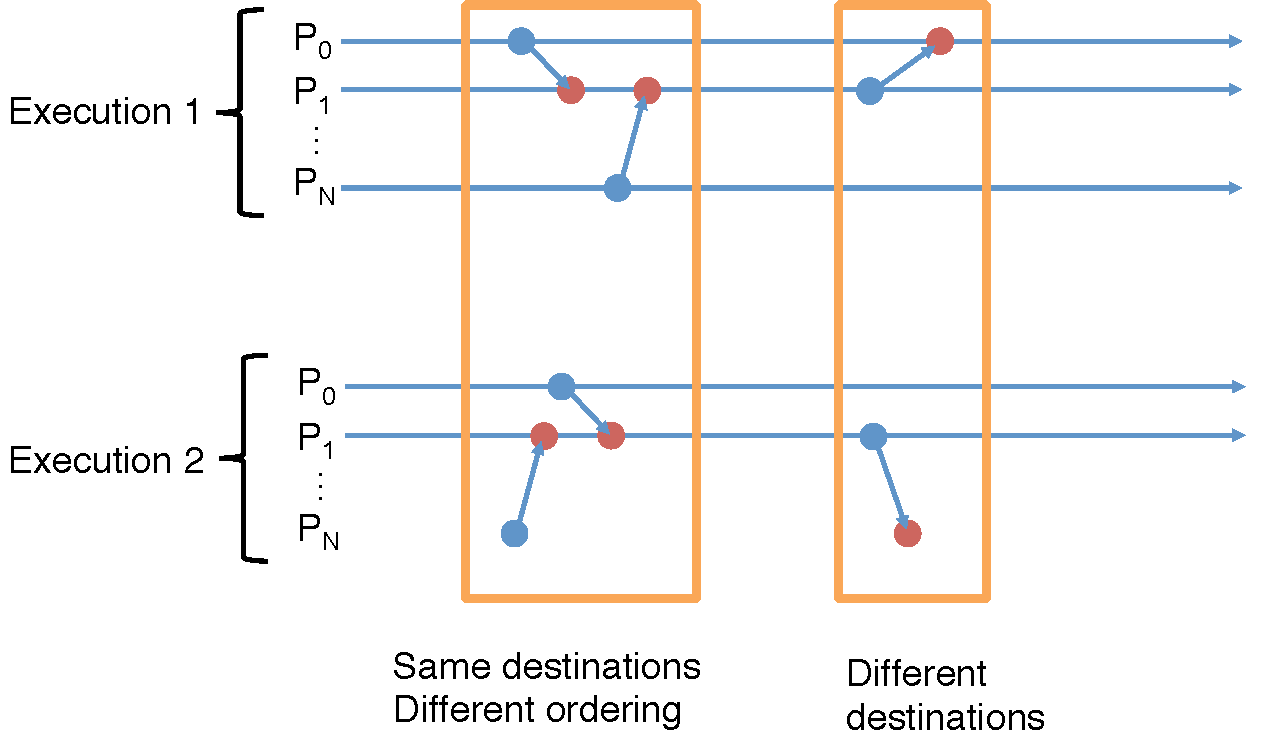
\includegraphics[width=0.85\textwidth]{chapter_1_figures/example_nondeterminism.pdf}
    \caption{Two examples of non-determinism associated to message
      passing executions.}
    \label{fig:example_nondeterminism}
\end{figure}
This problem is further exacerbated by use of wildcard receives (i.e.,
permitting a process to receive its next message from any available
sender, rather than a specific one). This non-determinism impedes
debugging efforts by vastly increasing the cost in computational resources
and developer time needed to reproduce bugs, necessitating the 
use of record-and-replay tools.
The question we address is: How can record-and-replay 
tools be improved so that they can continue to enable debugging on  
future exascale systems. 

In Chapter~\ref{chap3}, we assess the effectiveness of multiple logical
clock ticking policies, including a novel ticking policy we develop,
when used as the underlying ordering mechanism in
Clock-Delta Compression (CDC), a state-of-the-art record-and-replay technique. 
We evaluate ticking policies' effectiveness in enabling CDC's compression
against a real application in a diverse set of runtime conditions that 
reflect variability in floating-point workload and communication intensity 
that HPC applications exhibit. 

\section{Thesis Statement}
We claim that the massive increase in total system concurrency that will accompany 
exascale systems will significantly amplify the problems of numerical
irreproducibility and impededed debugging that HPC developers currently
face. We address the numerical challenge of reproducibility by illustrating
the pressing need for intelligent runtime selection of reduction operators 
for problematic floating-point inputs. We address the debugging challenge 
by demonstrating the pressing need for logical clock ticking policies that 
reduce then out-of-order message rate of the Clock-Delta Compression
record-and-replay technique. 

\section{Contributions}

When dealing with the numerical challenge, our contributions are as
follows:
\begin{itemize}
\item We evaluate and compare the reproducibility of four summation
  techniques applied to a simulated exascale environment.
\item We demonstrate that commonly accepted practices for predicting
  and mitigating errors offer incomplete characterizations of the
  reproducibility of numerical algorithms when applied in isolation.
\item We demonstrate the need for data-aware software to intelligently
  choose reduction algorithms to guarantee reproducibility without an
  unnecessary loss in performance.
\end{itemize}

When dealing with the debugging challenge, our contributions are as
follows:
\begin{itemize}
\item We propose a logical clock ticking policy based on floating-point
    operations that can be integrated in Clock-Delta Compression.
\item We provide a comparison of three ticking policies' 
    (basic Lamport clock ticking, wall-time-based ticking, and FLOPs-based ticking)
    effectiveness under diverse runtime conditions. 
\item We demonstrate the potential for extending logical clock ticking
    policies to adapt to applications' non-deterministic communication patterns.
\end{itemize}

\section{Thesis Outline}
Chapter~\ref{chap2} introduces our work on reproducible numerical
accuracy, and presents results on selection of compensated summation
algorithms based on mathematical properties of summands. Chapter~\ref{chap3}
introduces our work on record-and-replay tools, and presents results 
on our fine-grained logical clock ticking policy as applied to the
Clock-Delta Compression record-and-replay technique. Chapter~\ref{chap4}
lays out the plan for extending our research on reproducibility in HPC
by applying the lessons learned in Chapter~\ref{chap2} and Chapter~\ref{chap3}
to non-deterministic commmunication patterns extracted from applications. 
 
    % This file (chap1.tex) contains the text
                   % for Chapter 1.
                   
%
% This is Chapter 2 file (chap2.tex)
%
\chapter{The Numerical Challenge} \label{chap2}

\section{Introduction}

In this chapter we first summarize both well-known and emerging
sources of numerical inaccuracy and describe techniques for supporting
reproducible accuracy. We then prove the inadequacy of conventional
wisdom when dealing with this problem and provide strong evidence of
the need for intelligent reduction operations at the extreme scale
before to conclude the chapter with a short summary of our our learned
lessons.

\section{Sources of Numerical Inaccuracy}
%\label{sec:sources}

Achieving reproducible numerical accuracy at exascale faces two
fundamental roadblocks: nonassociativity of floating-point arithmetic
and nondeterminism in the order by which operands are reduced.  In
this section, we provide an overview of the challenges that arise when
nonassociativity collides with nondeterministic reduction. To that
end, we discuss the primary mechanisms by which floating-point error
arises and propagates. We also summarize the existing body of work
addressing issues of nondeterminism at exascale.

\subsection{Nonassociativity: A Consequence of Finite Precision}

Floating-point computations suffer loss of accuracy, compared with the
same expression's evaluation in exact arithmetic, through two primary
mechanisms: alignment error and subtractive cancellation.  Alignment
error, by far the most common error modality, results from summation
of values whose exponents differ. Alignment error is possible whenever
two floating-point numbers that differ in magnitude by at least a
factor of two are added~\cite{Castaldo}. The amount of information
about the smaller operand lost due to alignment error is related to
the disparity between the operands' magnitudes. The other mechanism is
subtractive cancellation, which occurs when very small values are
obtained from the addition of two values with similar magnitude and
opposite sign. Subtractive cancellation, in contrast to alignment
error, is not a source of error \emph{per se}, but a means by which
inaccuracy in low-order mantissa bits of operands is transferred to
high-order mantissa bits of their sum.

A consequence of these inaccuracies is the well-known fact that
floating-point arithmetic operations are nonassociative, so the order
in which floating-point numbers are reduced via an operator (e.g., +,
-, *, /) influences the result.  For example, let $a = 10^9$, $b =
-10^{9}$, and $c = 10^{-9}$. In infinite precision, the summation
orders $(a + (b + c))$ and $((a+b) +c)$ are equivalent, but even in
double-precision floating-point arithmetic, the two distinct summation
orders yield different values.
\begin{center}
	$((a + b) + c) = ((10^9 - 10^9) + 10^{-9}) = 10^{-9}$ \\
	$(a + (b + c)) = (10^9 + (-10^9 + 10^{-9})) = 0$ 
\end{center}
For a small example such as this one, the flaw is clear, namely, that
the small-magnitude value $c$ is ``absorbed" by the much larger value
$b$.

\subsection{High Concurrency: A Consequence of Extreme Scale}

Contemporary petascale platforms consist of up to millions of
processor cores that must act in concert to effect large
simulations. Even at these scales, the cost of achieving not only
accuracy in floating-point reductions but reproducible accuracy is
felt. The scientific community at large has set its sights on
deployment of an exascale computing platform, and in response the HPC
community has identified a canonical set of challenges to implementing
an exascale machine~\cite{Doe2014}. Although emerging developments in
low-power hardware, advanced systems software, and algorithm design
show promise, it has become increasingly evident that achieving
reproducible numerical accuracy at exascale cannot rely on
deterministic reduction. Exascale computations will simply have to
weather perturbations in their reduction trees through algorithmic
means. In this section, we summarize key results demonstrating how
variability in reduction trees induces variability in sums of
floating-point numbers. Additionally, we present a set of findings,
commentary, and expert recommendations supporting our claim that
deterministic reduction trees at exascale will be unfeasible.

Throughout this section and the remainder of the chapter, we adopt the
view of a concurrent sum of floating-point numbers at the extreme
scale as a \emph{reduction tree}, which we define as a full binary
tree whose $N$ leaf nodes correspond to floating-point operands and
whose internal nodes correspond to the partial reductions formed in
the process of computing the final result--the root node.  Reduction
trees can vary in two ways: shape and assignment of operands to
leaves. When we refer to the shape of a reduction tree, we mean the
particular way in which nodes are linked by
edges. Figure~\ref{fig:redtree_diffshape} shows two differently shaped
reduction trees: a balanced (parallel) reduction tree and an
unbalanced (serial) reduction tree. For a fixed set of operands, even
two reduction trees with the same shape can yield different values for
the reduction if the assignment of operands to leaves differ between
the two trees.
\begin{figure}[!htb]
% \label{fig:redtree_diffshape}
\centering
%\minipage[t]{0.45\textwidth}
%\begin{tabular}{c}
\subfigure[A balanced (parallel) reduction tree]{
%{.5\textwidth}
\centering
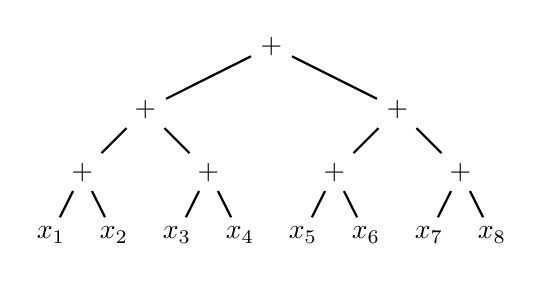
\begin{tikzpicture}[scale=0.8]
	\node at (0, 0) (1) {$x_1$};
	\node at (1, 0) (2) {$x_2$};
	\node at (2, 0) (3) {$x_3$};
	\node at (3, 0) (4) {$x_4$};
	\node at (4, 0) (5) {$x_5$};
	\node at (5, 0) (6) {$x_6$};
	\node at (6, 0) (7) {$x_7$};
	\node at (7, 0) (8) {$x_8$};
	\node at (.5, 1) (11) {$+$};
	\node at (2.5, 1) (12) {$+$};
	\node at (4.5, 1) (13) {$+$};
	\node at (6.5, 1) (14) {$+$};
	\node at (1.5, 2) (21) {$+$};
	\node at (5.5, 2) (22) {$+$};
	\node at (3.5, 3) (top) {$+$};
	\draw [draw=black, thick] (1)--(11)--(2);
	\draw [draw=black, thick] (3)--(12)--(4);
	\draw [draw=black, thick] (5)--(13)--(6);
	\draw [draw=black, thick] (7)--(14)--(8);
	\draw [draw=black, thick] (11)--(21)--(12);
	\draw [draw=black, thick] (13)--(22)--(14);
	\draw [draw=black, thick] (21)--(top)--(22);
\end{tikzpicture}
\label{redtree_balanced}}
\subfigure[An unbalanced (serial) reduction tree]{
\centering
	\begin{tikzpicture}[scale=0.8]
	\node at (-2, 0) (empty) { };
	\node at ( 4, 0) (empty) { };
	\node at (0, 0) (1) {$x_1$};
	\node at (1, 0) (2) {$x_2$};
	\node at (.5, 1) (11) {$+$};
	\node at (1.5, 1) (12) {$x_3$};
	\node at (1, 2) (21) {$+$};
	\node at (2, 2) (22) {$x_4$};
	\node at (1.5, 3) (31) {$+$};
	%\node at (2.5, 3) (32) {$x_5$};
	%\node at (2, 4) (41) {$+$};
	%\node at (3, 4) (42) {$x_6$};
	%\node at (2.5, 5) (51) {$+$};
	%\node at (3.5, 5) (52) {$x_7$};
	%\node at (3, 6) (61) {$+$};
	%\node at (4, 6) (62) {$x_8$};
	%\node at (3.5, 7) (top) {$+$};
	\draw [draw=black, thick] (1)--(11)--(2);
	\draw [draw=black, thick] (11)--(21)--(12);
	\draw [draw=black, thick] (21)--(31)--(22);
	%\draw [draw=black, thick] (31)--(41)--(32);
	%\draw [draw=black, thick] (41)--(51)--(42);
	%\draw [draw=black, thick] (51)--(61)--(52);
	%\draw [draw=black, thick] (61)--(top)--(62);
	\end{tikzpicture}
\label{redtree_unbalanced}}
\caption{Two reduction trees at the opposite ends of the spectrum.}
\label{fig:redtree_diffshape}
\end{figure}

The effect of varying reduction tree shape and varying operand-to-leaf
assignment is explored in~\cite{chiang13}. In their work, a set of
eight identical floating-point values is summed via three differently
shaped reduction trees, yielding in each case a different value for
the sum. Another set of eight floating-point values, six small and two
large, is summed via three reduction trees of the same shape, but with
different assignments of summands to leaves. Again, all three computed
sums disagreed.  One key observation is that the consequences of
nondeterministic reduction and floating-point nonassociativity are
felt even for extremely small examples.

On exascale systems the high level of concurrency will not allow the
user to enforce any specific reduction order because doing so is
either too expensive or impossible. At the same time variability in
floating-point error accumulation may become so great that debugging
is impaired or, worse, fundamentally incorrect results are
accepted. An exascale algorithm must exploit the extreme level of
concurrency, minimize communication (for speed and power reduction),
tolerate frequent hardware failures, and utilize resources as they
become available~\cite{Doe2014}, all the while providing some trust in
the computation's result.

The conflict between achieving reproducible accuracy and achieving
performance is primarily due to the fact that even on current HPC
platforms, communication costs dominate arithmetic costs.  Simply put,
the most performant reduction trees are those that take into account
the underlying physical topology of the system, which means reducing
values in an order based on which core produced them, not necessarily
their arithmetical properties. Conversely, the reduction trees that
result in the least error accumulation reduce values based on their
arithmetical properties, not their position in the topology of the
system. Recently, Balaji and Kimpe~\cite{balaji13} showed not only
that topology-aware reduction trees for MPI collective operations
outperform fixed-reduction trees but that the performance advantage of
allowing the reduction tree to conform to the system topology, as
opposed to a specified ordering of partial reduction, increases with
the number of cores.

\section{Mathematical Techniques}
%\label{sec:techniques}

In response to the challenges posed by the nonassociativity of
floating-point summation and the nondeterminism at the extreme scale,
mathematical techniques can be applied to mitigate the degree to which
computed sums exhibit sensitivity to reduction order. Lower
sensitivity results in increasingly reproducible results.  Techniques
can range from simple fixed-reduction orders to more sophisticated
prerounded algorithms. In this section we provide a general overview
of the techniques; however, in the rest of the chapter, we consider only
the compensated summation algorithms (Kahan and composite precision)
as well as the prerounded algorithms for our studies because they are
the only methods that can be feasibly applied at the exascale.

\subsection{Fixed-Reduction Order}

To apply fixed-reduction order, we need to ensure that all
floating-point operations are evaluated in the same order from run to
run. Two major problems exist for this strategy. The obvious problem
is that ensuring that the reduction proceeds according to a
user-determined reduction tree incurs massive communication and
synchronization costs.  Additionally, determining exactly which
reduction tree achieves minimal error for a given set of summands is
nontrivial. Conventional wisdom suggests summing the values in
ascending order if they all have the same sign, and in descending
order of magnitude if they are not. The first case is rare, however,
and the second case assumes that no error beyond initial
representation error is present in the summands; otherwise it is far
more vulnerable to catastrophic cancellation.  In summary, fixing the
reduction order is difficult to do correctly where it is possible, but
the salient point is that it cannot be done in a cost-effective way at
exascale~\cite{Demmel_Hida}.

\subsection{Interval Arithmetic}

Techniques based on interval arithmetic replace floating-point types
with custom types representing finite-length intervals of real
numbers. The actual value of the reduction is guaranteed to lie within
the interval. The width of the interval increases with the uncertainty
of the computation. While the techniques are reproducible by design,
they also cause large slowdown and are not suitable for applications
needing many digits of accuracy.

\subsection{High-Precision Arithmetic}

Perhaps the most obvious technique, and certainly the most popular in
real applications, is to use higher-precision floating-point types. To
our knowledge, the earliest work directly addressing the issue of
numerical reproducibility~\cite{he} demonstrates the use of the
double-double precision floating-point type in a critical section of
code to curtail variability in a global sum. In that work, the goal of
using multiple floating-point types was explicitly to achieve
reproducible results. Parallel to that effort, significant progress
has been made in the field of automated floating-point precision
tuning (e.g., ~\cite{precimonious}). Precision tuning is an attempt
to reduce precision where possible while maintaining a prescribed
degree of accuracy.  While one can achieve greater
reproducibility by pursuing greater accuracy, the use of
high-precision arithmetic can result in memory-demanding
algorithms. By increasing the size of floating-point variables in most
numerically sensitive parts of the algorithm, for example with manual
changes made by an expert or by some form of analysis, we can reduce
the memory requirements. Still the technique relies on either human
experts or other software and thus is probably unsuitable for many 
of the use cases discussed in the recent DOE exascale
report~\cite{Doe2014}.

\subsection{Compensated Summation Algorithms}

To compute the sum of $n$ values, we obtain $n-1$ partial sums in the
process. For each of these partial sums, the magnitude of error can be
estimated.  Based on that estimate, an attempt can be made to
compensate for that error by adding an error term to each partial
sum. Compensated summation is a relatively old technique, having been
introduced by Kahan in~\cite{kahan65}; but families of more
sophisticated compensated summation algorithms have been developed,
such as composite precision (CP) summation~\cite{Taufer2010}. In
Kahan's algorithm the estimated error is added back into the sum at
each step. In CP, the error summation is kept and propagated as each
of the summations are performed and added back in only at the end.

\subsection{Prerounded Summation Algorithms}

More recently, an approach called prerounded summation has emerged for
reproducible and accurate summation.  The common strategy used by this
type of algorithm is splitting the operands into ``high-order" and
``low-order" parts with the property that the high-order parts can be
summed irrespective of summation order and the low-order parts can be
neglected, or recursed upon, for higher accuracy. The algorithms
proposed by Demmel and his group are integrated into the ReproBLAS
library~\cite{demmel}, which at this time is undergoing active
development.

\section{Inadequacy of Conventional Wisdom}

The management of reproducible numerical accuracy is closely related
to the task of estimating and predicting error accumulation.  Three
common approaches exist, typically used in isolation, to quantify and
mitigate error accumulation. Two of the approaches can be broadly
classified as techniques for error estimation: using worst-case error
bounds and attempting to track or avoid subtractive cancellation. The
third approach is the use of summation algorithms that are believed to
be inherently less sensitive to variability in the reduction tree.  We
emphasize that these approaches have significant value. However, we
demonstrate that the use of any one approach, in isolation, will not
guarantee the reproducibility desired without a potentially
significant loss of performance.

\subsection{Using Analytical Error Bounds}

The analysis of the error for a single floating-point sum can be
extended to produce a worst-case error bound for the reduction of
multiple floating-point values.  For IEEE-compliant implementations of
floating-point arithmetic, we have the following bound on the roundoff
error for a single operation. Let $x, y$ be floating-point numbers,
let $\texttt{fl}(x+y)$ be their rounded sum according to a given
rounding rule, and let $(x+y)$ be their exact sum:
\begin{center}
	$\texttt{fl}(x+y) = (x+y)\cdot (1+\delta)$ 
\end{center}
where $|\delta| \leq u$ where $u$ is the unit-roundoff and may be
written $u = \frac{1}{2}\beta^{1-p}$, where $\beta$ is the base and
$p$ is the number of mantissa bits of the representation of $x$ and
$y$. Equivalently, if we let $z$ denote the exact sum $x+y$, we obtain
a bound on the absolute error $| \texttt{fl}(x+y) - z| \leq u$.  With
some algebra, one can prove an upper bound on the error in a sum of
$n$ floating-point numbers. We do not include the proof here (it may
be found in~\cite{Higham93}), but we state the result. Let $x_1,
\ldots, x_n$ be floating-point numbers, let $z$ denote their exact
sum, and let $\sum\limits_{i=1}^{n}x_i$ denote their sum in
floating-point arithmetic. Then we have the following upper bound on
the absolute error in the sum:
\begin{center}
	$|\sum\limits_{i=1}^{n}x_i - z| < n \cdot u \cdot \sum\limits_{i=1}^{n} |x_i|.$
\end{center}

%While this upper bound is useful in the sense that it is better than
%nothing, it is excessively loose in practice.  We present the
%analysis for a single sum, the extension to a sum of $N$ values, and
%data demonstrating the looseness of the bound.  Unlike arithmetic
%over the real numbers, arithmetic with floating-point operands
%suffers from some limitations. Due to the availability of a finite
%number of bits to represent each number, the vast majority of real
%numbers do not have an exact representation in a given system of
%floating-point arithmetic. Consequently, when two floating point
%values are summed, the result must often be rounded according to some
%rounding rule. The difference between this rounded result and the
%exact result had the summation been conducted over the real numbers
%is what we refer to as roundoff error.  In practice however, we are
%more interested in bounds on the error that accumulates over the
%course of summing $n$ floating-point values.

Using analytical or statistical worst-case error bounds causes
overestimation of the errors. Figure~\ref{fig:errorbounds} shows an
empirical case study in which we measure the error magnitudes for
$10,000$ values sampled in the range $(-1000, +1000)$ and summed by
using $10,000$ different summation orders.
\begin{figure}[!htb]
  \centering
  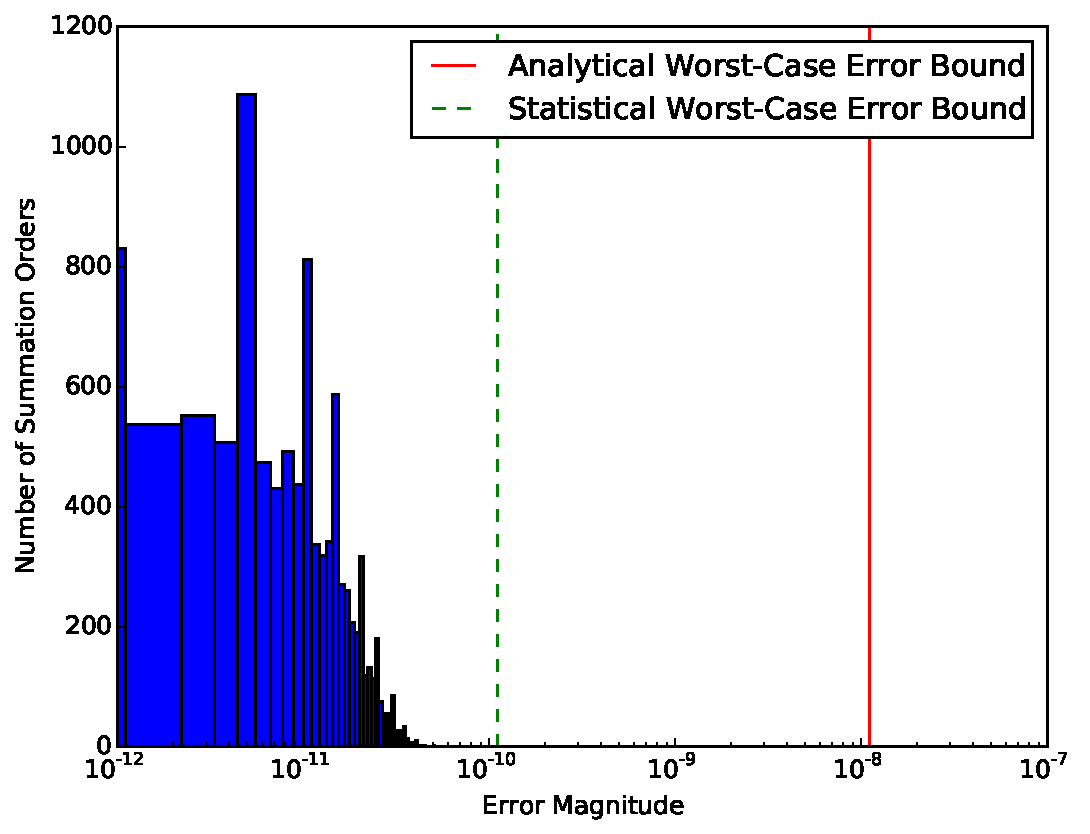
\includegraphics[width=0.80\textwidth]{chapter_2_figures/error_variability_histogram.pdf}
  \caption{Empirical study of error magnitudes and worst-case error
    bounds for $10,000$ summations of $10,000$ values randomly
    sorted.}
  \label{fig:errorbounds}
\end{figure}
The figure also shows both the analytical and statistical worst-case
error bounds. Both error bounds significantly overestimate the error
magnitude. At the same time we observe the large range of measured
errors obtained for the same set of values just by randomly shuffling
the order in which the terms are summed.

\subsection{Tracking Cancellations}

When considering sets of summands with both positive and negative
values, the potential for \emph{catastrophic cancellation} arises in
the computation of the sum. This numerical phenomenon can result in
large relative errors in both the partial and final sums, leading to
the intuitively appealing perspective of achieving reproducible
accuracy by structuring reductions to avoid cancellation.

Cancellation in general refers to the scenario where the sum of two
floating-point values has a smaller exponent than both of the
summands. In order to subtract one floating-point number from another,
their binary points are aligned and the mantissa of their difference
is determined by subtracting the mantissas of the operands bitwise and
then \emph{renormalizing} the result. The effect of the
renormalization process is that the lower-order bits of the operands
determine the higher-order bits of the result. If both summands are
exact in the sense that their mantissa bits are not carrying the error
from previous computations---as is almost never the case---then their
difference can be considered accurate. However, if the low-order bits
of the operands are inaccurate due to alignment error, many or all of
the mantissa bits of the difference of the operands may be
inaccurate. This is the ``catastrophic" case.

We emphasize, however, that cancellation does not in and of itself
cause error to accumulate. Rather, it reveals error that has already
accumulated in the operands. In a sense, relative error can increase
because of catastrophic cancellation as uncertainty in
less-significant bits of the operands' mantissas is transferred to
uncertainty in the most significant bits of the result's
mantissa. Nevertheless, the number of cancellations is not a reliable
indicator of the overall problem.

To prove this claim, we generate a counterexample with a set of
$1,000$ floating-point numbers uniformly distributed in $[-1, 1]$.  We
compute the sum of these numbers using 100 distinct summation orders
and determine the error for each order. We assess cancellation for
each order using the numerical library CADNA~\cite{jezequel}. CADNA
uses the CESTAC method to identify instances of cancellation in a sum
and, for each instance, estimate the difference between the number of
accurate digits in the operands and the number of accurate digits in
the result. In this sense, a cancellation resulting in the loss of
four digits of accuracy is more severe than a cancellation resulting
in the loss of only two digits. Figure~\ref{fig:errorcancellations}
shows the cancellation counts and error magnitudes for several
summation orders of the set of interest for our counterexample. Each
summation order is represented by five bars, four showing the number
of cancellations resulting in the loss of one, two, four, and eight
digits, respectively, and a fifth bar showing the error magnitude,
scaled for ease of viewing. We observe that the number of
cancellations, at any of the considered severities, does not
consistently predict error magnitude.  In particular, consider
summation orders 2 and 4. Order 2 has about 5X as many digit
cancellations as order 4, but only half the error. This result lends
credence to the view that although it is tempting to view ``keeping
track of cancellations" as a valid strategy for managing error and
ensuring reproducibility, there is not a simple correspondence between
instances of cancellation and error magnitude. Rather, the
relationship between cancellation and error depends on knowledge of
how much error has already accumulated in the operands involved in the
cancellation, a quantity whose estimation is impeded by the previously
discussed loose error bound.
\begin{figure}[!htb]
  \centering
  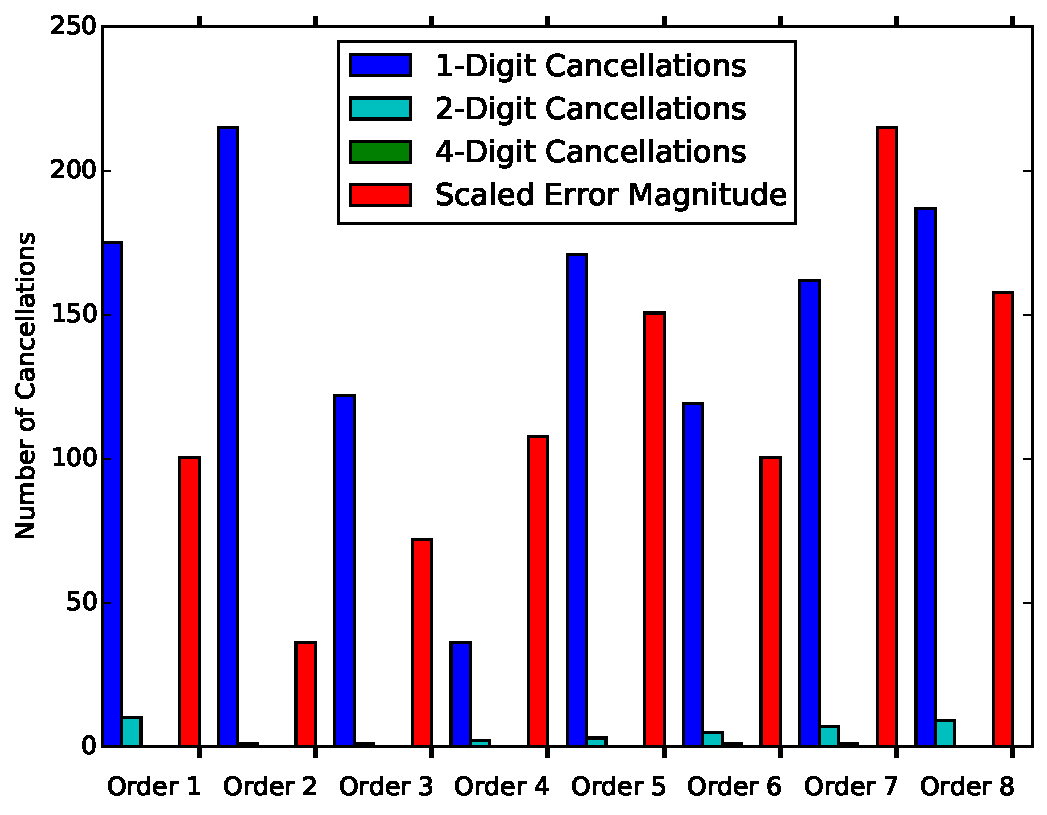
\includegraphics[width=0.80\textwidth]{chapter_2_figures/cancel_chart.pdf}
  \caption{Empirical study of cancellations vs. error magnitude
    for different summation orders.}
  \label{fig:errorcancellations}
\end{figure}

\subsection{Choice of Summation Algorithm}

Apart from the standard iterative summation algorithm, we examine
other summation algorithms that exhibit reduced sensitivity to
variability in the reduction tree. However, each of these algorithms
incurs a certain performance penalty relative to the standard
summation. Standard summation is the cheapest and least
complex. Kahan's compensated summation, then composite precision
summation, and finally prerounded summation are expected to
progressively provide more accuracy at the expense of performance. To
assess this performance impact, we measure the execution times of a
case study designed to emulate scenarios in scientific computing in
which partial data is locally generated on multiple processes and then
is globally reduced across the processes. Specifically, on each
process, we generate a chunk of a vector of values of length $10^6$
from a series that is known to sum to zero under exact arithmetic. We
locally reduce these values using each of the four summation
algorithms: in the case of Kahan and composite precision, we use the
summation operators in~\cite{Robey2011} and in the case of prerounded
summation, we use the dIAddd operator provided
in~\cite{reproblas}. Finally, we globally reduce the local sums by
using MPI\_Reduce with custom reduction operators for Kahan, composite
precision, and prerounded summations. To avoid time variations due to
network contention we run our tests on a single dedicated 48-core AMD
node. Each tests is repeated 20 times with a warmed
cache. Figure~\ref{fig:compare_runtimes} shows the average execution
times and Figure~\ref{fig:compare_ratios} shows the performance
penalties associated with more-reproducible summation. The latter
figure confirms the proposed ranking of the summation algorithms in
terms of performance expense.
\begin{figure}[!htb]
    \centering
    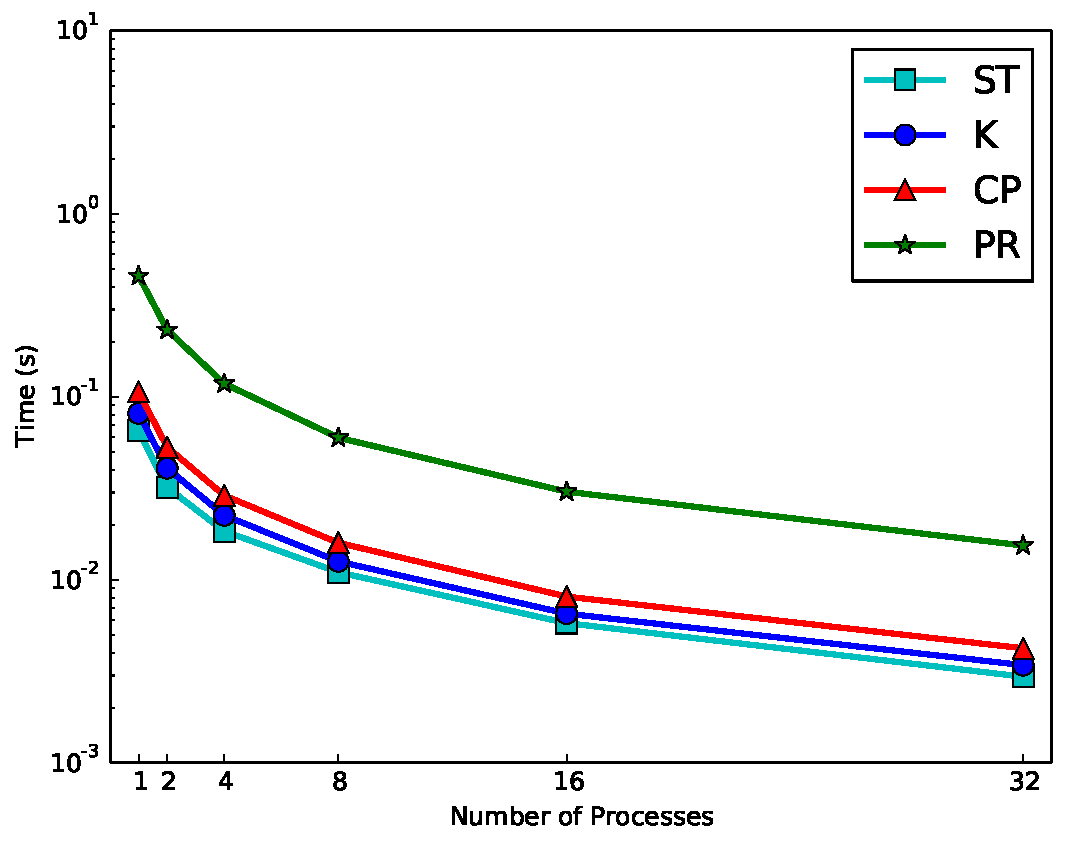
\includegraphics[width=0.80\textwidth]{chapter_2_figures/runtimes.pdf}
    \caption{Comparison of execution time to sum $10^6$ terms for
      standard summation (ST), Kahan's compensated summation (K),
      composite precision summation (CP), and prerounded summation
      (PR).}
    \label{fig:compare_runtimes}
\end{figure}
\begin{figure}[!htb]
    \centering
    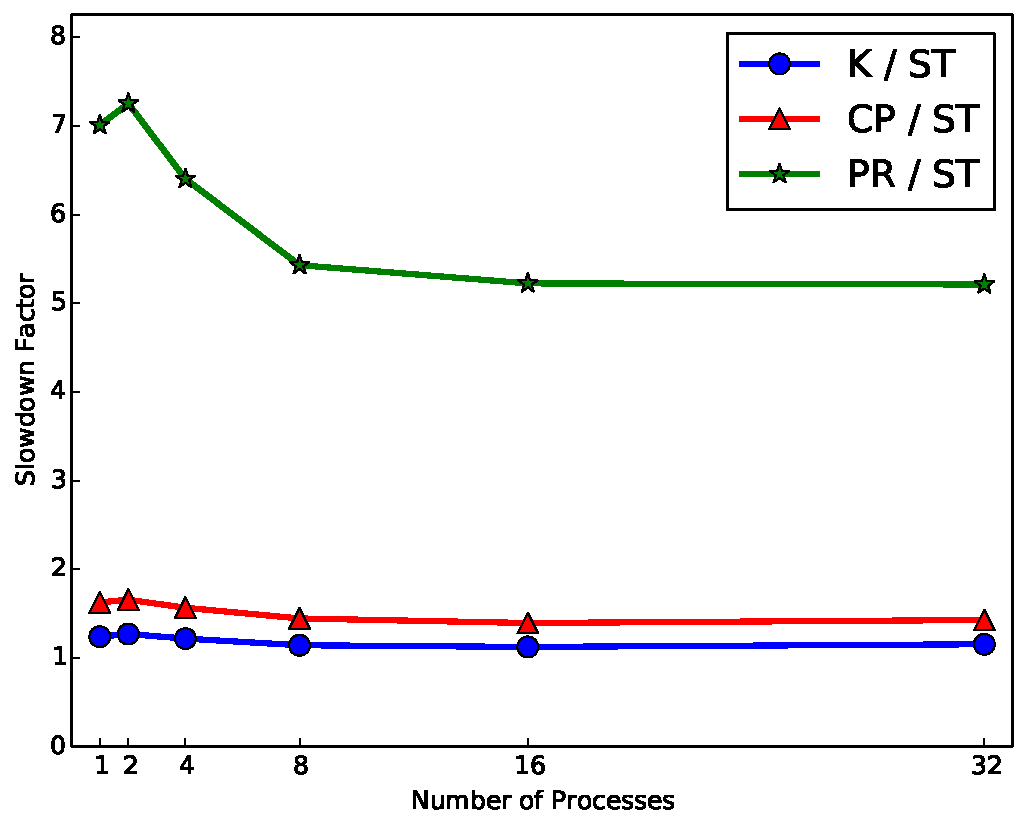
\includegraphics[width=0.80\textwidth]{chapter_2_figures/ratios.pdf}
    \caption{Performance losses of Kahan's compensated summation (K),
      composite precision (CP), and prerounded (PR) summations
      compared to the standard summation (ST).}
    \label{fig:compare_ratios}
\end{figure}

%Empirical results obtained on a single 48-core AMD node
%of a dedicated cluster support this characterization. Specifically,
%performance analysis of the four algorithms indicates that the
%execution time needed to reduce a vector $10^6$ elements increases
%with the reproducible accuracy provided by the algorithm as shown in
%Figure~\ref{fig:compare_runtimes}. Figure~\ref{fig:compare_ratios}
%shows the performance losses of the enhanced sums (i.e., Kahan's
%compensated summation, composite precision summation, and prerounded
%summation) which agree with previous empirical
%results~\cite{demmel}~\cite{Taufer2010}.

We argue that applying a judicious mixture of these algorithms, as
opposed to uniformly applying a single technique, is necessary for
achieving numerical reproducibility to the degree required by an
application, for a cost acceptable for that application.
Figures~\ref{fig:avgalgorithms}(a) and~\ref{fig:avgalgorithms}(b)
support this claim by showing the relative sensitivity of the three
summation algorithms: Kahan's compensated summation (K), composite
precision summation (CP), and prerounded summation (PR).  For a fixed
set of data we generate multiple reduction trees of the same shape but
with different assignments of operands to leaves. We construct the set
of summands to have mathematical properties that render its reduction
especially prone to both alignment error and loss of accuracy due to
cancellation. For each reduction tree, we compute the sum using each
of the four algorithms. By plotting the error magnitude, we see that
as a progressively greater amount of computation is invested in
compensating for roundoff error, the sum becomes less sensitive to the
varying reduction tree.
\begin{figure}[!htb]
\centering
\minipage[t]{0.40\textwidth}
\begin{tabular}{c}
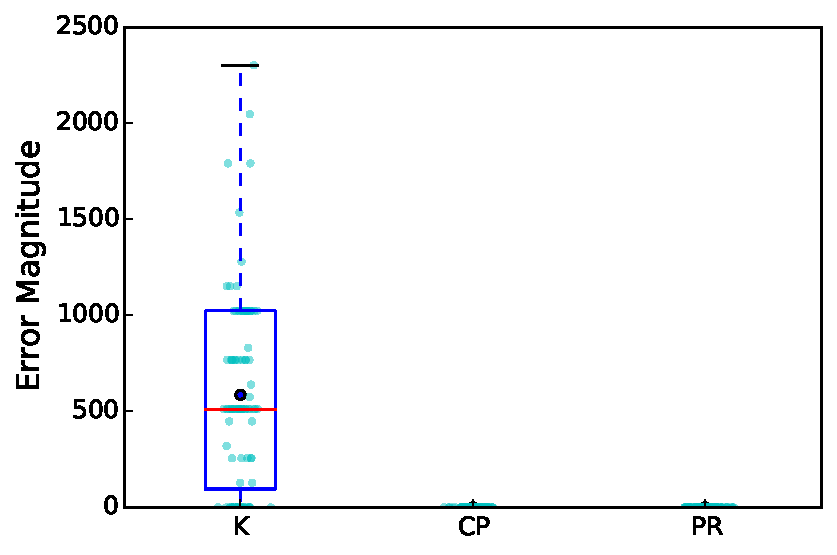
\includegraphics[width=\textwidth, height=8cm]{chapter_2_figures/draft_boxplot_alt_balanced_N=1048576.pdf} \\ 
(a) \\
\end{tabular}
\endminipage
\minipage[t]{0.30\textwidth}
\begin{tabular}{c}
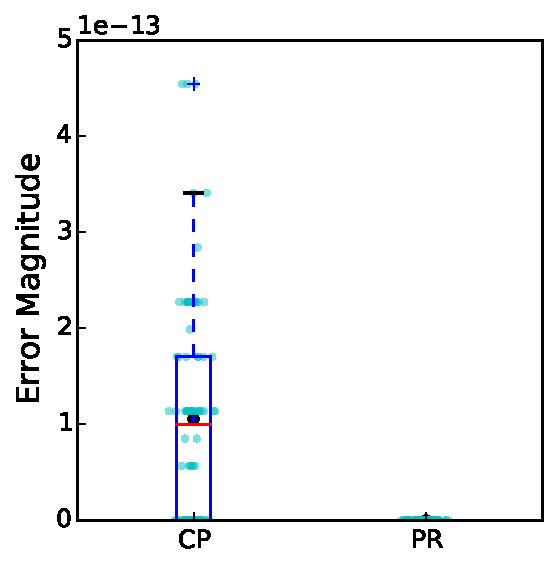
\includegraphics[width=\textwidth, height=8cm]{chapter_2_figures/draft_boxplot_balanced_cp_vs_preround_N=1048576.pdf}
\\ (b) \\
\end{tabular}
\endminipage
\caption{Empirical study of relative sensitivity of three summation
  algorithms: Kahan's compensated summation (K), composite precision
  summation (CP), and prerounded summation (PR). Note that (a) zooms
  into (b). }
\label{fig:avgalgorithms}
\end{figure}

\section{Exploring the Reproducibility Space} 

Previous work~\cite{chiang13, balaji13} found that reduction tree
shape and assignment of operands to its leaves (or threads) can have a
profound effect on the concurrent sum of $n$ floating-point numbers,
even when the operands themselves are subject to minimal alignment
error and have the same sign avoiding cancellation.  We build the work
in this chapter on this previous work by targeting a much larger
reduction scale and investigating the impact of four independent
parameters on the variability of a sum when the reduction order is
non-deterministic. The four parameters we consider are the condition
number, the dynamic range, the level of concurrency, and the reduction
algorithm. We present three kinds of results. First, we examine the
sensitivity to variations in the reduction tree of four summation
algorithms at increasing levels of concurrency. Second, we study the
impact of concurrency, condition number, and dynamic range on
reproducible numerical accuracy. Third, we provide evidence of the
need for selecting application-aware reduction algorithms.

\subsection{Experimental Environment and Parameters}

Building on the results of small nondeterministic reduction trees
established in~\cite{chiang13, langlois}, we consider reduction trees
at the size expected for exascale systems consisting of floating-point
operands reflective of those actually reduced in simulations. Since an
exascale system is not available, we emulate the reduction process
with $n$ threads, each computing one of the $n$ partial sums.  We
consider two tree shapes at opposite ends of the spectrum: a
completely balanced (see Figure~\ref{redtree_balanced}) tree and a
completely unbalanced (see Figure~\ref{redtree_unbalanced}) tree.  For
each tree shape, we generate distinct reduction trees by randomly
assigning operands to leaves. We also focus on sets of floating-point
summands whose mathematical properties are less amenable to
reproducible summation. We characterize sets of floating-point values
by their sum condition number and dynamic range. These are intrinsic
properties of the set of values; they are independent of any imposed
ordering. For a set of floating-point numbers $\{x_1, \ldots, x_n
\}$, the sum condition number is defined as
\[k = \left(\sum_{i=1}^{n}|x_i|\right)/\left|\sum_{i=1}^{n}x_i\right|\] and
the dynamic range is defined as
\begin{center}
	$dr = \texttt{exp}(\texttt{max}(|x_i|))-\texttt{exp}(\texttt{min}(|x_i|)),$
\end{center}
where $exp(x)$ is the value of the exponent in the representation of
$x$.  If the dynamic range of two numbers is larger than zero, then
alignment error will occur. For this reason, we use the dynamic range
of a set of values as a rough estimator of alignment error.  The
condition number does not correspond to a single mechanism by which
error accumulates.  Instead, it describes how sensitive the final sum
is to small errors in the partial sums.

Table~\ref{tab:parameters} shows small sample sets of values
presenting dynamic range $dr$ equal to 0, 8, and 16 as well as
condition number $k$ equal to 1, 1000, and $\infty$.  Note that $dr$
equal to $0$ means ``all exponents are the same'' and not that the
numbers are large or small; on the other hand a larger $dr$, for
example 8 or 16, means that a larger discrepancy exists between the
largest and smallest exponents. In other words, the sign on the
summands makes no difference, and the sum of summands makes no
difference. A condition number equal to 1 means ``all values in sum
have the same sign,'' while a condition number number infinity means
``the sum of all the values is 0.''
\begin{table}[!ht]
\caption{Example of sample set of values with specified dynamic range,
  $dr$, and condition number, $k$.}
\label{tab:parameters}
\center
\small
\begin{tabular}{|c|c|c|}
  \hline
  Sample Set of Values & $dr$ & $k$ \\
  \hline
  $\{$1.23e+32, 1.35e+32, 2.37e+32, 3.54e+32$\}$ & $0$ & $1$ \\
  $\{$1.23e-32, 1.35e-32, 2.37e-32, 3.54e-32$\}$ & $0$ & $1$ \\
  $\{$-1.23e+16, -1.35e+16, -2.37e+16,-3.54e+16$\}$ & $0$ & $1$ \\
  $\{$2.37e+16, 3.41e+8, 4.32e+8, 8.14e+16$\}$ & $8$ & $1$ \\
  $\{$3.14e+32, 1.59e+16, 2.65e+18, 3.58e+24$\}$ & $16$ & $1$ \\
  \hline
  $\{$2.505e+2, 2.5e+2, -2.495e+2, -2.5e+2$\}$ & $0$ & $1000$ \\
  $\{$5.00e+2, 4.99999e-1, 1.0e-6, -4.995e+2$\}$ & $8$ & $1000$ \\
  $\{$5.00e+2, 4.99...99e-1, 1.0e-14, -4.995e+2$\}$ & $16$ & $1000$ \\
  \hline
  $\{$3.14e+8, 1.59e+8, -3.14e+8, -1.59e+8$\}$ & $0$ & $\infty$ \\
  $\{$3.14e+4, 1.59e-4, -3.14e+4, -1.59e-4$\}$ & $8$ & $\infty$ \\
  $\{$3.14e+8, 1.59e-8, -3.14e+8, -1.59e-8$\}$ & $16$ & $\infty$ \\
  \hline
\end{tabular}
\end{table}
\normalsize In~\cite{chiang13} the operands are well-conditioned; they
have $k=1$ (the best possible condition number) and, when varying tree
shape, have $dr=0$. We instead focus on ill-conditioned inputs with
high dynamic range because reality is not so rosy. For example,
$N$-body simulations~\cite{bailey} involve reductions of
floating-point values that are ill-conditioned; both $k$ and $dr$ can
frequently be very large.

\subsection{Sensitivity of Summation Algorithms}

To examine the sensitivity of summation algorithms to variability in
the reduction tree, we generate and reduce two sets of summands
constructed to have the exact sum of zero and dynamic range of
$32$. One set has $n=8K$ values, and the other has $n=1M$ values.
These sets of values are more prone to both alignment error and
catastrophic cancellation than are those studied in~\cite{chiang13}.
They are also more reflective of the values that may arise in
simulations (e.g., when the net force on a particle is close to zero).

Figures~\ref{fig:boxplot}(a)--(h) show the distribution of error
magnitudes for sums computed by using varying reduction trees for the
four summation algorithms of interest in this chapter: the standard
iterative summation algorithm (ST); Kahan's compensated summation
algorithm (K); the composite precision summation (CP), which can be
considered an enhanced form of compensated summation; and the
prerounded summation (PR), which offers guaranteed bitwise
reproducibility at a user-specified level of accuracy. We consider two
types of reduction trees: completely balanced, with results shown in
Figures~\ref{fig:boxplot}(a), (b), (c), and (d), and completely
unbalanced, with results shown in Figures~\ref{fig:boxplot}(e), (f),
(g), and (h). For each tree type, we consider both smaller levels of
concurrency (8K leaves in the tree) and higher levels (1M leaves in
the tree). The boxplots in the figures are obtained by considering 100
distinct reduction trees with the same shape but randomly permuted
assignments of the values to leaves. Note that
Figures~\ref{fig:boxplot}(b), (d), (f), and (h) provide a zoom-in into
Figures~\ref{fig:boxplot}(a), (c), (e), and (g), respectively.
\begin{figure*}[!htb]
\centering
\minipage[t]{0.40\textwidth}
\begin{tabular}{c}
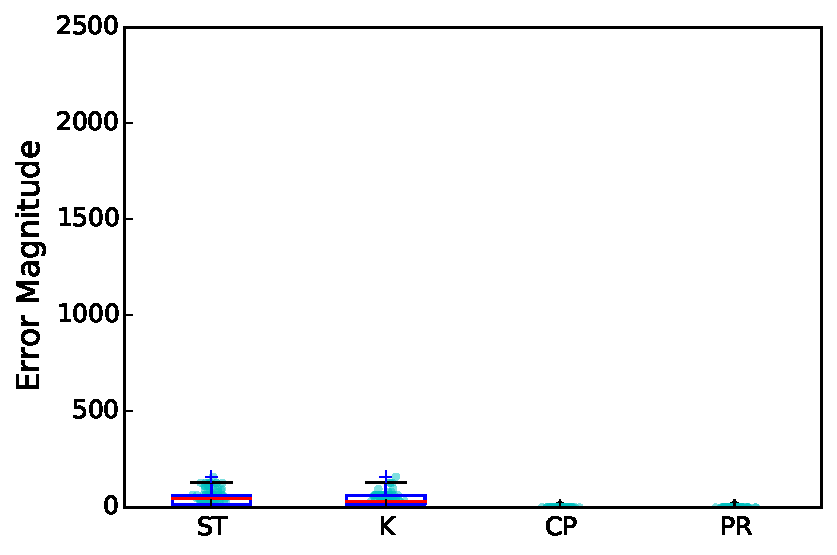
\includegraphics[width=\textwidth,
  height=4cm]{chapter_2_figures/draft_boxplot_balanced_N=8192.pdf} \\ (a)
Balanced, n=8K \\
\end{tabular}
\endminipage 
\minipage[t]{0.30\textwidth}
\begin{tabular}{c}
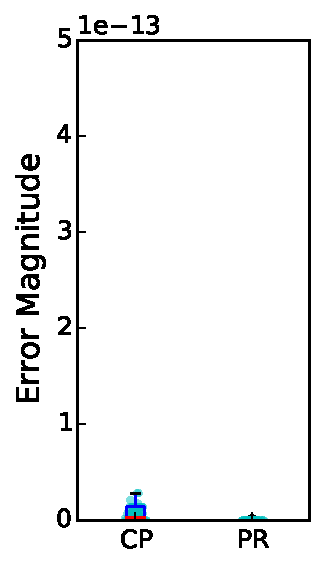
\includegraphics[width=\textwidth,
  height=4cm]{chapter_2_figures/draft_boxplot_balanced_cp_vs_preround_N=8192.pdf}
\\ (b) Zoom into (a) \\
\end{tabular}
\endminipage 
 \\
\minipage[t]{0.40\textwidth}
\begin{tabular}{c}
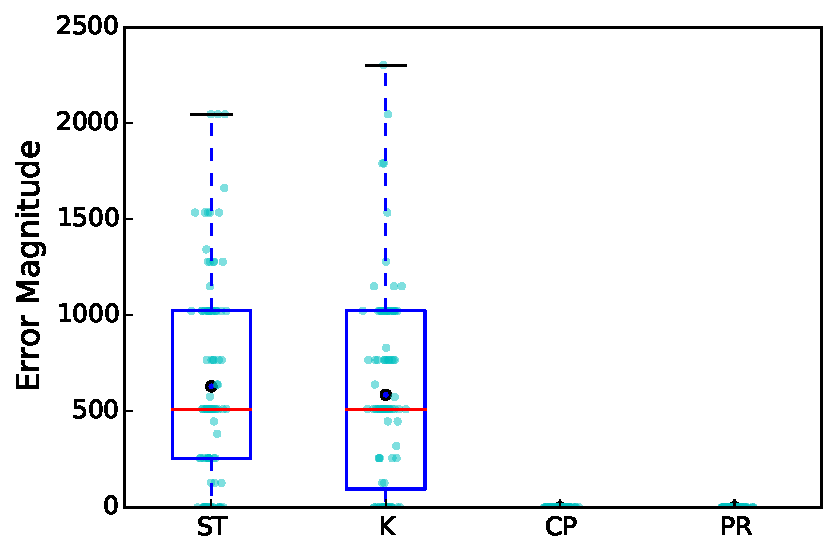
\includegraphics[width=\textwidth, height=4cm]{chapter_2_figures/draft_boxplot_balanced_N=1048576.pdf} \\
(c) Balanced, n=1M\\
\end{tabular}
\endminipage 
\minipage[t]{0.30\textwidth}
\begin{tabular}{c}
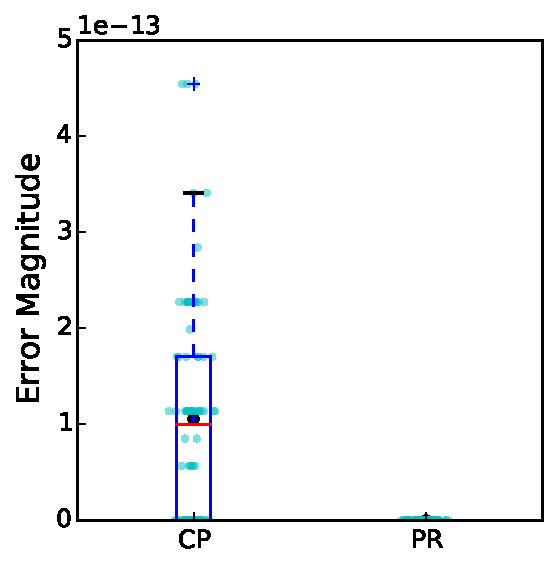
\includegraphics[width=\textwidth, height=4cm]{chapter_2_figures/draft_boxplot_balanced_cp_vs_preround_N=1048576.pdf} \\
(d) Zoom into (c)\\
\end{tabular}
\endminipage 
 \\
\minipage[t]{0.40\textwidth}
\begin{tabular}{c}
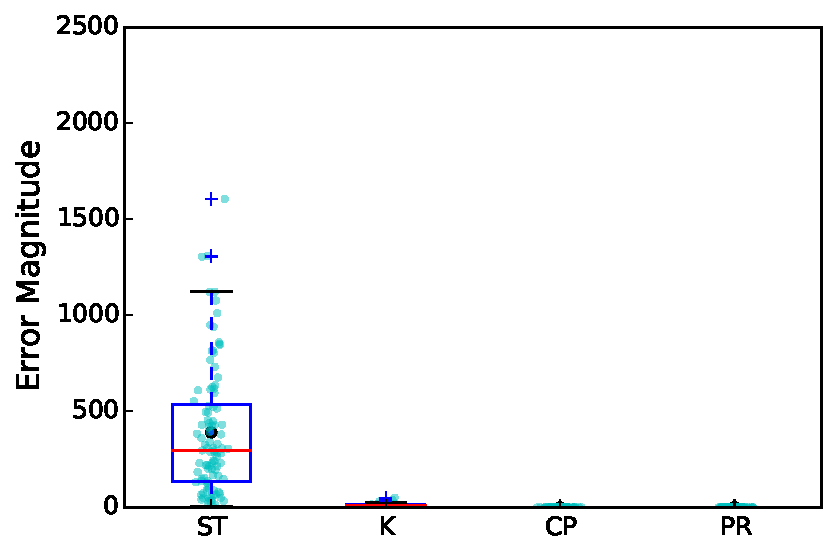
\includegraphics[width=\textwidth, height=4cm]{chapter_2_figures/draft_boxplot_unbalanced_N=8192.pdf} \\
(e) Unbalanced, n=8K \\
\end{tabular}
\endminipage
\minipage[t]{0.30\textwidth}
\begin{tabular}{c}
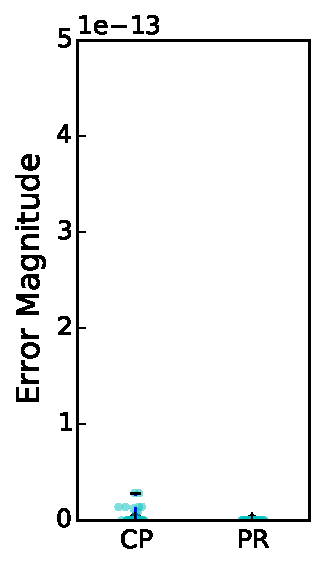
\includegraphics[width=\textwidth, height=4cm]{chapter_2_figures/draft_boxplot_unbalanced_cp_vs_preround_N=8192.pdf} \\
(f) Zoom into (e)\\
\end{tabular}
\endminipage 
 \\
\minipage[t]{0.40\textwidth}
\begin{tabular}{c}
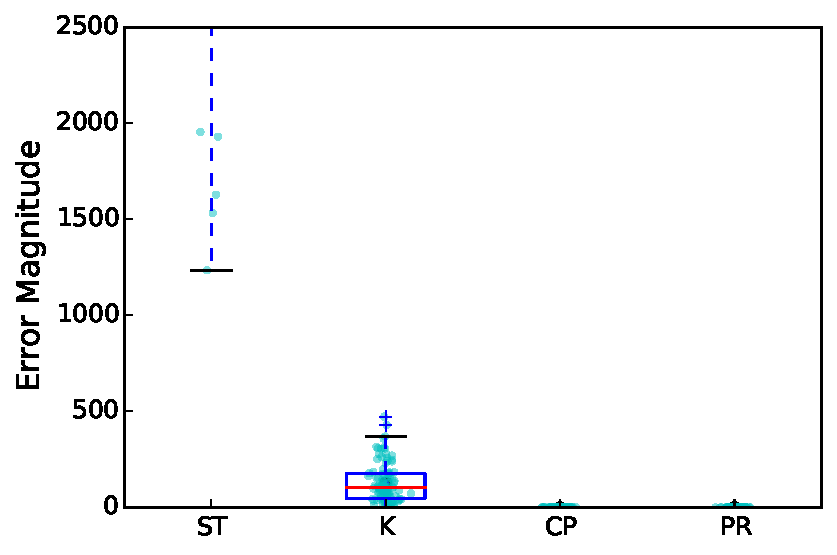
\includegraphics[width=\textwidth, height=4cm]{chapter_2_figures/draft_boxplot_unbalanced_N=1048576.pdf} \\
(g) Unbalanced, n=1M\\
\end{tabular}
\endminipage 
\minipage[t]{0.30\textwidth}
\begin{tabular}{c}
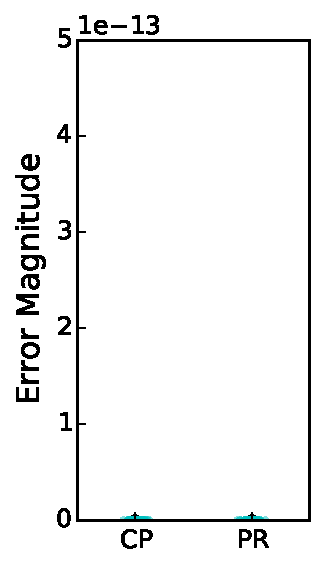
\includegraphics[width=\textwidth, height=4cm]{chapter_2_figures/draft_boxplot_unbalanced_cp_vs_preround_N=1048576.pdf} \\
(h) Zoom into (g)\\
\end{tabular}
\endminipage 
  \caption{Error distributions for the four summation algorithms
    considered in this chapter for balanced and unbalanced reductions:
    three at a smaller (8K leaves) and one at higher (1M leaves)
    levels of concurrency.}
\label{fig:boxplot}
\end{figure*}

The effect of nondeterminism in the reduction tree is exhibited in
Figures~\ref{fig:boxplot}. For a given summation algorithm, the
distribution of data points and width of the box indicate how much the
sum tends to vary when the overall shape of the reduction tree is
constant but the arrangement of summands to its leaves is
variable. Within the subfigures, we see that although Kahan summation
tends in general to produce more reproducible sums than standard
summation, only composite precision and prerounded summations offer
reproducible numerical accuracy at an acceptable level.  Across a row
of subfigures, we see that as the level of concurrency rises, the
absolute error in the sum rises as expected. However, by comparing
results across a column of subfigures, for example, the ST data from
Figure~\ref{fig:boxplot}(a) and the ST data from
Figure~\ref{fig:boxplot}(e), we see that much more variation in the
sum occurs when the tree is unbalanced than when it is balanced for
the standard summation algorithm. To cope with intermittent faults and
inconsistently available resources, we expect that the reduction trees
employed by an exascale system will vary not only in terms of
arrangement of data among their leaves but also in overall shape. We
conclude that because of the difference in reproducibility observed
for differently shaped reduction trees, exascale applications will
need to maintain awareness of the degree of fluctuation in reduction
tree shape and employ more robust reduction operators accordingly.

\subsection{Effect of Concurrency, Conditioning, and Dynamic Range}

For a fixed level of concurrency, the mathematical properties of the
summands can have a significant impact on the sensitivity of the sum
to variations in the reduction tree. In the previous section, we
considered a set of values with a fixed condition number $k$ and
dynamic range $dr$.  In this section, we examine the effects of
varying $k$ and $dr$ at a fixed level of concurrency $n=1M$; varying
$dr$ and $n$ at a fixed $k$; and varying $k$ and $n$ at a fixed
$dr$. We represent the spaces of $(k, dr)$, $(n, dr)$, and $(n, k)$ as
a grid of cells, where for each cell we generate a set of
floating-point values with the cell parameters. The degree to which
these sets of values can be summed reproducibly is tested. For all
sets of summands under consideration, we measure their potential for
irreproducibility by computing their sum with 1,000 distinct, balanced
reduction trees obtained by permuting the assignment of summands to
leaves. As in the our previous experiment we test four summation
algorithms. However, we display results only for the first three
because the composite precision and prerounded summations performed
identically for all sets of inputs considered. Once all the sums have
been computed for a cell, the error in each sum is calculated with
respect to an accurate reference sum, which we compute in quad-double
precision using the GNU MPFR high-precision library. To visualize the
level of irreproducibility observed, we compute the standard deviation
of the errors and shade the cell according to that
value. Figure~\ref{fig:cellsreductions} illustrates the process in a
visual (and more intuitive) way.
\begin{figure}[!htb]
  \centering
  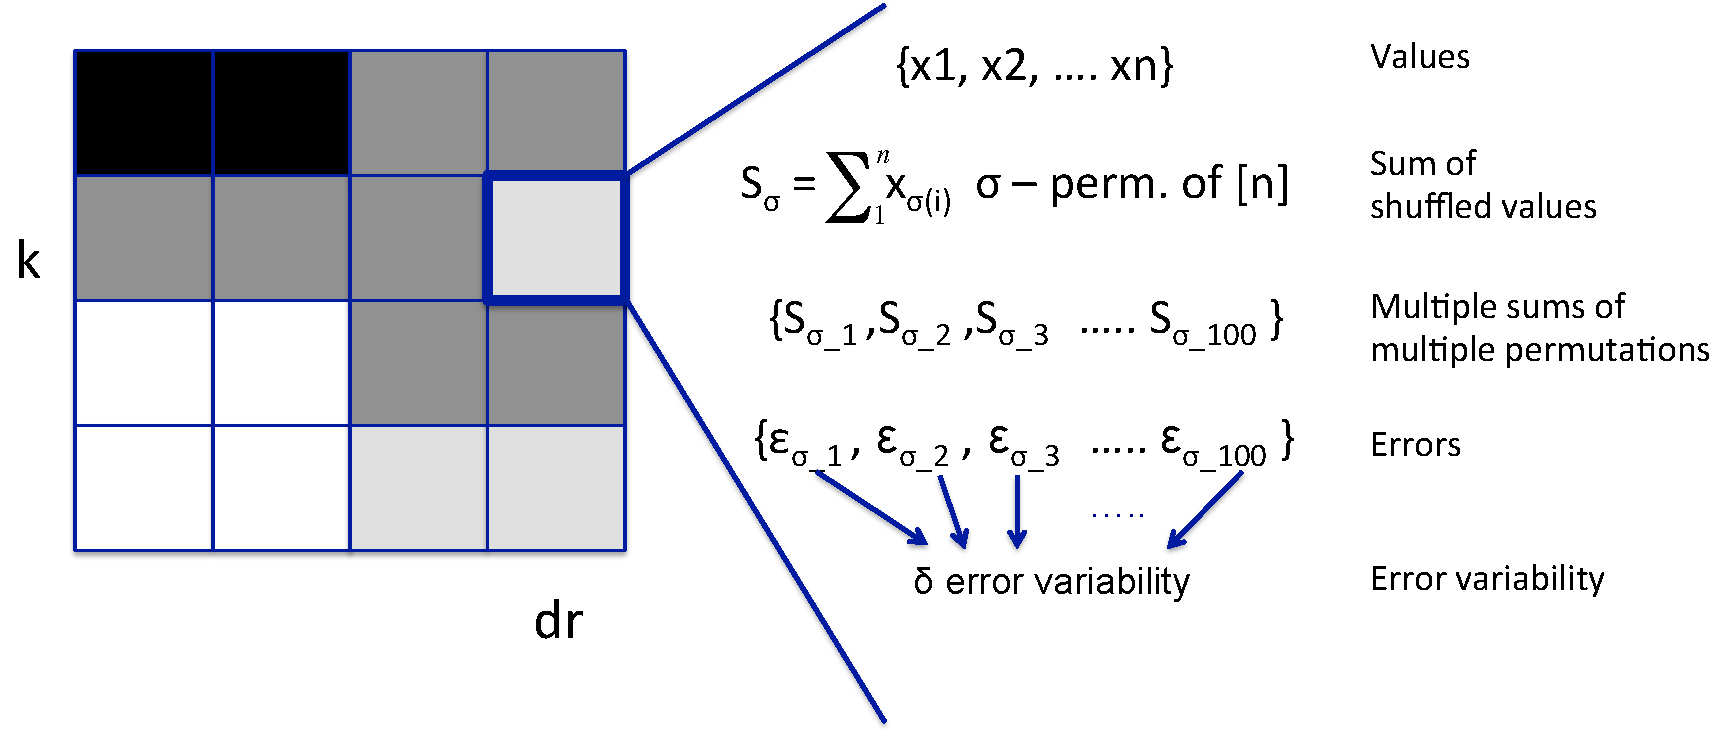
\includegraphics[width=0.8\textwidth]{chapter_2_figures/cell.pdf}
  \caption{Overview of the grid with its cells used to study the
    effect of concurrency, conditioning, and dynamic range.}
  \label{fig:cellsreductions}
\end{figure}

Figure~\ref{fig:k_vs_dr} shows how position in the space of possible
$(k, dr)$ values influences the variability of a sum at a fixed level
of concurrency. The darker cells toward the top and right of the two
leftmost grids indicate sets of summands whose sums varied much more
than the level of variation observed for sets of summands with lower
condition number. The darkest cell in the standard summation grid is
anomalous but likely due to particularly severe subtractive
cancellation, since its condition number is large. The rightmost grid
shows that for all considered sets of summands, the result according
to the composite precision summation did not vary with changes in the
reduction tree.
\begin{figure*}[!htb]
\centering
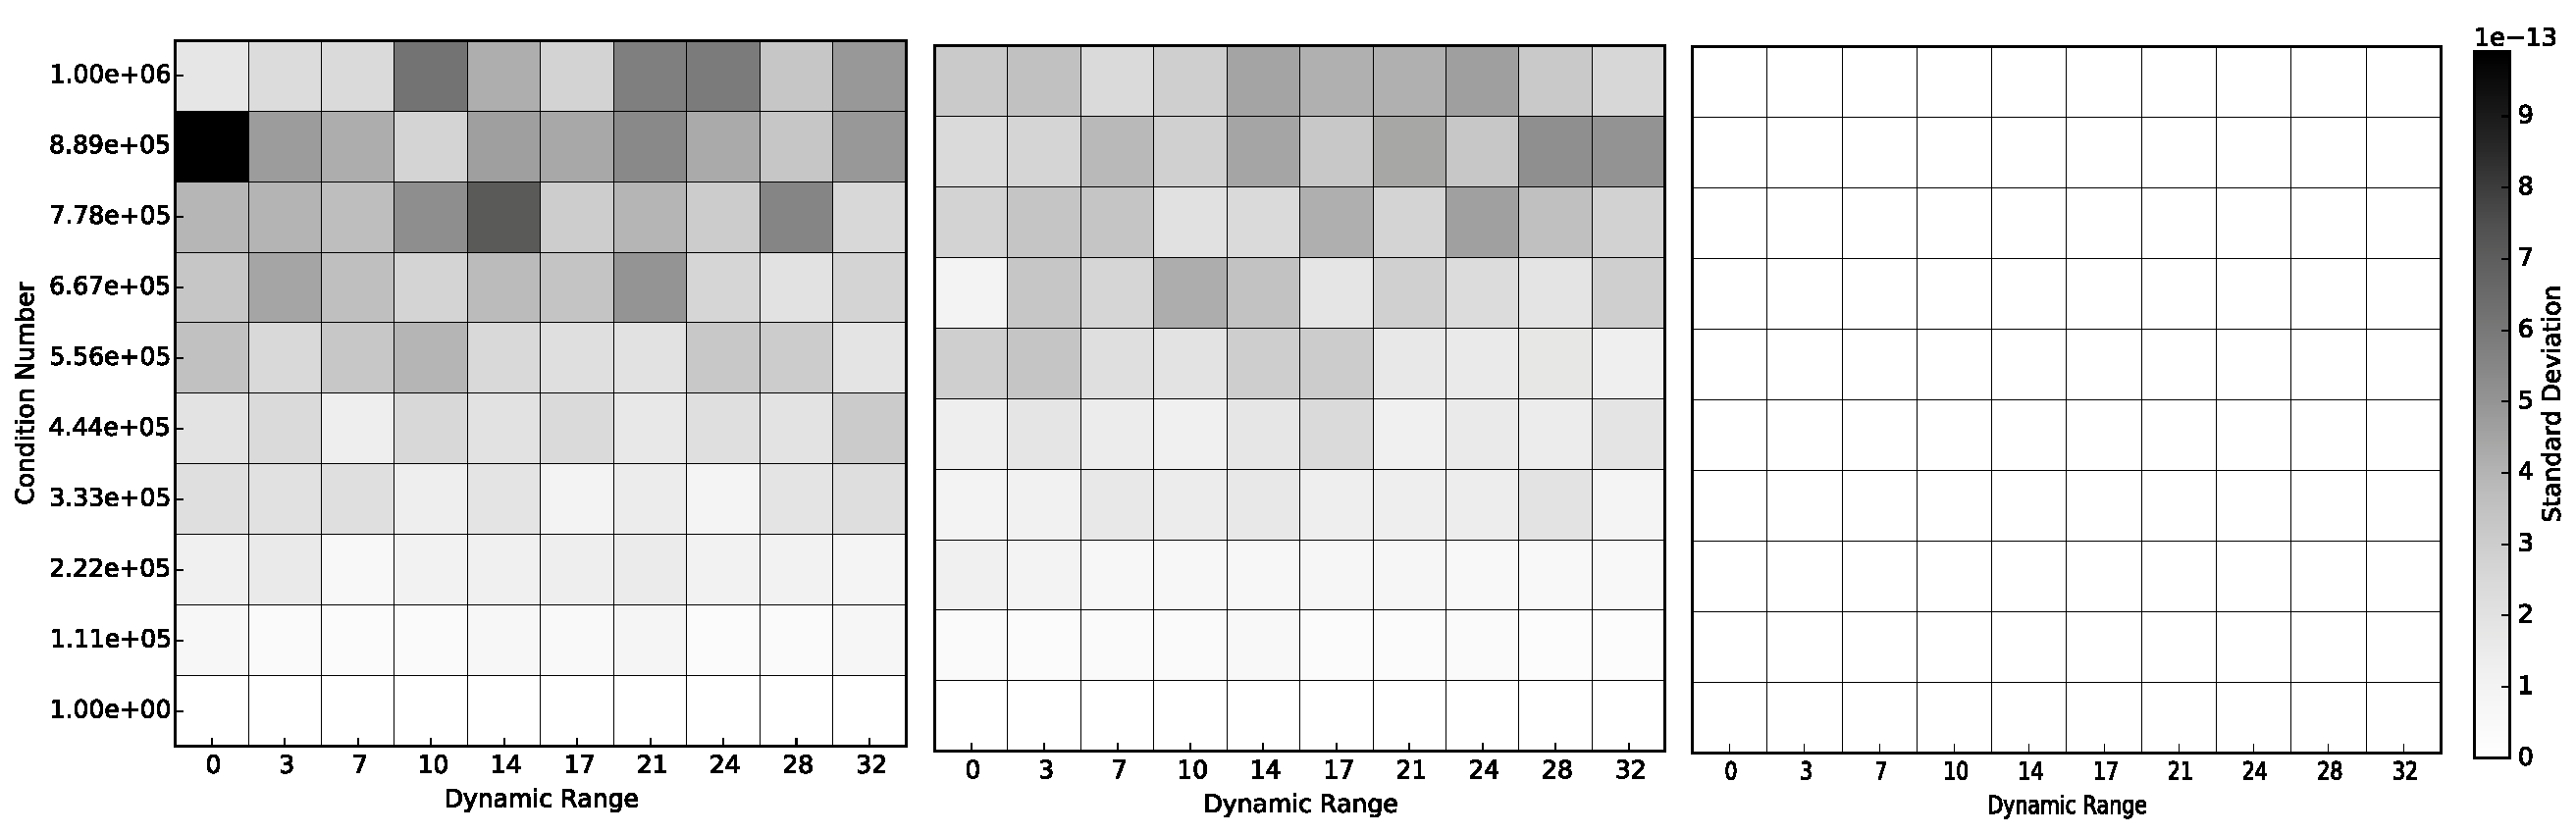
\includegraphics[width=\textwidth]{chapter_2_figures/fig_kvsDr.pdf} \\
\caption{Standard deviation errors for standard summation (left),
  Kahan summation (middle), and composite precision summation (right)
  for different $(k, dr)$ values and fixed concurrency $n$.}
\label{fig:k_vs_dr}
\end{figure*}

Figure~\ref{fig:n_vs_dr} presents the impact of dynamic range for a
fixed condition number. For these grids, each cell's summands have
condition number $k=1$ so that the ability of dynamic range to
estimate alignment error can be assessed. Note that the
scale by which the cells are shaded for these grids is not the same as
for the grids examining the $(k, dr)$ or $(n, k)$ spaces. There is a
tendency for high-concurrency, high-dynamic-range cells to exhibit
greater variability; but the most valuable lesson from these
visualizations is that dynamic range exerts much less influence over
variability of the sums than does the condition number, as seen in
Figure~\ref{fig:n_vs_k}. Here, we observe a strong relationship
between high variability of sums and sets of summands with high
condition number. These results suggest the need for
applications to maintain awareness of the mathematical properties of
sets of floating-point values generated at runtime, and if the
reduction tree is expected to change from run to run, to select
reduction algorithms that take those mathematical properties into
account.
\begin{figure*}[!htb]
\centering
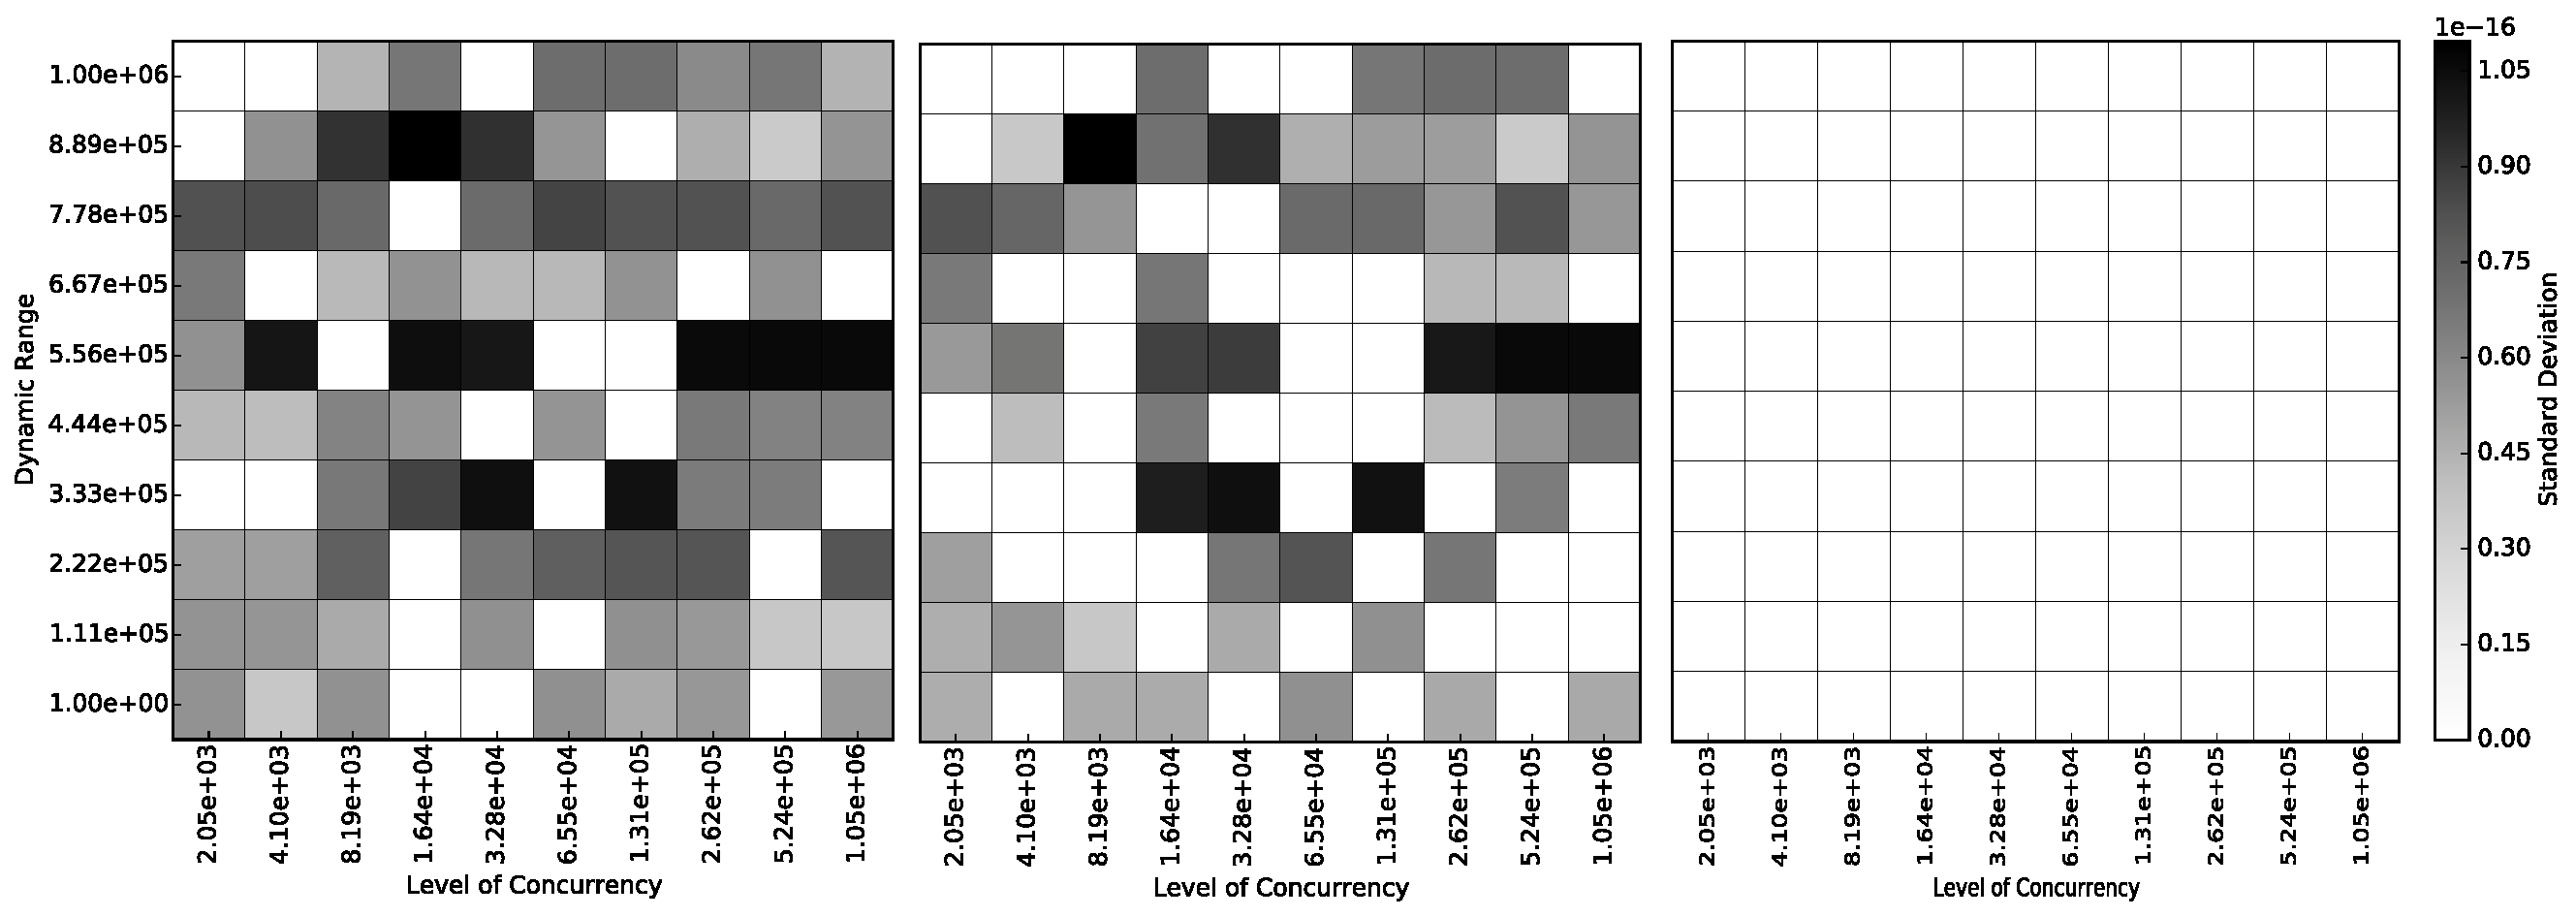
\includegraphics[width=\textwidth]{chapter_2_figures/fig_NvsDr.pdf} \\
\caption{Standard deviation errors for standard summation (left),
  Kahan summation (middle), and composite precision summation (right)
  for different $(n, dr)$ values and fixed condition number $k$.}
\label{fig:n_vs_dr}
\end{figure*}
\begin{figure*}[!htb]
\centering
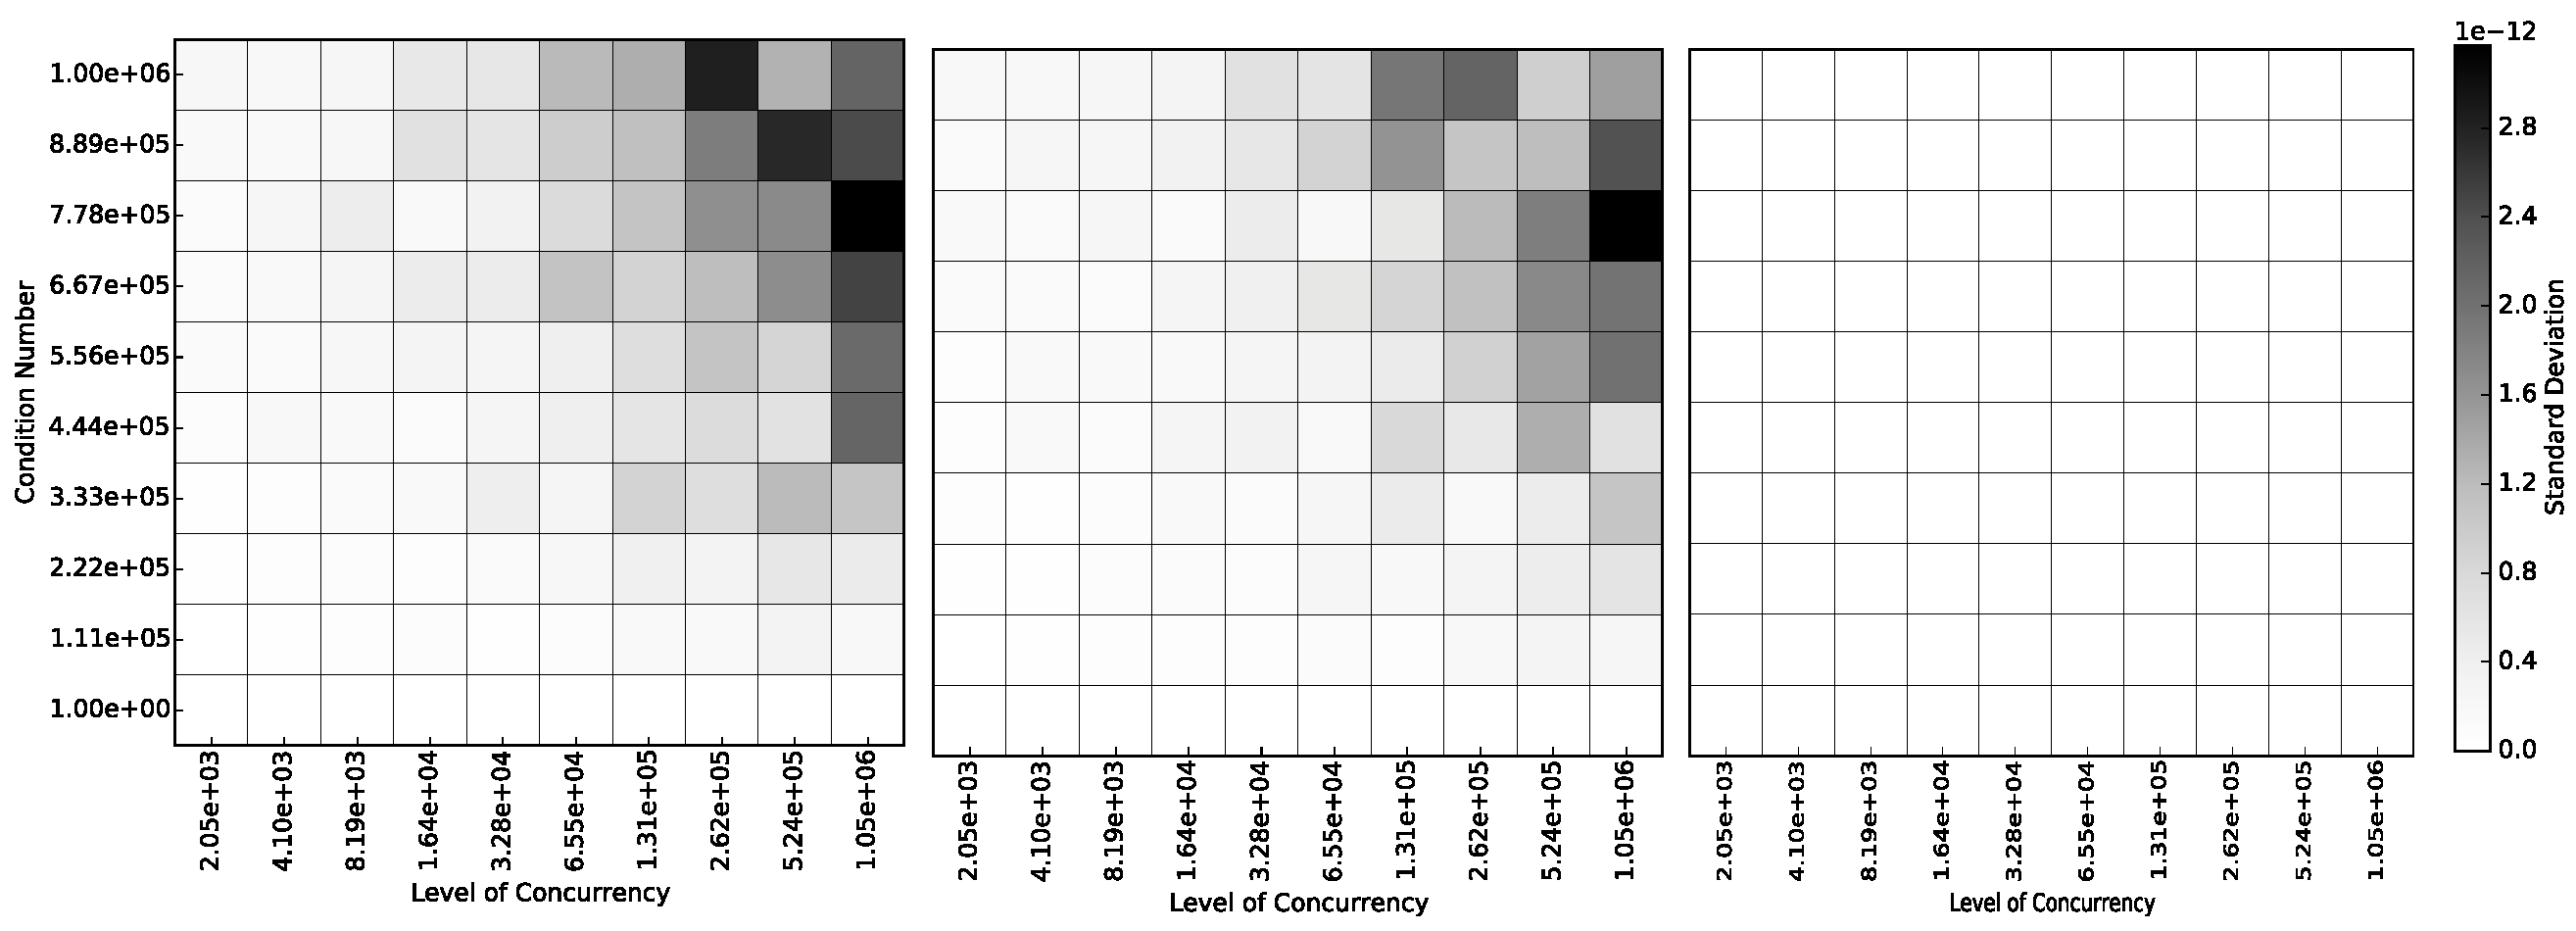
\includegraphics[width=\textwidth]{chapter_2_figures/fig_Nvsk.pdf} \\
\caption{Standard deviation errors for standard summation (left),
  Kahan summation (middle), and composite precision summation (right)
  for different $(n, k)$ values and fixed dynamic range $dr$.}
\label{fig:n_vs_k}
\end{figure*}

\subsection{Intelligent Selection of Reduction Algorithms} 

Techniques such as compensated summation can reduce the amount of
variability observed in repeated summation when the summation order
changes from run to run. However, application developers are faced
with the challenge of selecting the summation algorithm that gives
them the level of reproducibility and accuracy required by their
application. At exascale, judicious selection of reduction algorithms
will be vital so that application-specific reproducible numerical
accuracy can be achieved at tolerable cost. In contrast to the old
notion of bitwise reproducibility, application-specific
reproducibility requires developers to specify an upper bound on the
amount of variability in the values of floating-point reductions that
can be tolerated while maintaining the trustworthiness of the
application's output.

A set of floating-point values occupies a position in a complex
parameter space: the number of values, reduction tree, condition
number, and dynamic range all exert influence over which reduction
algorithm can cost-effectively achieve a specified level of
reproducibility. Our data suggests that in order to avoid exceeding a
fixed level of variability, if one cannot control the reduction tree,
it may be possible to use standard summation when values are uniform
and well-conditioned and to adaptively switch to a more robust
summation algorithm if the values to be reduced become less uniform or
less well-conditioned. We argue that unlike attempting to achieve
reproducible numerical accuracy by additional data movement, as would
be required to fix a reduction tree, estimable quantities such as
condition number and dynamic range can guide runtime selection of a
reduction operator with the appropriate performance/reproducibility
tradeoff for the application at hand. In Figure~\ref{fig:spec}, we
show the $(k, dr)$ grid for several error variability thresholds. Here
cells are shaded based on the cheapest summation algorithm that
achieves a given degree of reproducibility at that cell. As we reduce
the variability threshold, effectively stepping toward bitwise
reproducibility with smaller and smaller thresholds, we see that
increasingly costly summation algorithms are required for the more
challenging regions in the space (i.e., those with high condition
number and high dynamic range).
\begin{figure*}[!htb]
  \centering
  \minipage[t]{\textwidth}
  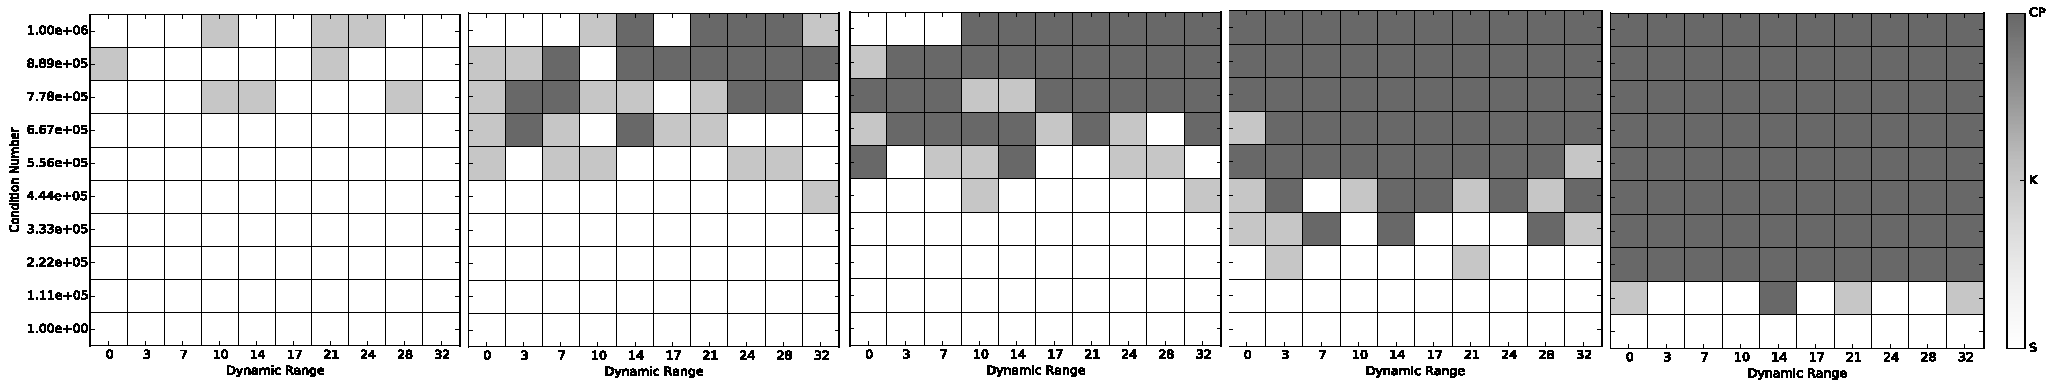
\includegraphics[width=\textwidth]{chapter_2_figures/spectrum.pdf}
  \caption{Selection of the cheapest but acceptably accurate reduction
    algorithm among the Kahan (K), composite precision (CP), and
    prerounding (PR) algorithms for different error variability
    thresholds (left to right: $t=5e-13, 3e-13, 2.5e-13, 1.5e-13,
    5e-14$).}
  \label{fig:spec}
  \endminipage
\end{figure*}

Achieving reproducible numerical accuracy by intelligent runtime
selection of reduction algorithms depends on being able to assess the
mathematical properties of the floating-point values to be reduced. We
show that if this assessment can be done, one can avoid using a more
expensive reduction algorithm when a cheaper one will do. These
results present a strong case for further research into tools that, at
exascale, profile parameters of interest (e.g., $n$, $k$, $dr$, and
tree shape) at runtime and apply cheaper but acceptably accurate
reduction algorithms to subtrees based on the profile.

\section{Lessons Learned}
\label{sec:conclusion}
In this chapter we tackle the first of our two challenges (i.e., the
numerical challenge). We identify relevant parameters that, when
analyzed in concert, can provide insight into intelligent selection of
reduction algorithms to achieve reproducible numerical accuracy on
soon-to-exist exascale platforms.

Three main observations emerge from our study on reproducible
numerical accuracy. First, reduction tree shape has a large impact on
reproducible numerical accuracy.  Second, mathematical properties of a
set of summands have an impact on the reproducibility of their sum. In
applications where the conditioning and dynamic range can change
dramatically over the course of the runtime, this effect is especially
relevant.  Third, we show that if we fix a target level of
reproducibility, we can classify regions of the parameter space by the
cheapest algorithm that achieves the desired level of reproducibility
at that point in the space. This is an important step toward
implementing intelligent runtime selection of reduction operators on
future exascale platforms.
    % This file (chap2.tex) contains the text
                   % for Chapter 2.

\chapter{The Debugging Challenge} \label{chap3}

\section{Introduction}

In this chapter we first provide an overview of the record-and-replay
approach for debugging a class of non-deterministic applications and
describe the properties of existing record-and-replay tools. We then
present our extension to the record-and-replay approach together with
the performance of the integration of our extension into a
production-grade record-and-replay tool.

\section{Record-and-Replay Approach and Tools} 

To overcome the impediments to debugging associated with
non-deterministic executions, a class of debugging aids collectively
referred to as record-and-replay tools have been developed. These
tools allow developers to record one execution of a target
application, then replay it exactly. In general, record-and-replay
tools must establish an order of events during the recorded execution,
then write a representation of that order to some form of persistent
storage. The exact data that must be recorded depend on what
assumptions can be made about the form of nondeterminism the target
application exhibits. Figure~\ref{fig:rrframework} shows a general
overview of these tools' framework.
\begin{figure}[!ht]
    \centering
    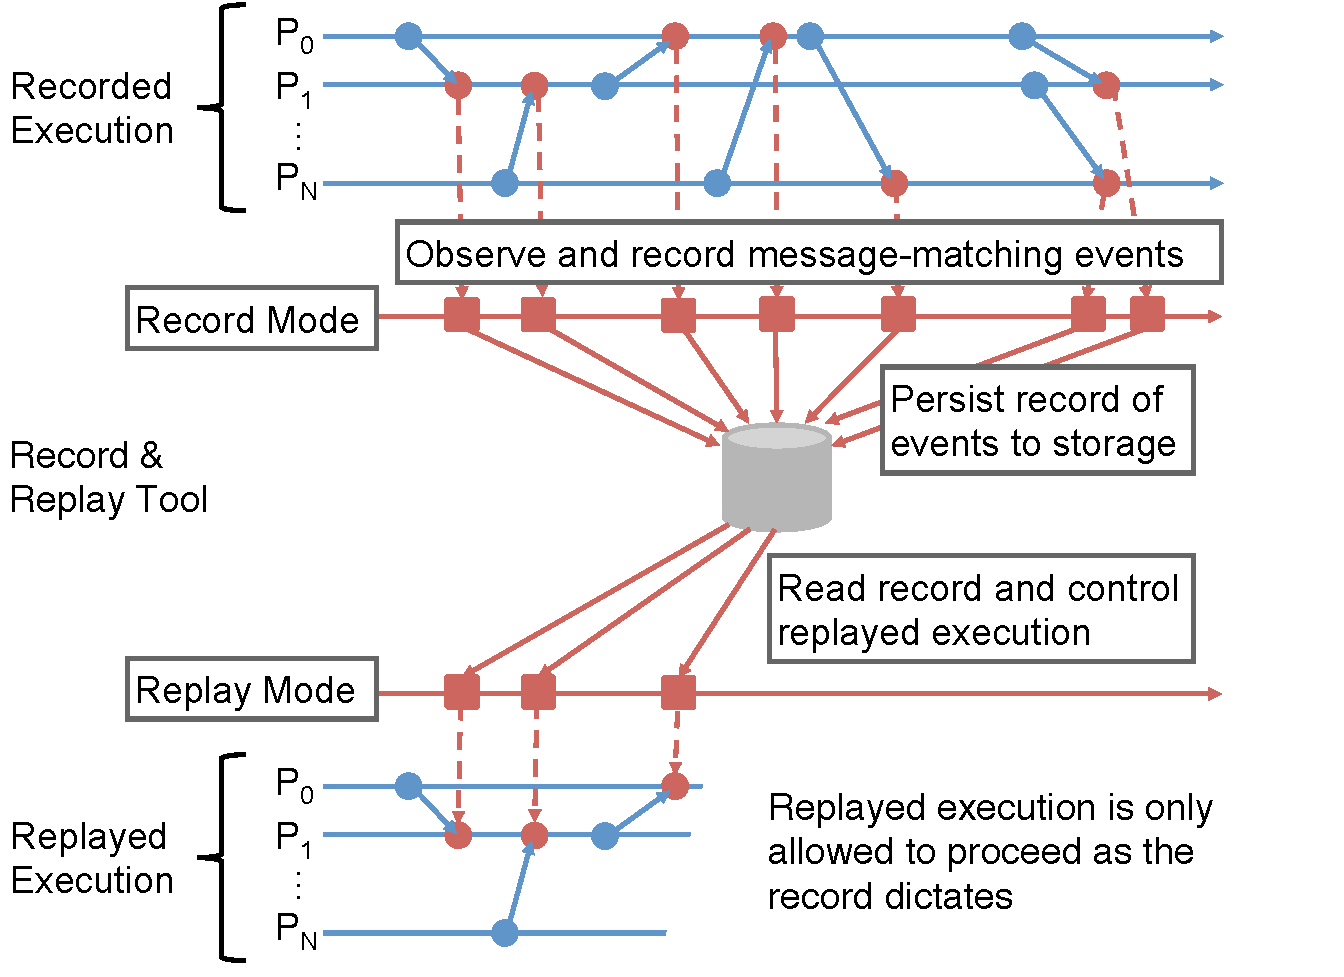
\includegraphics[width=0.8\linewidth]{chapter_3_figures/rrframework.pdf}
    \caption{General overview of a record-and-replay framework.}
    \label{fig:rrframework}
\end{figure}

Necessary behaviors of record-and-replay tools can be sorted in two
groups: during recording and during replay. During recording, a tool
must observe communication events in an application's execution and
store (or write) information that unambiguously orders the observed
events into a record. One way to do this task is with logical clocks
and metadata (described in the next section). Metadata in message
passing applications include processes' rank, tag, and communication
event type (e.g., completion of a receive vs. invocation of
Test-family function).

During replay, a tool must read (or query) the record followed by
buffering and re-ordering communication events in the subsequent
execution. Correctness of the replay depends on assumptions about the 
application (e.g., is the application send-deterministic)~\cite{CommunicationDeterminism:Cappello:2010}
and inductive arguments (e.g., the $n^{th}$ event is replayed correctly as a
consequence of the $n-1^{th}$ event being replayed correctly).

Existing record-and-replay tools fall into two broad categories:
data-replay and order-replay. These categories refer to the content
that is traced by the tool during recording.  Specifically,
data-replay tools record the total content of messages, whereas
order-replay tools opt instead to record the messages' relative
ordering. The state of the art in record-and-replay takes the
order-replay approach primarily due to the significant reduction in
record size it provides by not recording possibly large message
payloads in addition to the necessary message order data.

The earliest record-and-replay tools employed the data-replay
approach, but attempt to mitigate the growth of record size via
selectively recording only those messages deemed at runtime to be a
source of non-determinism.  Netzer and Miller employ vector clocks to
identify racing messages and thus restrict the number of necessarily
recorded messages in their tool~\cite{OptimalTracing:Netzer:1992}.
Later work by Cl\'emec\c on \textit{et al.} used a similar vector
clock approach, but extended the tool's capabilities to record
non-blocking probes as well as wildcard
receives~\cite{RaceDetection:Clemencon:1995}. Despite these
techniques' applicability at the time of their creation, their use of
vector clocks makes them prohibitively expensive for modern HPC
systems, since each message is saddled with a vector of $n$ elements
where $n$ is the number of processors in the
system~\cite{VectorClocksI:Fidge:1988}.

Later record-and-replay tools embraced the order-replay design,
recognizing that despite the need to make stronger assumptions about
message contents than data replay tools do, increasingly large systems
necessitate the smaller record sizes that order-replay tools can
deliver.  One early tool in this domain was the Nondeterministic
Program Evaluator (NOPE) developed by Kranzlm\"uller and
Volkert~\cite{NOPE:Kranzlmuller:1999}. Last, Clock-Delta Compression
(CDC)~\cite{ClockDeltaCompression:Sato:2015} is the state-of-the-art
approach to record-and-replay that aims to overcome the problem of
large record size that renders traditional record-and-replay
techniques inapplicable at extreme scale. We build our work on top of
this approach that we describe in the next section.

\section{Clock-Delta Compression}

Clock-Delta Compression (CDC) establishes an order on communication
events during recording by piggybacking logical clocks on messages
between processes, and applies a novel compression pipeline to the
record that leverages properties of the piggybacked clocks. In this
section, we provide an overview of the CDC record format, a high-level
description of the compression pipeline, and describe the role of the
piggybacked logical clocks with respect to the record format and the
compression pipeline.

The CDC record format is a data structure built up during recording
that contains sufficient information about interprocess communication
events to enable deterministic replay of the recorded execution. The
record format consists of three main parts: the
\textit{with-next-table}, the \textit{unmatched-test-table} and the
\textit{matched-test-table}. The \textit{with-next-table} records when
multiple incoming messages match with a single receive request, as can
occur if MPI\_Testsome, MPI\_Testall, MPI\_Waitsome, or MPI\_Waitall
are employed by the application.  The \textit{unmatched-test-table}
records instances of MPI\_Test-family functions being called on a
receive request when no matching send exists, as can occur when a
polling loop of test calls is used to complete a non-blocking
receive. Finally, the \textit{matched-test-table} records the actual
matches between receive requests and incoming messages. This component
of the record format is our focus since the most dramatic reductions
in record size that CDC offers apply to the
\textit{matched-test-table}. Moreover, the specific implementation of
the underlying logical clock protocol directly effects the
compressibility of the \textit{matched-test-table}.

The CDC compression pipeline is applied to the CDC record format
during recording and consists of three stages: permutation encoding,
linear-predictive encoding (LPE), and lossless compression. The
permutation encoding stage is applied only to the
\textit{matched-test-table}, whereas LPE is applied to components of
the \textit{matched-test-table} and \textit{unmatched-test-table}. The
lossless compression stage is applied to the entire record after
permutation encoding and LPE. We provide the description of the
algorithm for permutation encoding in
Section~\ref{sec:permutation_encoding} due to the critical reduction
in size of the \textit{matched-test-table} that it provides and the
degree to which its functionality is intertwined with the notion of a
logical clock ticking policy described in Section
~\ref{sec:logical_clocks}.

\section{Logical Clocks} \label{sec:logical_clocks}

Logical clocks, originally defined by Lamport
in~\cite{LogicalClocks:Lamport:1978}, provide a method for
establishing a partial order on events in a distributed system. Within
the context of the CDC record-and-replay technique, we describe 
the rules of the logical clock protocol that CDC employs, we define
the notion of logical clock ticking policy, and we discuss how
recording events are distinguished by the logical clock values
associated to them.

CDC establishes a partial order on all communication events that occur
during recording by maintaining in each process $p$ an integer value
referred to as the local clock of that process.  Whenever $p$ sends a
message to another process, $p$ attaches a copy of its local clock to
the message, then increments its local clock by some value $t$,
hereafter referred to as a ``tick''.  When another process $q$ receives
$p$'s message, it sets its own local clock to the maximum of its
current value and the value attached to the message it just
received. Then $q$ increments its local clock by some amount (i.e.,
$q$ ticks its local clock). Two immediate consequences of this
protocol are that within a process, if an event $e_0$ occurred before
another event $e_1$, the logical clock values associated to those
events (e.g., $c_0$ and $c_1$) satisfy $c_0 < c_1$, and between a
sender process and a receiver process, a send event's clock will
always be less than its corresponding receive event's clock.

So far we have discussed logical clocks' ticks without specifying what
values they must take. In Lamport's paper on logical
clocks~\cite{LogicalClocks:Lamport:1978}, ticks are assumed to always
equal $1$, but in fact all that is necessary to establish a partial
order is that the ticks have positive value. In the context of
record-and-replay, since the replayed execution must exactly match the
recorded execution, we require the additional constraint that the
ticks be deterministic (i.e., during replay), for all processes, the
$i$th tick applied to a process's local clock must match the $i$th
tick that was applied to its local clock during recording. We define a
\textit{logical clock ticking policy} to be a mechanism for deciding
what value each tick applied to each process's logical clock will
take.

\section{In- and Out-of-order Received Messages}

In this section, we define the concept of an event (e.g., message
receive) being in-order or out-of-order with respect a logical clock
reference order, and how out-of-order messages impact the size of the
\textit{matched-test-table}. In CDC, every receive completion event is
associated to a logical clock value that is piggybacked on a received
message. Specifically, each process has a ``local clock'' (LC) that is
initially zero. When a process (e.g., $P_0$) sends a message, its LC
is attached to the message as the ``sent clock'' (SC). Afterward, the
sending process's LC is incremented by one. When a process (e.g.,
$P_1$) receives a message from another process (e.g., $P_0$), it
updates its LC by the Lamport Clock protocol $LC = max(LC, SC) + 1$
and records the receive event. The list of SC values that every
receiving process builds up over the course of recording an execution
defines whether a received message is in-order or out-of order: if the
new SC is larger than the previous received SC, then the message is
in-order; if it is smaller, then then the message is
out-of-order. The SC values are the input to the permutation
encoding step of the CDC compression pipeline, and the degree of
monotonicity in this list of values determines the effectiveness of
the compression. Moreover, the list of SC values is not the same
logical clock value that any receiving process updates its local clock
to, and as such does not impose a partial order on events in the same
way. Figure~\ref{fig:inandout} shows examples of in-order or
out-of-order messages: Figure~\ref{fig:inandout}.(a) shows an example
of an in-order received message and Figure~\ref{fig:inandout}.(b) shows
an example of an out-of-order received message. In
Figure~\ref{fig:inandout}.(a), the SC of $P_0$ is 17; because the SC
value is larger than the precious SC of $P_1$ (in the figure the
$SC_{previous}$ is 15), the received in-order message is annotated in
the SC list but will not be recorded in the \textit{matched-test
  table}. This is not the case in Figure~\ref{fig:inandout}.(b) in
which the the SC of the sending $P_0$ is still 17 but the previously
annotated SC is larger (i.e., equal to 19), causing the recording of
the event in the \textit{matched-test table}.
\begin{figure}[!htb]
\centering
\minipage[t]{0.45\textwidth}
\begin{tabular}{c}
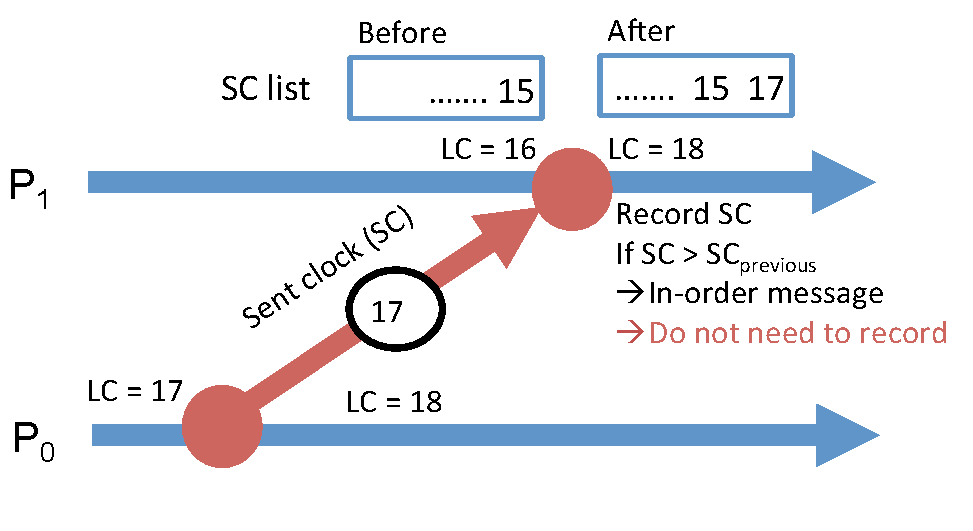
\includegraphics[width=\textwidth,
  height=6cm]{chapter_3_figures/inorder.pdf} \\ (a) In-order \\
\end{tabular}
\endminipage
\minipage[t]{0.45\textwidth}
\begin{tabular}{c}
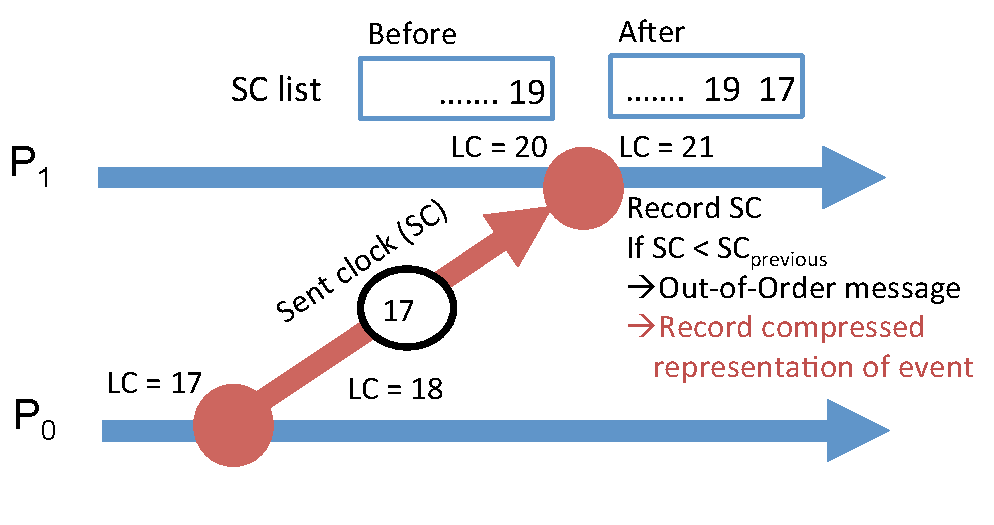
\includegraphics[width=\textwidth,
  height=6cm]{chapter_3_figures/outoforder.pdf} \\ (b) Out-of-order\\
\end{tabular}
\endminipage
\caption{Example of in-order (a) and out-of-order (b) messages.}
\label{fig:inandout}
\end{figure}

Figure~\ref{fig:exampleinandout} show a larger five-stage example in
which multiple messages are received by a process $P_0$. For each
stage, the upper figure shows the snapshot with the sent and received
messages up to that point for process $P_0$; the bottom figure shows
the associated SC list. In Stage 1, $P_0$ receives a message from, for
example, $P_1$. $P_0$ updates its local clock (LC), which was
initially equal to 1, by using the Lamport Clock protocol to 4 (i.e.,
LC of $P_0$ becomes the max of LC and SC plus one) and temporally
records the time of the received message (i.e., SC time is equal to
3). In Stage 2, $P_0$ receives a second message from $P_2$; $P_0$
updates its LC following the same procedure as in Stage 1. The LC of
$P_0$ becomes 6 and the process also records the received SC value (in
this case SC is equal to 5). We observe that at the end of Stage 2 the
received clocks' values are monotonically increasing ``in-order''. The
process takes note of the message's SC but does not forward the SC
value to its \textit{matched-test table}. In Stage 3, $P_0$ sends
messages. Its LC increases each time a send is initiated but no
clock is recorded. In Stage 5, two additional messages from a
different process than $P_1$ are received by $P_0$. This time the
first message is out-of-order (i.e., with a SC equal to 4 smaller than
5) and is thus used for building the process'~\textit{matched-test
  table}. The second is in-order (i.e., with a SC equal to 7 larger
than 4) and is not considered for the process'~\textit{matched-test
  table}.
\begin{figure} [!htb]
    \centering
    \begin{minipage}{0.20\textwidth}
        \includegraphics[width=0.9\linewidth]{chapter_3_figures/record_step_2}
        \label{fig:record_step_2}
    \end{minipage}%
    \begin{minipage}{0.20\textwidth}
        \includegraphics[width=0.9\linewidth]{chapter_3_figures/record_step_3}
        \label{fig:record_step_3}
    \end{minipage}% 
   \begin{minipage}{0.20\textwidth}
        \includegraphics[width=0.9\linewidth]{chapter_3_figures/record_step_4}
        \label{fig:record_step_4}
    \end{minipage}%
    \begin{minipage}{0.20\textwidth}
        \includegraphics[width=0.9\linewidth]{chapter_3_figures/record_step_5}
        \label{fig:record_step_5}
    \end{minipage}%
    \begin{minipage}{0.20\textwidth}
        \includegraphics[width=0.9\linewidth]{chapter_3_figures/record_step_6}
        \label{fig:record_step_6}
    \end{minipage}%
\\
    \begin{minipage}{0.20\textwidth}
        \stackunder[5pt]{\includegraphics[width=\linewidth]{chapter_3_figures/received_clocks_2}}{Stage 1}
        \label{fig:received_clocks_2}
    \end{minipage}%
    \begin{minipage}{0.20\textwidth}
        \stackunder[5pt]{\includegraphics[width=\linewidth]{chapter_3_figures/received_clocks_3}}{Stage 2}
        \label{fig:received_clocks_3}
    \end{minipage}%
    \begin{minipage}{0.20\textwidth}
        \stackunder[5pt]{\includegraphics[width=\linewidth]{chapter_3_figures/received_clocks_4}}{Stage 3}
        \label{fig:received_clocks_4}
    \end{minipage}%
    \begin{minipage}{0.20\textwidth}
        \stackunder[5pt]{\includegraphics[width=\linewidth]{chapter_3_figures/received_clocks_5}}{Stage 4}
        \label{fig:received_clocks_5}
    \end{minipage}%
    \begin{minipage}{0.20\textwidth}
        \stackunder[5pt]{\includegraphics[width=\linewidth]{chapter_3_figures/received_clocks_6}}{Stage 5}
        \label{fig:received_clocks_6}
    \end{minipage}%
    \caption{Example of a five-stage execution in which in-order and out-of-order
      messages are received by process $P_0$. We show in-order receives in stages 
      1, 2, 3, and 5. We show an out-of-order receive in stage 4, in which a sent
      clock of 4 is received after $P_0$ has already received a larger sent clock
      of 5.}
    \label{fig:exampleinandout}
\end{figure}

\section{Permutation Encoding} 
\label{sec:permutation_encoding}

During recording, the process receiving messages with the attached
logical clock values builds up the \textit{matched-test table}. The
table collects only information on out-of-order messages and
therefore, the number of out-of-order messages determines the size of
the \textit{matched-test table}.

Sato \textit{et al.}  made the observation that for most processes,
the list of received clock values tended to consist of values that
were nearly-sorted in increasing order (i.e., in-order messages), as
show in the authors'
manuscript~\cite{ClockDeltaCompression:Sato:2015}.  The observed
similarity between the actual order of received clock values (referred
to hereafter as the observed order) and the ordering of received clock
values in ascending order (referred to hereafter as the logical clock
reference order) suggests that there is a compact way of representing
the difference between the observed order and the reference
order. This difference, which can be thought of as the permutation
that maps the reference order to the observed order, is what the
permutation encoding stage computes.  Representing the
\textit{matched-test table} by this permutation suffices for replay
because during replay, messages arriving in arbitrary order can be
buffered, sorted based on their piggybacked logical clock values into
the reference order, and then \textit{un-sorted} into exactly the
observed order from recording by applying the recorded permutation.

The permutation encoding stage works by computing a minimal set of
edits that effectively map the logical clock reference order back to
the observed order. Each edit is represented as a pair of integers
(i.e., an index and an offset). Consider that if a process receives
all its inbound messages such that their piggybacked logical clock
values are received in strictly ascending order, then the observed
order and the logical clock reference order are identical (i.e., all
messages are received in-order). Since permutation encoding is an
effective compression technique to the extent that the observed order
is similar to the logical clock reference order, a reduction in the
number of out-of-order message receives translates to a reduction in
the size of the \textit{matched-test table}, and consequently a
reduction in the size of the total record.
Figure~\ref{fig:encoding_example} shows how, for the example in
Figure~\ref{fig:exampleinandout}, we need to swap only the 2nd and 3rd
message receives to create our observed sequence of messages starting
from a totally in-order set of message. Therefore, ``swap(2,3)'' is
written to the \textit{matched-test table} for $P_0$ and everything
else is discarded.
\begin{figure}[!htb]
    \centering
    \includegraphics[width=0.9\linewidth]{chapter_3_figures/encoding_example}
    \caption{Process to transform a totally in-order set of message
      receives into the order we observed for
      Figure~\ref{fig:exampleinandout}.}
    \label{fig:encoding_example}
\end{figure}

During the replay stage, a record-and-replay tool buffers incoming
messages and re-orders them so that the processes receive the messages
in the same order the processes did during the recorded
execution. Figure~\ref{fig:replay_example} shows the the steps
followed by the replay stage for the example in
Figure~\ref{fig:exampleinandout}.
\begin{figure}[!htb]
    \centering
    \includegraphics[width=0.9\linewidth]{chapter_3_figures/replayexample.pdf}
    \caption{Steps performed by the replay stage in a record-and-replay
      tool to recreate the observed execution built during the record
      stage.}
    \label{fig:replay_example}
\end{figure}

\section{Logical Clock Ticking Policies}

To minimize the size of the matched-test table, and hence the size of
the overall record, it is necessary to minimize the number of messages
that are received out-of-order. Sato \textit{et al.} propose to
accomplish this minimization by means of a logical clock ticking
policy designed to accurately reflect the number messages
received. This policy that we call ``basic ticking'' ticks by 1 each
time a message reception is completed, as shown in
Figure~\ref{fig:ticking_policies}.(a).

In an ideal recording scenario, all messages arrive at their receiving
processes such that their attached clock values are received in
ascending order. In light of this, it is tempting to attempt to
implement a ticking policy based on wall-time values, as depicted in
Figure~\ref{fig:ticking_policies}.(b). However, such a ticking policy
cannot provide deterministic ticks, and hence causes incorrect
replay. Nevertheless, we integrated this polices in Sato's
record-and-replay tool ReMPI and we collected data on the rate of
out-of-order messages observed under a wall-time based ticking policy
to investigate the degree to which a specialized ticking policy can
improve over the baseline policy of setting each tick equal to $1$. As
we will show below, empirical investigation indicates that a ticking
policy that matches closely with wall-time based ticking but retains
replayability can reduce the rate of out-of-order messages, and hence
reduce the size of the matched-test table.
\begin{figure}[!htb]
    \centering
    \begin{minipage}{0.33\textwidth}
        \stackunder[5pt]{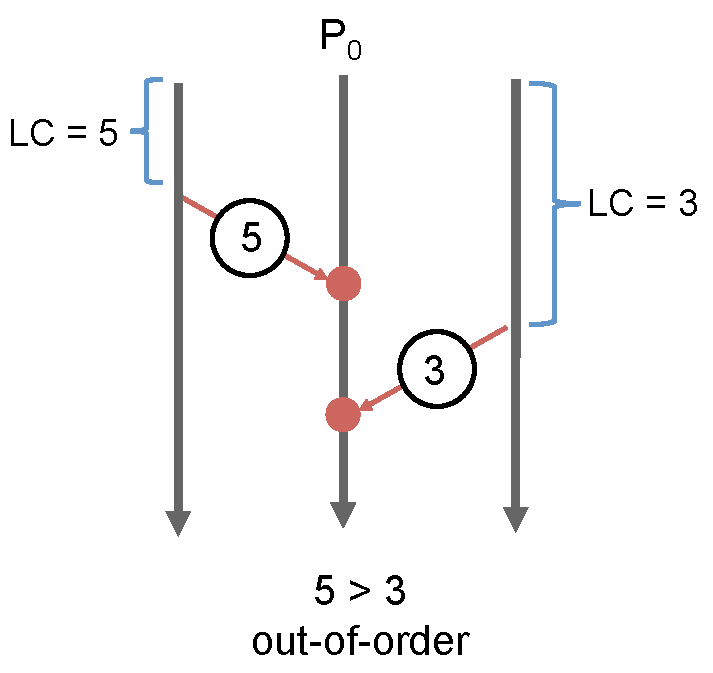
\includegraphics[width=\linewidth]{chapter_3_figures/ticking_mpisend.pdf}}
        \\ (a) Basic ticking
    \end{minipage}%
    \begin{minipage}{0.33\textwidth}
        \stackunder[5pt]{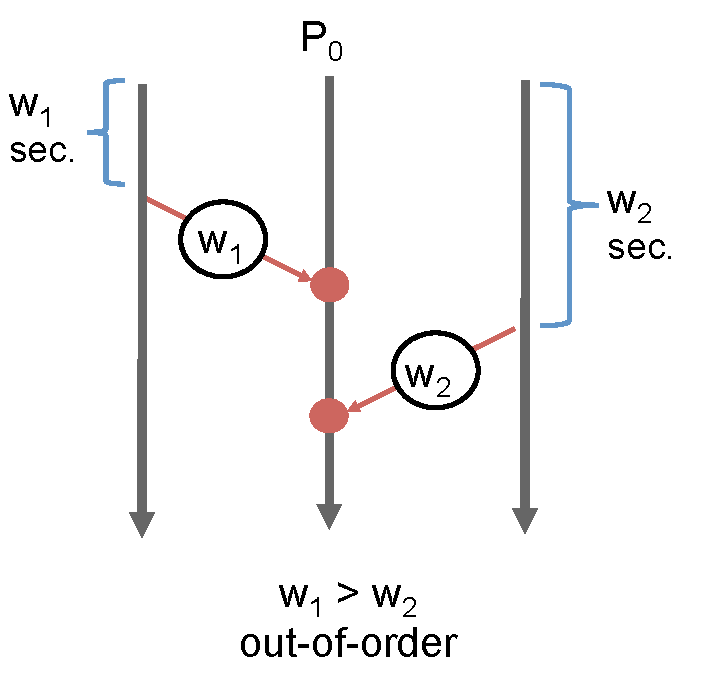
\includegraphics[width=\linewidth]{chapter_3_figures/ticking_mpiwtime.pdf}}
    \\ (b) Wall-clock ticking
    \end{minipage}%
    \begin{minipage}{0.33\textwidth}
        \stackunder[5pt]{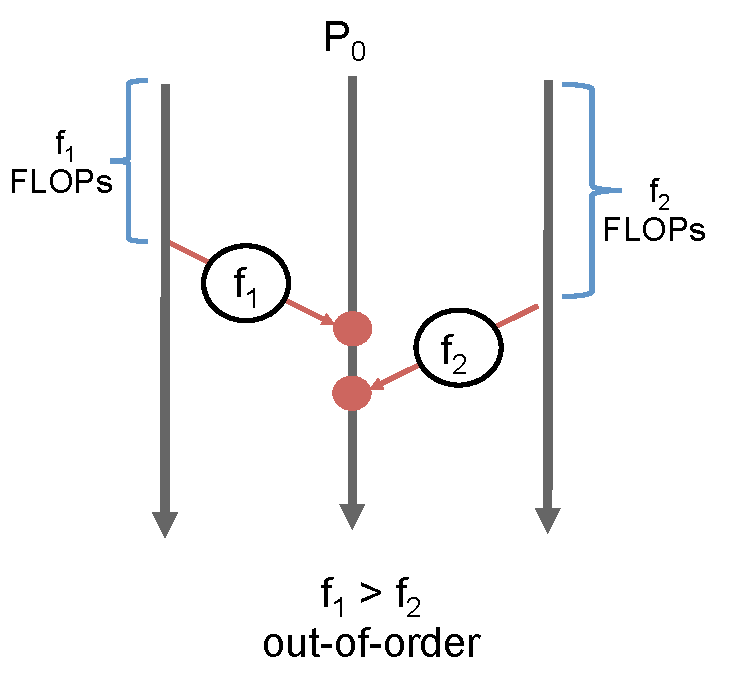
\includegraphics[width=\linewidth]{chapter_3_figures/ticking_flops.pdf}}
        \\ (c) FLOPs-based ticking
    \end{minipage}%
    \label{fig:ticking_policies}
    \caption{High level overview of the three ticking policies
      considered in this work: (a) basic ticking, (b) wall-clock
      ticking, and (c) FLOPs-based ticking.}
\end{figure}

In the message-passing HPC applications that record-and-replay tools
target, processes often alternate between progressing through
intensive floating-point workloads and communicating with other
processes. As such, we propose a FLOPs-based ticking that uses the
number of floating-point instructions completed by a process as a
proxy for wall-time. We use the Performance Application Programming
Interface (PAPI) to monitor floating-point instructions completed, and
derive ticks from those values.  Empirical investigation not shown in
this thesis indicates that the PAPI\_FP\_INS performance counter,
which measures floating-point instructions completed, yields
deterministic values, and hence deterministic ticks, when limited to
counting floating-point instructions at the application level
exclusively.  We use the MPI profiling interface (PMPI) to intercept
MPI function calls made by applications and halt PAPI's counters until
control returns to the application, as shown in
Figure~\ref{fig:ticking_policies}.(c).
 
\section{Applicability to Real Applications with Real Record-and-Replay Tool}

To evaluate the effectiveness of our PAPI\_FP\_INS-based ticking
policy in reducing the rate of out-of-order message receives, we
record multiple executions of a representative message-passing
application, the Monte Carlo Benchmark (MCB)~\cite{Software:MCB}, with a
record-and-replay tool that implements CDC, called Reproducible MPI
(ReMPI)~\cite{ClockDeltaCompression:Sato:2015}. 
In this section, we provide our rationale for
evaluating our ticking policy using MCB and ReMPI.

MCB is an MPI application that simulates particle dynamics in a domain
that is decomposed over a set of MPI processes. Particles that exit
one process's subdomain are buffered and subsequently sent to a
neighbor process's subdomain via non-blocking point-to-point
communication. MCB progresses its simulation by alternating between
three distinct communication patterns, as shown in
Figure~\ref{fig:mcb_comm_patterns}. The three patterns are:
neighbor-to-neighbor particle exchange where processes communicate
with their neighbors in a Cartesian grid; non-blocking gather where
processes are organized into a binary tree topology and send messages
to their parents in the tree; and non-blocking scatter where processes
are once again organized as a binary tree, but the direction of
communication is from parent to child.
\begin{figure}
    \centering
    \begin{minipage}{0.33\textwidth}
        \centering
        \includegraphics[width=0.9\linewidth]{chapter_3_figures/pattern_n2n}
        \\ (a) \\
    \end{minipage}% 
    \begin{minipage}{0.33\textwidth}
        \centering
        \includegraphics[width=0.9\linewidth]{chapter_3_figures/pattern_nbgather}
        \\ (b) \\
    \end{minipage}%
    \begin{minipage}{0.33\textwidth}
        \centering
        \includegraphics[width=0.9\linewidth]{chapter_3_figures/pattern_nbscatter}
         \\ (c) \\
    \end{minipage}%
    \caption{MCB communication patterns: the neighbor-to-neighbor
      particle exchange (a), the non-blocking gather (b), and the
      non-blocking scatter (c).}
    \label{fig:mcb_comm_patterns}
\end{figure}
MCB is known to exhibit non-deterministic communication due to its use
of non-blocking point-to-point communication and wildcard receives
(i.e., allowing a pending receive request to match with the first
message that arrives), rather than a message from a specific
sender. Moreover, run-to-run variability in MCB's numerical outputs
has been observed~\cite{Reproducibility:Cleveland:2013} that is
attributable to non-deterministic communication. Consequently, MCB is
an ideal candidate application for testing a record-and-replay tool.

We implement our ticking policies in ReMPI. ReMPI is, to the best
of our knowledge, the only record-and-replay tool that implements
CDC. Additionally, ReMPI's design as a composition of PMPI
modules~\cite{PMPI:Dongarra:1995}~\cite{PNMPI:Schulz:2007} simplified
the implementation of our ticking policy. By default ReMPI uses
the basic ticking policy where all ticks are set to $1$.

\section{Assessing Different Ticking Policies}

We compare our ticking policy based on floating-point operations
against the baseline ReMPI ticking policy. In our analysis we consider
the effect of application-level parameters (i.e., floating-point
workload per process and rate of messaging between processes) on the
rate of out-of-order messages.

\subsection{Experimental Setting}

By varying the number of particles that each MPI process initially
simulates, we can effectively vary the intensity of each process's
floating-point workload (i.e., the more particles are simulated per
process, the more floating point operation are performed). Note that
we consider a homogeneous distributed of particles per process. By
varying the size of the communication buffer between two processes
each process uses to accumulate particles en-route to a neighbor
process, we can effectively vary the rate of communication (i.e., by
decreasing the buffer size we increase the number of messages
issued). In Figure~\ref{fig:parameter_matrix} we show the four
scenarios we test in this thesis (in green). We consider either 1K or
1M particles for process and either a buffer size containing data for
5 or for 5,000 particles leaving a process subdomain for the neighbor
process sharing the buffer.
\begin{figure}[!ht]
    \centering
    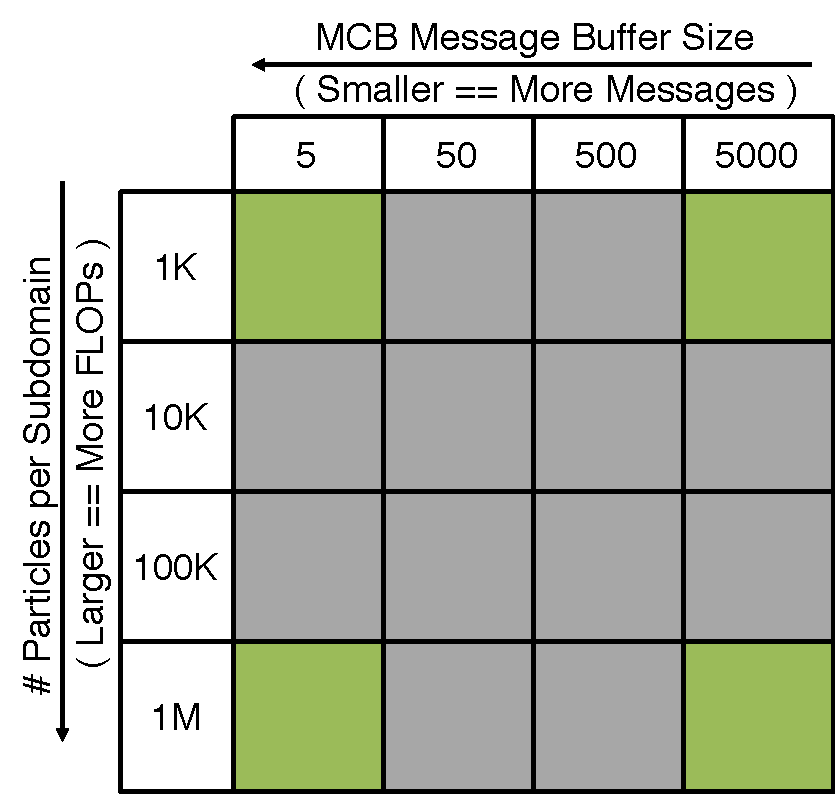
\includegraphics[width=0.5\linewidth]{chapter_3_figures/parameter_matrix.pdf}
    \caption{Tested scenarios (in green cells) in the space of
      application parameters considered in this thesis. Gray cells are
      left for future work.}
    \label{fig:parameter_matrix}
\end{figure}

For each one of the four MCB scenarios we evaluate our FLOPs-based
ticking (referred in the figures in the next section as
PAPI\_FP\_INS-ticking) against the baseline ticking policy built into
ReMPI (hereafter referred to as MPI\_SEND-ticking) and a
non-replayable wall-time-based ticking policy (referred to as
MPI\_WTIME-ticking). For each scenario and each ticking policy, we
record $100$ executions of MCB with the extended ReMPI set to log the
number of messages received in-order and the number of messages
received out-of-order by each MPI process. For each process, we
compute the percentage of messages received out-of-order, and then
aggregate these percentages across all $100$ executions, thereby
obtaining a global view of the ticking policies' effectiveness at
minimizing the rate of out-of-order messages.

We conduct our tests on Vulcan, a BlueGene/Q cluster at Lawrence
Livermore National Laboratory. Each node of Vulcan consists of 16 1.6
GHz PowerA2 processors and is equipped with 16 GB of RAM.  The nodes
are networked to each other in a 5D torus. We consider three scenarios
consisting of one single node running a 16-processes MCB, four nodes
running a 64-processes MCB, and 16 nodes running a 256-processes MCB.

\subsection{Results} \label{subsec:results}

Figures~\ref{fig:resutls1} plot the distributions of out-of-order
message percentages for each ticking policy and the median
out-of-order percentage for each ticking policy over all executions on
a single node of Vulcan.
\begin{figure}[!htb]
    \begin{minipage}[b]{0.5\linewidth}
        \centering
        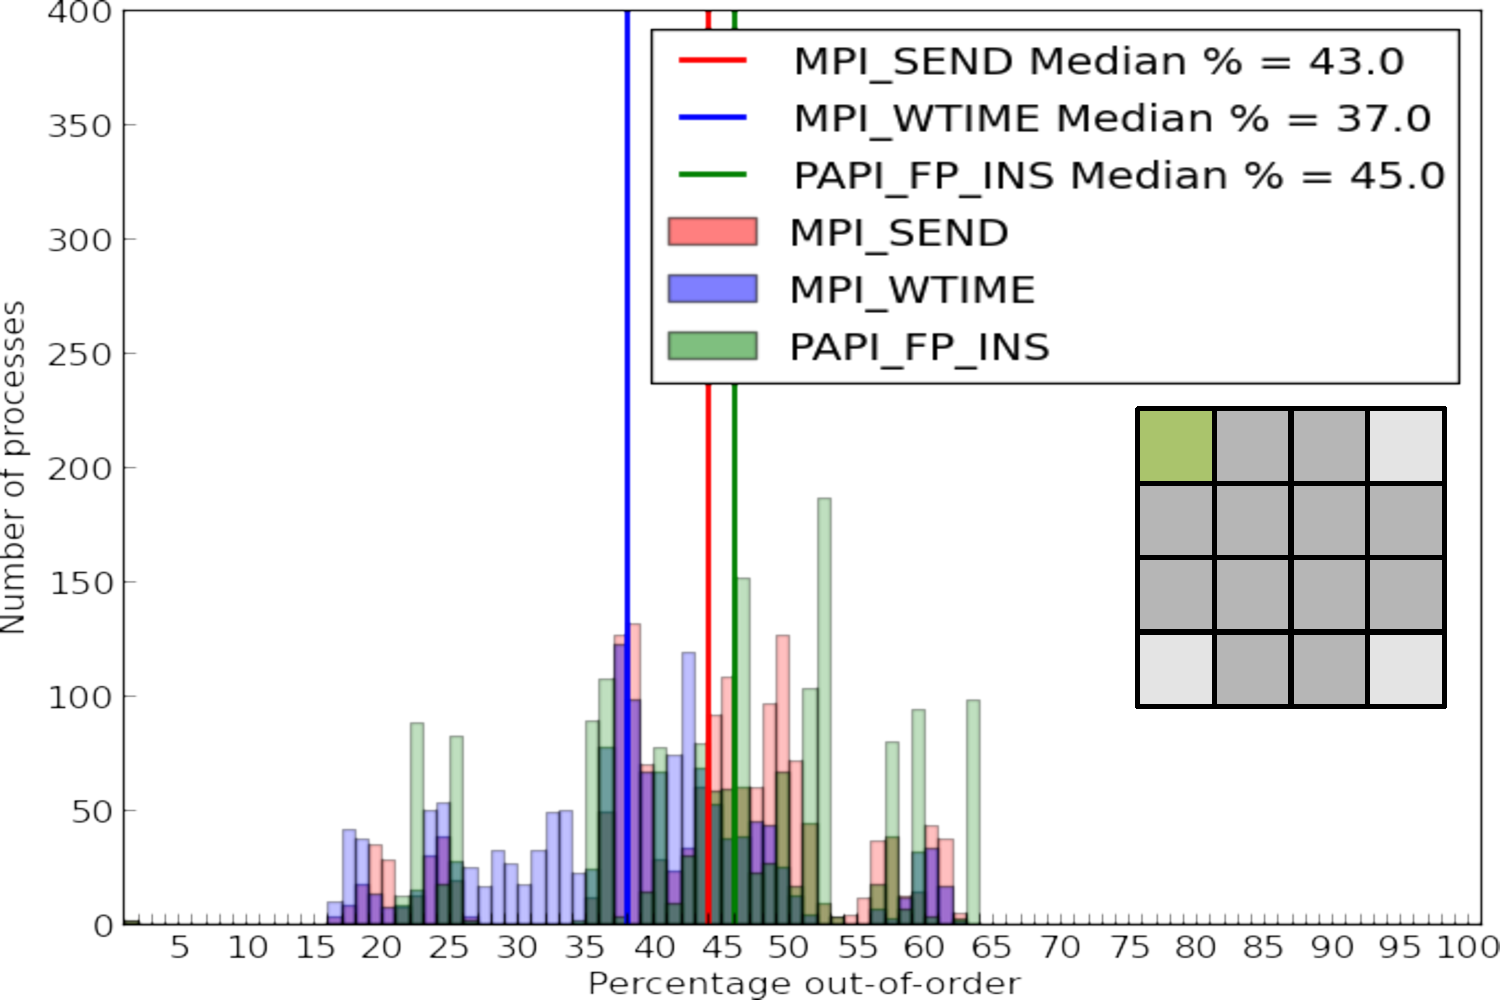
\includegraphics[width=0.95\linewidth]{chapter_3_figures/hist_nodes1_procs16_particles1000_cycles10_bufferSize5.pdf} 
        \\ (a) \\
    \end{minipage}
    \begin{minipage}[b]{0.5\linewidth}
        \centering
        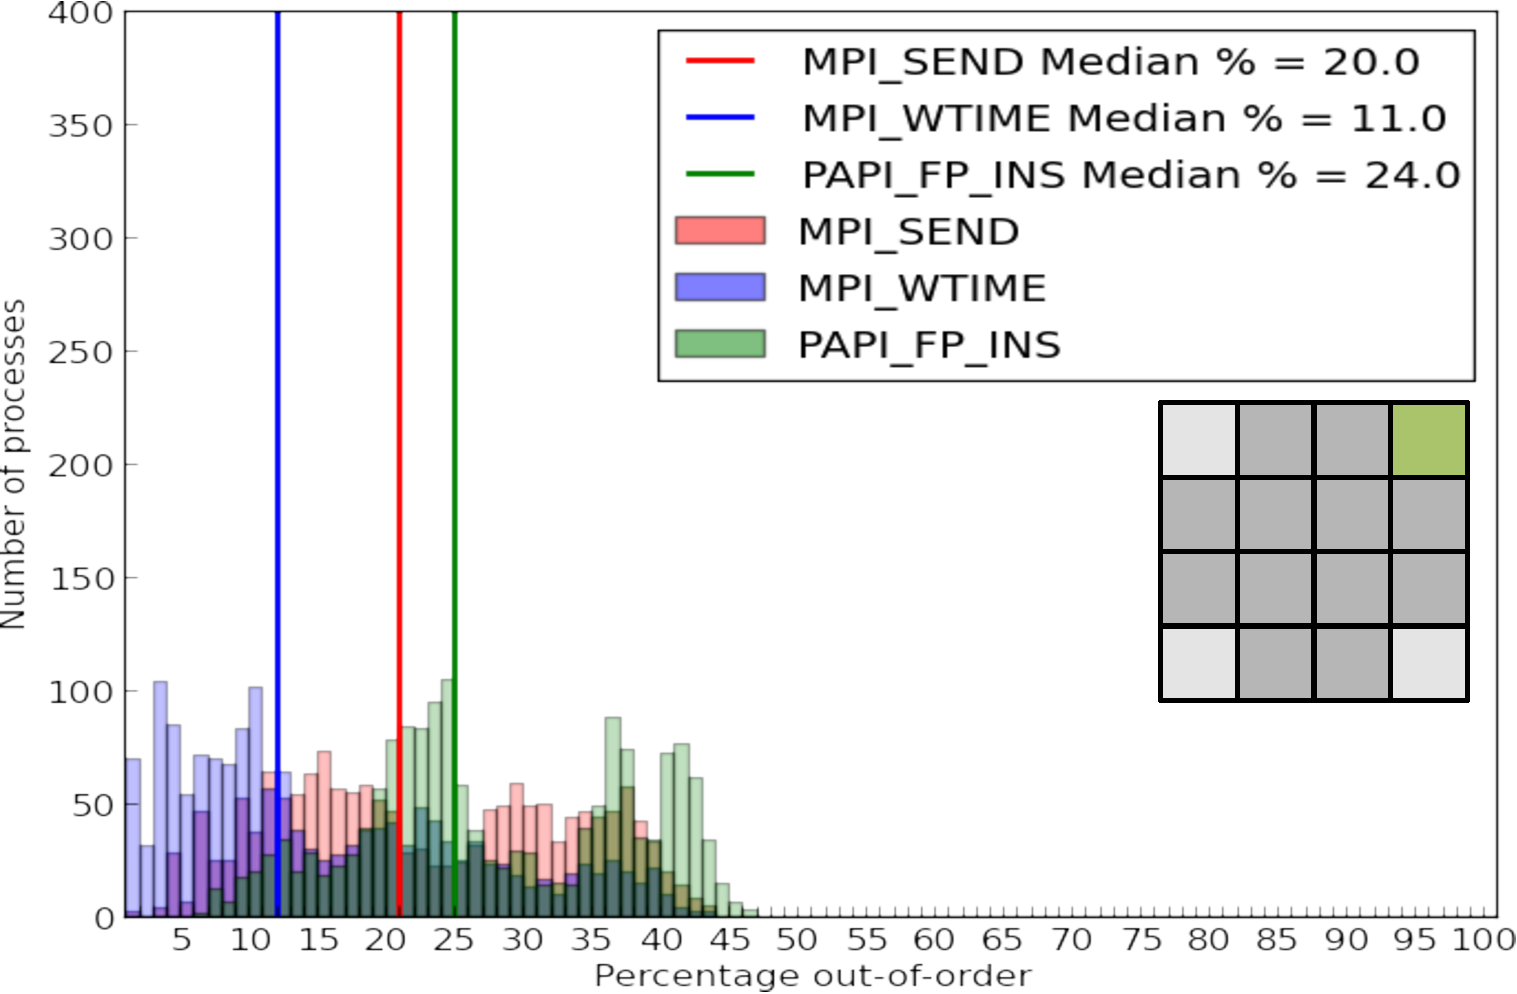
\includegraphics[width=0.95\linewidth]{chapter_3_figures/hist_nodes1_procs16_particles1000_cycles10_bufferSize5000.pdf}
        \\ (b) \\
    \end{minipage}
    \begin{minipage}[b]{0.5\linewidth}
        \centering
        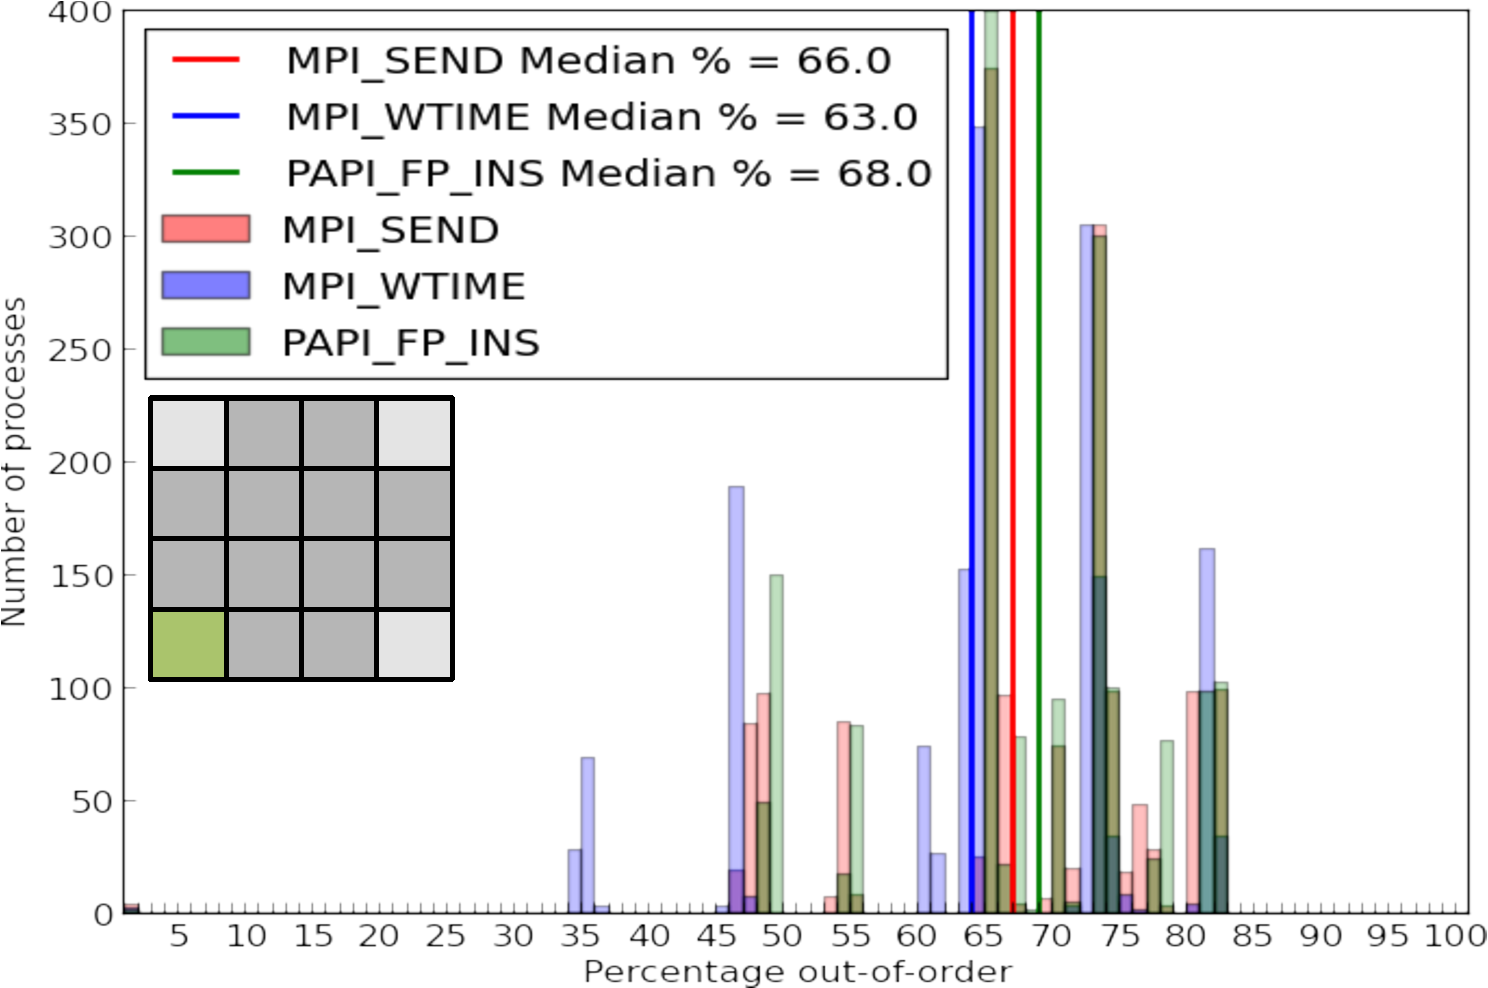
\includegraphics[width=0.95\linewidth]{chapter_3_figures/hist_nodes1_procs16_particles1000000_cycles10_bufferSize5.pdf}
        \\ (c) \\
    \end{minipage}
    \begin{minipage}[b]{0.5\linewidth}
        \centering
        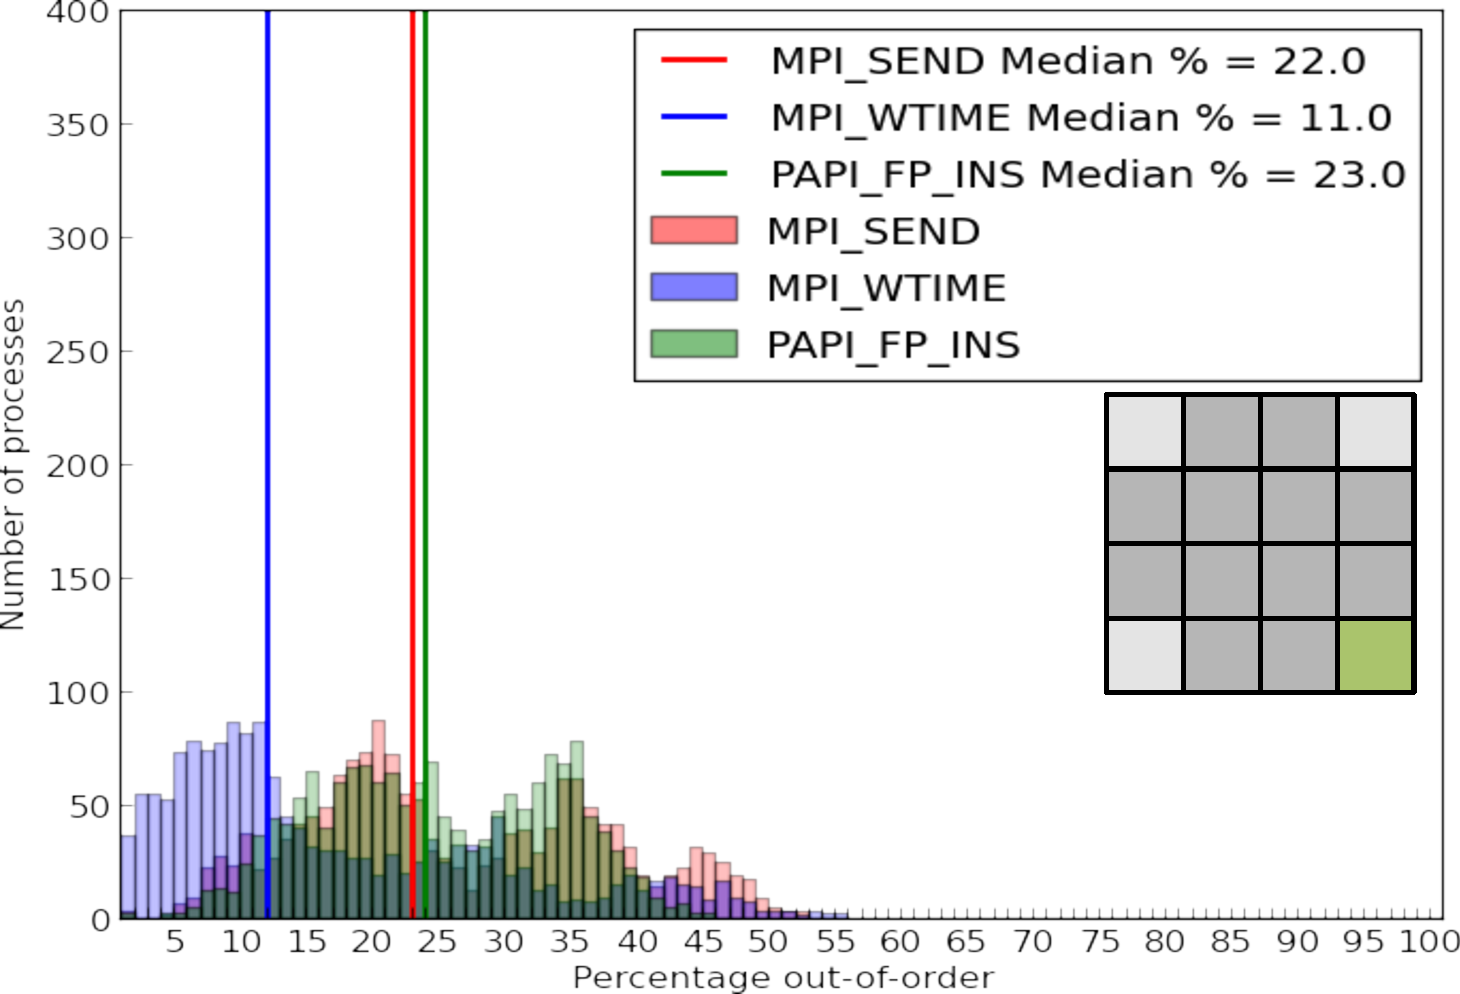
\includegraphics[width=0.95\linewidth]{chapter_3_figures/hist_nodes1_procs16_particles1000000_cycles10_bufferSize5000.pdf}
       \\ (d) \\
    \end{minipage}
    \caption{Distributions of out-of-order message percentages and
      median out-of-order percentage for each ticking policy over all
      executions on a \textbf{single node} of Vulcan. 
      The test cases are: 
      1K particles per process, buffer size 5 (a); 
      1K particles per process, buffer size 5K (b);
      1M particles per process, buffer size 5 (c);
      and 1M particles per process, buffer size 5K (d).}
    \label{fig:resutls1}
\end{figure}
At the single-node scale, we observe that MPI\_WTIME-ticking improves
the median out-of-order message percentage relative to
MPI\_SEND-ticking best when communication intensity is low (i.e., when
the MCB buffer size is large). The median improvement is $9\%$ in the
low floating-point workload case, and $11\%$ in the high
floating-point workload case. Conversely, when the communication
intensity is high due to a small MCB buffer size, the improvement
MPI\_WTIME-ticking offers is minimized--$6\%$ and $3\%$
respectively. We conjecture that this is due to the fact that when
more messages are sent per unit of wall-clock time, ticking by $1$ per
message send more closely resembles the passage of wall-clock time
than in the case where message sends are less frequent. In all four
cases however, we note that the PAPI\_FP\_INS-based ticking does not
improve the median out-of-order percentage relative to
MPI\_SEND-ticking, contrary to our expectation. We do note however
that in the low communication intensity and high floating-point
workload case, the out-of-order message rate of PAPI\_FP\_INS-ticking
closely approaches that of MPI\_SEND-ticking.

In the four-node tests shown in Figures~\ref{fig:resutls4}, we
observe that while MPI\_WTIME-ticking continues to excel in the low
communication intensity cases, MPI\_SEND-ticking matches it very
closely in the high communication intensity cases, even slightly
exceeding it when the per-process floating-point workload is also
low. Also notable is that in the two high floating-point workload
cases, PAPI\_FP\_INS-ticking matches very closely with
MPI\_SEND-ticking, lending further credence to the idea that
PAPI\_FP\_INS-ticking can be useful for applications where per-process
floating-point workload strongly influences the timing of message
sends.
\begin{figure}[!htb]
    \begin{minipage}[b]{0.5\linewidth}
        \centering
        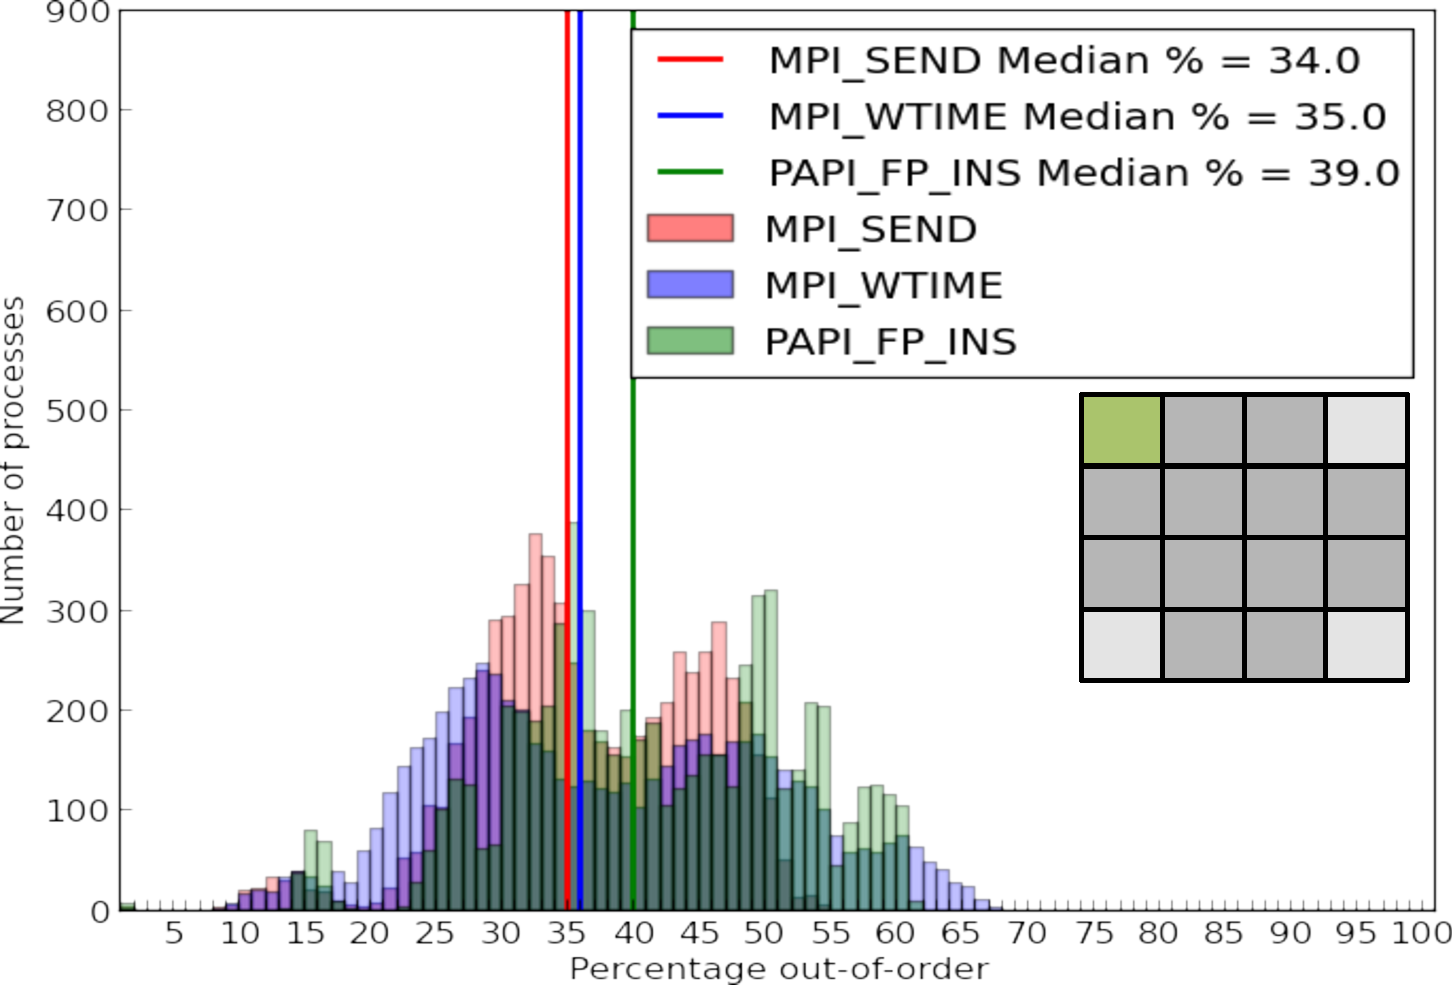
\includegraphics[width=0.95\linewidth]{chapter_3_figures/hist_nodes4_procs64_particles1000_cycles10_bufferSize5.pdf}
        \\ (a) \\
    \end{minipage}
    \begin{minipage}[b]{0.5\linewidth}
        \centering
        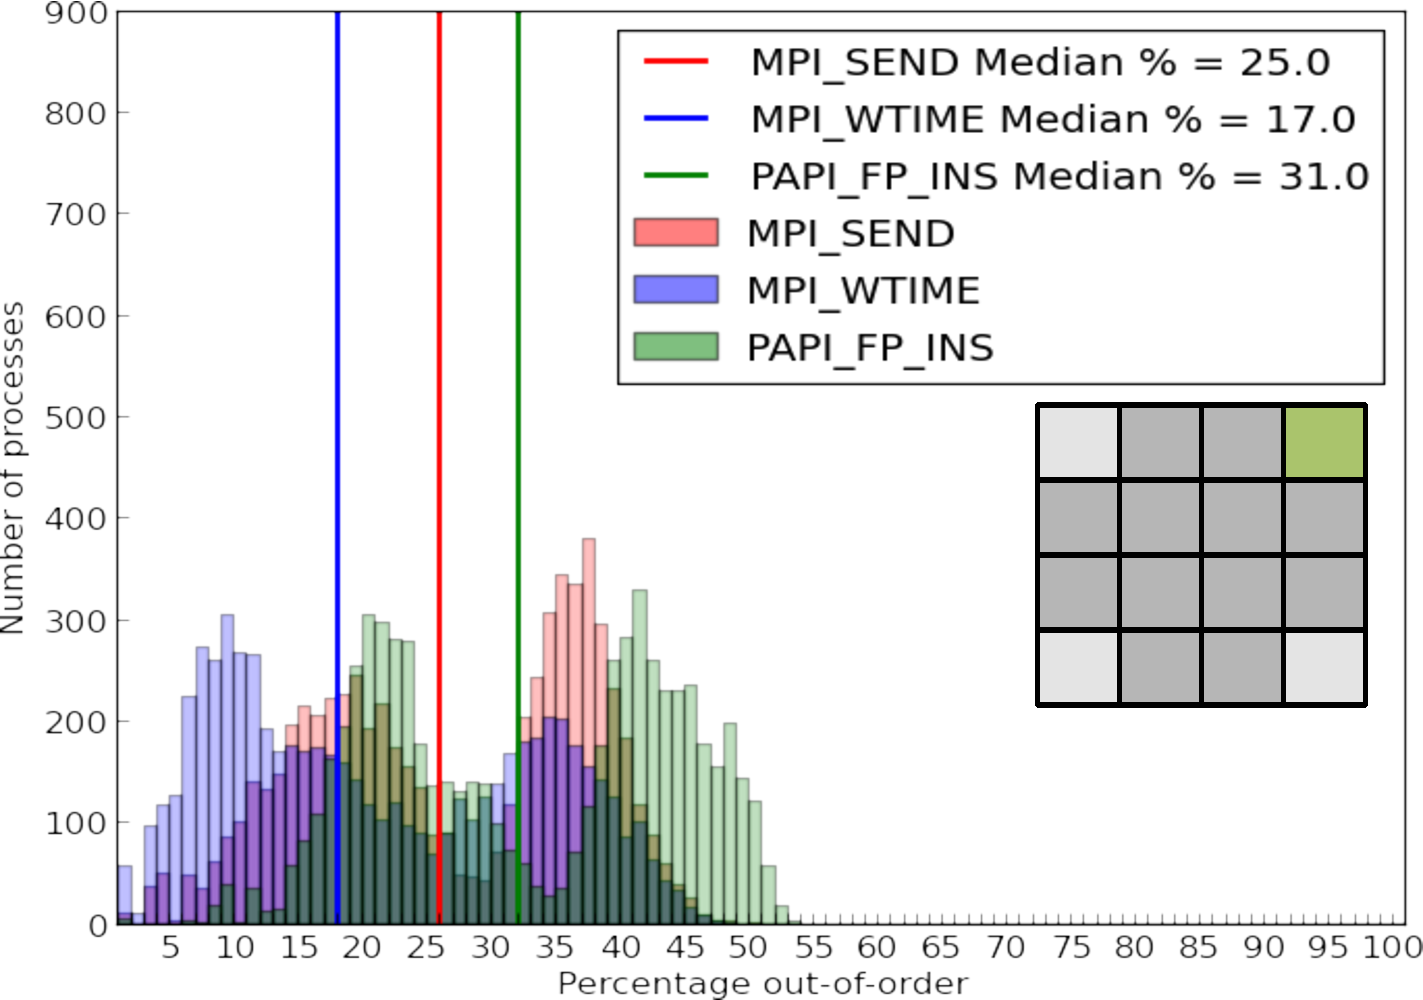
\includegraphics[width=0.95\linewidth]{chapter_3_figures/hist_nodes4_procs64_particles1000_cycles10_bufferSize5000.pdf}
        \\ (b) \\
    \end{minipage}
    \begin{minipage}[b]{0.5\linewidth}
        \centering
        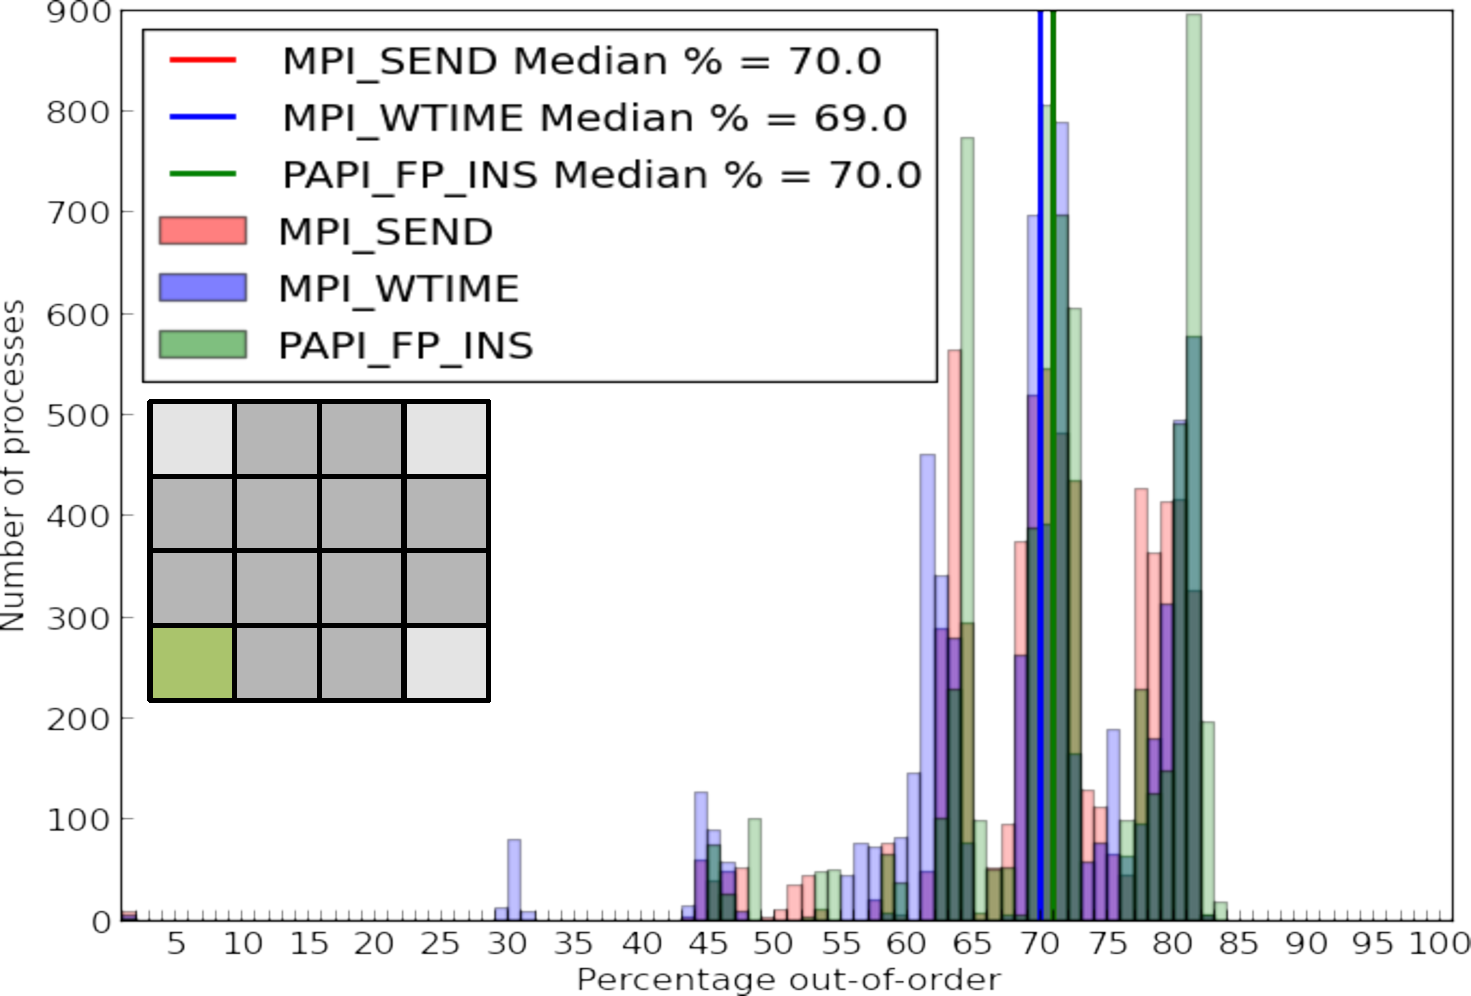
\includegraphics[width=0.95\linewidth]{chapter_3_figures/hist_nodes4_procs64_particles1000000_cycles10_bufferSize5.pdf}
        \\ (c) \\
    \end{minipage}
    \begin{minipage}[b]{0.5\linewidth}
        \centering
        \includegraphics[width=0.95\linewidth]{chapter_3_figures/hist_nodes4_procs64_particles1000000_cycles10_bufferSize5000.pdf}
       \\ (d) \\
    \end{minipage}
    \caption{Distributions of out-of-order message percentages and
      median out-of-order percentage for each ticking policy over all
      executions on \textbf{four nodes} of Vulcan.
      The test cases are: 
      1K particles per process, buffer size 5 (a); 
      1K particles per process, buffer size 5K (b);
      1M particles per process, buffer size 5 (c);
      and 1M particles per process, buffer size 5K (d).}
    \label{fig:resutls4}  
\end{figure}

At the 16-node scale shown in Figures~\ref{fig:resutls16}, we observe
that even in the low communication intensity, low floating-point
workload case, MPI\_SEND-ticking gets very close to the performance of
MPI\_WTIME-ticking. The trend we have so far observed of strong
agreement between all three ticking policies in the high communication
intensity, high floating-point workload case continues, as does the
trend of strong agreement between MPI\_SEND-ticking and
PAPI\_FP\_INS-ticking in the low communication intensity, high
floating-point workload case.
\begin{figure}[!htb]
    \begin{minipage}[b]{0.5\linewidth}
        \centering
        \includegraphics[width=0.95\linewidth]{chapter_3_figures/hist_nodes16_procs256_particles1000_cycles10_bufferSize5.pdf}
        \\ (a) \\
    \end{minipage}
    \begin{minipage}[b]{0.5\linewidth}
        \centering
        \includegraphics[width=0.95\linewidth]{chapter_3_figures/hist_nodes16_procs256_particles1000_cycles10_bufferSize5000.pdf}
        \\ (b) \\
    \end{minipage}
    \begin{minipage}[b]{0.5\linewidth}
        \centering
        \includegraphics[width=0.95\linewidth]{chapter_3_figures/hist_nodes16_procs256_particles1000000_cycles10_bufferSize5.pdf}
       \\ (c) \\
    \end{minipage}
    \begin{minipage}[b]{0.5\linewidth}
        \centering
        \includegraphics[width=0.95\linewidth]{chapter_3_figures/hist_nodes16_procs256_particles1000000_cycles10_bufferSize5000.pdf}
        \\ (d) \\
    \end{minipage}
    \caption{Distributions of out-of-order message percentages and
      median out-of-order percentage for each ticking policy over all
      executions on \textbf{16 nodes} of Vulcan.
      The test cases are: 
      1K particles per process, buffer size 5 (a); 
      1K particles per process, buffer size 5K (b);
      1M particles per process, buffer size 5 (c);
      and 1M particles per process, buffer size 5K (d).}
    \label{fig:resutls16}  
\end{figure}

\section{Lessons Learned}

The work in this chapter was motivated from the question whether a
ticking policies that resembles the non-replayable wall-clock ticking
policy such as our FLOPs-based ticking policies can outperform the
baseline ticking policy built into ReMPI. 

By comparing the performances of our 
FLOPs-based ticking against the baseline ticking policy built into
ReMPI and a non-replayable wall-time-based ticking policy in four
distinct scenarios, we have begun to develop insight into the
interaction between application behaviors and the effectiveness of
different ticking policies. Although we were not able to observe
improvement in median out-of-order percentage for the baseline
ticking policy built into our FLOPs-based ticking relative to the
baseline ticking policy built into ReMPI, we posit that our ticking
policy may still form the basis of a future ticking policy that takes
additional application-level information into account to reduce the
out-of-order message rate. Additionally, we posit that applications
exhibiting greater imbalance between processes' floating-point
workloads may benefit more from FLOPs-based ticking policies than MCB
does. 

One aspect we need to consider is that the MCB application does not
have one single communication pattern that is a source of
non-determinism, In other words, the tests we showed in this chapter
do not identify whether the out-of-order messages are more caused by one
of the three patterns. This aspect is further discussed in the next
chapter.
   

% \include{chapter_3_part_1} % ReMPI stuff
% \include{chapter_3_part_2} % ReMPI stuff

% \chapter{Conclusion and Future Work} \label{chap4}

\section{Introduction}

In this chapter, we outline the directions of our future research on
non-determinism and its impact on reproducibility of HPC applications.
So far, we have discussed the numerical challenge of reproducibility
in HPC separately from the debugging challenge; work in progress seeks
to establish connections between the two problems and their
solutions. To this end, in future work we will study connections
between run-to-run numerical variability in large scale applications
(as explored in Chapter~\ref{chap2}) and non-deterministic
communication patterns identified with record-and-replay tools (as
explored in Chapter~\ref{chap3}). The study and generalization of
non-deterministic communication patterns not only addresses
un-answered questions that were raised in the previous chapter, but
also provides a platform for identifying code motifs in applications
that lack in numerical reproducibility. We will build our work on
non-deterministic communication patterns on top of preliminary
findings from our attempts to attribute out-of-order receives to
particular communication patterns in MCB described in the next
section. The non-determinism in communication patterns cannot be
addressed without the development of better ticking policies that
mitigate the number of out-of-order events in HPC
applications. Therefore we will look at strategies to improve the
results presented in Chapter~\ref{chap3}.

\section{Out-of-Order Events and Communication Patterns}

In Chapter~\ref{chap3} we investigate the overall rate of out-of-order
messages originating from any of three communication patterns in MCB
(i.e., the neighbor-to-neighbor particle exchange, the non-blocking
gather, and the non-blocking scatter in
Figure~\ref{fig:mcb_comm_patterns}). In this section, we refine our
perspective by presenting data on the messages exchanged between
particular pairs of processes which, combined with knowledge of which
processes receive from which others during each communication pattern,
provides insight into which communication patterns are responsible for
the majority of out-of-order message receives.

To capture the specific senders of out-of-order messages to each
receiving process for each communication pattern, we instrumented the
ReMPI code to write to a log file for each received message. Note that
the log file is separate from the actual record file generated for
ReMPI use during replay. We repeated the tests described in
Figure~\ref{fig:parameter_matrix}. For each of the four cells in
Figure~\ref{fig:parameter_matrix}, we built a first heatmap with total
number of messages and a second heatmap with the total out-of-order
messages.  Specifically, in the first heatmap, for each receiving
process on the row of the heatmap, we collected the total number of
messages this process receives from each sending process on the
columns of the heatmap; the second heatmap is built in the same way
but with the number of out-of-order messages. The intensity of a
cell's coloring in the two heatmaps indicates the number of
messages. Cells colored grey indicate that no messages are
communicated between the process on the cell's row (receiving process)
and the process on the cell's column (sending process).
\begin{figure}[!htb]
    \centering
    \includegraphics[width=\linewidth]{chapter_3_figures/heatmap_interpretation}
    \caption{Interpreting a heatmap of message receives. The receiving
      processes are listed per row; the sending processes are listed
      per column.}
    \label{fig:heatmap_interpretation}
\end{figure}

Figure~\ref{fig:heatmaps_total} shows the total number of messages
received by each receiving process from each process that sent to
it. This data is collected from a 1-node, 16-process run of MCB which
was recorded using ReMPI with MPI\_SEND-ticking (the best of the two
replayable record-and replay techniques in
Chapter~\ref{chap3}. Figure~\ref{fig:heatmaps_total}.(a) refer to high
communication intensity with low floating-point workload (i.e., 1K
particles per process with a buffer size of 5);
Figure~\ref{fig:heatmaps_total}.(b) refers to low communication
intensity with low floating point workload (i.e., 1K particles per
process with a buffer size of 5K); Figure~\ref{fig:heatmaps_total}.(c)
refers to low communication intensity with high floating-point
workload (i.e., 1M particles per process, with a buffer size of 5);
and Figure~\ref{fig:heatmaps_total}.(d) refers to high communication
intensity with low floating-point workload (i.e., 1M particles per
process, with a buffer size of 5K).
\begin{figure}[ht!]
    \begin{minipage}[b]{0.5\linewidth}
        \centering
     \includegraphics[width=0.95\linewidth]{chapter_3_figures/heatmap_total_nodes1_procs16_cycles10_particles1000_bufferSize5}
        \\ (a) \\ 
    \end{minipage}%
    \begin{minipage}[b]{0.5\linewidth}
        \centering
     \includegraphics[width=0.95\linewidth]{chapter_3_figures/heatmap_total_nodes1_procs16_cycles10_particles1000_bufferSize5000}
       \\ (b) \\
    \end{minipage}
    \begin{minipage}[b]{0.5\linewidth}
        \centering
        \includegraphics[width=0.95\linewidth]{chapter_3_figures/heatmap_total_nodes1_procs16_cycles10_particles1000000_bufferSize5}
       \\ (c) \\
    \end{minipage}%
    \begin{minipage}[b]{0.5\linewidth}
        \centering
        \includegraphics[width=0.95\linewidth]{chapter_3_figures/heatmap_total_nodes1_procs16_cycles10_particles1000000_bufferSize5000}
       \\ (d) \\
    \end{minipage}
    \caption{Total number of messages received by each receiving
      process $i$ per sender process $j$ for a testcase of 1K
      particles per process, buffer size 5 (a); 1K particles per
      process, buffer size 5K (b); 1M particles per process, buffer
      size 5 (c); and 1M particles per process, buffer size 5K (d).}
    \label{fig:heatmaps_total}
\end{figure}

Figure~\ref{fig:heatmaps_out_of_order} shows heatmaps counting only
the out-of-order receives. This data is a subset of that shown in
Figure~\ref{fig:heatmaps_total} and refers to the same four
communication intensity and floating-point workload scenarios studied
above.
\begin{figure}[ht!]
    \begin{minipage}[b]{0.5\linewidth}
        \centering
        \includegraphics[width=0.95\linewidth]{chapter_3_figures/heatmap_out_of_order_nodes1_procs16_cycles10_particles1000_bufferSize5}
        \\ (a) \\
    \end{minipage}%
    \begin{minipage}[b]{0.5\linewidth}
        \centering
        \includegraphics[width=0.95\linewidth]{chapter_3_figures/heatmap_out_of_order_nodes1_procs16_cycles10_particles1000_bufferSize5000}
       \\ (b) \\
    \end{minipage}
    \begin{minipage}[b]{0.5\linewidth}
        \centering
        \includegraphics[width=0.95\linewidth]{chapter_3_figures/heatmap_out_of_order_nodes1_procs16_cycles10_particles1000000_bufferSize5}
       \\ (c) \\
    \end{minipage}%
    \begin{minipage}[b]{0.5\linewidth}
        \centering
        \includegraphics[width=0.95\linewidth]{chapter_3_figures/heatmap_out_of_order_nodes1_procs16_cycles10_particles1000000_bufferSize5000}
      \\ (d) \\ 
    \end{minipage}
    \caption{Total number of out-of-order messages received by each receiving
      process $i$ per sender process $j$ for a test case of 1K
      particles per process, buffer size 5 (a); 1K particles per
      process, buffer size 5K (b); 1M particles per process, buffer
      size 5 (c); and 1M particles per process, buffer size 5K (d).}
    \label{fig:heatmaps_out_of_order}
\end{figure}

The heatmaps with the total number of communicated message in
Figure~\ref{fig:heatmaps_total} outline how some processes only
receive from some other processes during certain communication
patterns. For example, process $P_0$ does not receive messages from
process $P_2$ during the neighbor-to-neighbor particle exchange, but
does receive messages from process $P_2$ during the nonblocking
gather. The four heatmaps in the figure confirm the three
communication patterns that we had previously extracted with the
manual inspection of the MCB code in
Figure~\ref{fig:mcb_comm_patterns}.

The inspection of the heatmaps of out-of-order messages outline which
one, if any, of the three communication patterns impacts the
non-determinism the most. In Figure~\ref{fig:heatmaps_out_of_order} we
observe that the nonblocking gather pattern is responsible for a
disproportionate amount of the out-of-order messages received. In
Figure~\ref{fig:comm_patterns_fault}, we highlight cells of the
heatmaps to indicate attribution of out-of-order receives to
particular communication patterns. Once again we observe that cells
indicating the greatest number of out-of-order receives correspond to
messages sent during the non-blocking gather communication pattern,
whereas the non-blocking scatter pattern exhibits the least.
\begin{figure}
    \centering
    %\includegraphics[width=\linewidth]{chapter_3_figures/comm_patterns_fault}
    \begin{minipage}[b]{0.33\linewidth}
        \centering
        \includegraphics[width=0.9\linewidth]{chapter_4_figures/partial_heatmap_total_gather}
    \end{minipage}%
    \begin{minipage}[b]{0.33\linewidth}
        \centering
        \includegraphics[width=\linewidth]{chapter_4_figures/comm_pattern_gather}
    \end{minipage}%
    \begin{minipage}[b]{0.33\linewidth}
        \centering
        \includegraphics[width=0.9\linewidth]{chapter_4_figures/partial_heatmap_out_of_order_gather}
    \end{minipage}
    \\
    \begin{minipage}[b]{0.33\linewidth}
        \centering
        \includegraphics[width=0.9\linewidth]{chapter_4_figures/partial_heatmap_total_n2n}
    \end{minipage}%
    \begin{minipage}[b]{0.33\linewidth}
        \centering
        \includegraphics[width=\linewidth]{chapter_4_figures/comm_pattern_n2n}
    \end{minipage}%
    \begin{minipage}[b]{0.33\linewidth}
        \centering
        \includegraphics[width=0.9\linewidth]{chapter_4_figures/partial_heatmap_out_of_order_n2n}
    \end{minipage}
    \\
    \begin{minipage}[b]{0.33\linewidth}
        \centering
        \includegraphics[width=0.9\linewidth]{chapter_4_figures/partial_heatmap_total_scatter}
        \\ (a) \\
    \end{minipage}%
    \begin{minipage}[b]{0.33\linewidth}
        \centering
        \includegraphics[width=\linewidth]{chapter_4_figures/comm_pattern_scatter}
        \\ (b) \\
    \end{minipage}%
    \begin{minipage}[b]{0.33\linewidth}
        \centering
        \includegraphics[width=0.9\linewidth]{chapter_4_figures/partial_heatmap_out_of_order_scatter}
        \\ (c) \\
    \end{minipage}
    \caption{Linking out-of-order receives to one of the three MCB
      communication patterns presented in
      Figure~\ref{fig:mcb_comm_patterns}. Because of space constraints
      only a quarter of each heatmap is shown.
      Each row shows heatmaps with receiving processes highlighted that participate in a given communication pattern.
      Column (a) shows heatmaps of total number of receives;
      column (b) shows the communication pattern;
      and column (c) shows heatmaps of the number of out-of-order receives.}
    \label{fig:comm_patterns_fault}
\end{figure}
These results are a first insight in the impact of single
communication patters on non-determinism.

\section{Adaptive Ticking Policies}

Our observation that particular out-of-order receives can be
attributed to particular communication patterns suggests a general
technique for improving a ticking policy. We propose to develop an
\textit{adaptive ticking policy} that is based on application-level
events such as floating-point instructions, but also takes into
account processes' placement in the communication topology and the
phase of communication the application is currently engaged. Our
future work in on adaptive ticking policies will proceed along two
branches.

We will first expand our investigation of communication
patterns that are found in non-deterministic HPC applications, and
enrich our understanding of how these communication patterns interact,
specifically, with ticking policies, and more generally, with record
and replay tools. We will progress this line of research by
identifying non-deterministic communication patterns in real
applications, modeling their critical characteristics, and developing
microbenchmarks based on these patterns so that their responses to
ticking policies and record-and-replay tools can be studied in
isolation. By doing so, we will systematize adaptation of tools to
applications.

Second, we will investigate the feasibility of enhancing ticking
policies such as our FLOPs-ticking with high-level information about
application behavior, such as what kind of communication pattern the
application is currently engaged in. Since we have shown that a
ticking policy that works well in one scenario (e.g., low
communication intensity and low floating-point workload) may not offer
the same benefits in another scenario, it behooves us to investigate
the feasibility of ticking policies that can adapt to application
characteristics on the fly.

%\section{Alternative Encoding of the Matched-Test Table} A
%fundamental problem that is addressed by CDC is how to represent the
%permutation that maps the observed message receive order to the
%logical clock reference order. CDC opts to represent the permutation
%by a table of indices and offsets which effectively describe the
%\textit{edits} determined by the CDC edit distance algorithm. To the
%best of our knowledge there does not exist a proof that this
%representation has minimum size for all permutations on the set of
%observed messages. Hence, we will investigate alternative encoding
%strategies for the permutations that the matched-test table must
%encode.  One alternative for representing permutations is by
%permutation ranking. Give a set of $n$ elements, it is possible to
%impose a total order on the $n!$ permutations of that set. In fact,
%one can impose one of many distinct totals orders upon that set of
%permutations. Once such a total order is imposed, one can represent a
%permutation $p$ by its rank--i.e., a single integer in the range
%$\{0, \ldots, n!\}$. While such integers, even for small $n$, can
%exceed the capacity of a 64-bit unsigned integer to represent and as
%such necessitate an arbitrary precision arithmetic library, there
%exist fast algorithms for computing the rank of a permutation
%~\cite{PermutationRanking:Myrvold:2001} and as such it may be
%worthwhile to compute permutation ranks in the event that that
%representation offers a significant reduction in size relative to the
%CDC table Another promising encoding technique for general
%permutations is proposed by Barbay and Navarro in their work on
%\textit{Left-to-Right-Minima Trees} (LRM Trees)\cite{}. This work
%describes a compressed data structure for representing permutations
%compactly that also enables a fast algorithm for application of the
%permutation, which CDC must do during replay. In particular, the
%compressed data structure enables the application of the permutation
%without decompression.

\section{Investigating Numerical Irreproducibility via Record-and-replay}

In addition to gleaning insight into how patterns of non-deterministic
communication impact the cost of applying record-and-replay techniques
such as CDC, our efforts to develop a taxonomy of non-deterministic
communication patterns will provide insight into how numerical
accuracy is impacted by non-deterministic communication. Specifically,
the ordering of receives in message-passing applications impacts
numerical reproducibility of those applications when variability in
message arrivals re-orders floating-point operands. We will explore
the use of record-and-replay tools for capturing executions exhibiting
highly accurate results, as well as those exhibiting highly inaccurate
results, in order to ascertain the internal properties of those
executions that induced, respectively, accuracy or inaccuracy.

\section{Summary}

In this thesis, we tackled the dual challenges of loss of numerical
reproducibility and loss of debuggability that non-determinism in HPC
applications presents. In response to the numerical challenge we
presented a strong case for selection of summation algorithms based on
characteristics of the floating-point operands an application is
likely deal with, and showed a quantitative comparison of compensated
summation algorithms' responses to the dynamic range and conditioning
of their inputs. 

In response to the debugging challenge, we investigated a fine-grained
logical clock ticking policy based on floating-point operations for
use in the Clock-Delta Compression record-and-replay
technique. Although our ticking policy did not provide immediate
improvements over the baseline ticking policy of CDC, we have
demonstrated the feasibility of implementing ticking policies based on
application level events, and we present preliminary findings support
further investigation into ticking policies that mold themselves to
applications' communication patterns. Finally, we propose to merge
approaches from both the numerical and debugging perspectives on
non-determinism in HPC applications in order to develop general
methodologies for addressing the reproducibility challenge.

 % Related work

\chapter{Conclusion and Future Work} \label{chap4}

\section{Introduction}

In this chapter, we outline the directions of our future research on
non-determinism and its impact on reproducibility of HPC applications.
So far, we have discussed the numerical challenge of reproducibility
in HPC separately from the debugging challenge; work in progress seeks
to establish connections between the two problems and their
solutions. To this end, in future work we will study connections
between run-to-run numerical variability in large scale applications
(as explored in Chapter~\ref{chap2}) and non-deterministic
communication patterns identified with record-and-replay tools (as
explored in Chapter~\ref{chap3}). The study and generalization of
non-deterministic communication patterns not only addresses
un-answered questions that were raised in the previous chapter, but
also provides a platform for identifying code motifs in applications
that lack in numerical reproducibility. We will build our work on
non-deterministic communication patterns on top of preliminary
findings from our attempts to attribute out-of-order receives to
particular communication patterns in MCB described in the next
section. The non-determinism in communication patterns cannot be
addressed without the development of better ticking policies that
mitigate the number of out-of-order events in HPC
applications. Therefore we will look at strategies to improve the
results presented in Chapter~\ref{chap3}.

\section{Out-of-Order Events and Communication Patterns}

In Chapter~\ref{chap3} we investigate the overall rate of out-of-order
messages originating from any of three communication patterns in MCB
(i.e., the neighbor-to-neighbor particle exchange, the non-blocking
gather, and the non-blocking scatter in
Figure~\ref{fig:mcb_comm_patterns}). In this section, we refine our
perspective by presenting data on the messages exchanged between
particular pairs of processes which, combined with knowledge of which
processes receive from which others during each communication pattern,
provides insight into which communication patterns are responsible for
the majority of out-of-order message receives.

To capture the specific senders of out-of-order messages to each
receiving process for each communication pattern, we instrumented the
ReMPI code to write to a log file for each received message. Note that
the log file is separate from the actual record file generated for
ReMPI use during replay. We repeated the tests described in
Figure~\ref{fig:parameter_matrix}. For each of the four cells in
Figure~\ref{fig:parameter_matrix}, we built a first heatmap with total
number of messages and a second heatmap with the total out-of-order
messages.  Specifically, in the first heatmap, for each receiving
process on the row of the heatmap, we collected the total number of
messages this process receives from each sending process on the
columns of the heatmap; the second heatmap is built in the same way
but with the number of out-of-order messages. The intensity of a
cell's coloring in the two heatmaps indicates the number of
messages. Cells colored grey indicate that no messages are
communicated between the process on the cell's row (receiving process)
and the process on the cell's column (sending process).
\begin{figure}[!htb]
    \centering
    \includegraphics[width=\linewidth]{chapter_3_figures/heatmap_interpretation}
    \caption{Interpreting a heatmap of message receives. The receiving
      processes are listed per row; the sending processes are listed
      per column.}
    \label{fig:heatmap_interpretation}
\end{figure}

Figure~\ref{fig:heatmaps_total} shows the total number of messages
received by each receiving process from each process that sent to
it. This data is collected from a 1-node, 16-process run of MCB which
was recorded using ReMPI with MPI\_SEND-ticking (the best of the two
replayable record-and replay techniques in
Chapter~\ref{chap3}. Figure~\ref{fig:heatmaps_total}.(a) refer to high
communication intensity with low floating-point workload (i.e., 1K
particles per process with a buffer size of 5);
Figure~\ref{fig:heatmaps_total}.(b) refers to low communication
intensity with low floating point workload (i.e., 1K particles per
process with a buffer size of 5K); Figure~\ref{fig:heatmaps_total}.(c)
refers to low communication intensity with high floating-point
workload (i.e., 1M particles per process, with a buffer size of 5);
and Figure~\ref{fig:heatmaps_total}.(d) refers to high communication
intensity with low floating-point workload (i.e., 1M particles per
process, with a buffer size of 5K).
\begin{figure}[ht!]
    \begin{minipage}[b]{0.5\linewidth}
        \centering
     \includegraphics[width=0.95\linewidth]{chapter_3_figures/heatmap_total_nodes1_procs16_cycles10_particles1000_bufferSize5}
        \\ (a) \\ 
    \end{minipage}%
    \begin{minipage}[b]{0.5\linewidth}
        \centering
     \includegraphics[width=0.95\linewidth]{chapter_3_figures/heatmap_total_nodes1_procs16_cycles10_particles1000_bufferSize5000}
       \\ (b) \\
    \end{minipage}
    \begin{minipage}[b]{0.5\linewidth}
        \centering
        \includegraphics[width=0.95\linewidth]{chapter_3_figures/heatmap_total_nodes1_procs16_cycles10_particles1000000_bufferSize5}
       \\ (c) \\
    \end{minipage}%
    \begin{minipage}[b]{0.5\linewidth}
        \centering
        \includegraphics[width=0.95\linewidth]{chapter_3_figures/heatmap_total_nodes1_procs16_cycles10_particles1000000_bufferSize5000}
       \\ (d) \\
    \end{minipage}
    \caption{Total number of messages received by each receiving
      process $i$ per sender process $j$ for a testcase of 1K
      particles per process, buffer size 5 (a); 1K particles per
      process, buffer size 5K (b); 1M particles per process, buffer
      size 5 (c); and 1M particles per process, buffer size 5K (d).}
    \label{fig:heatmaps_total}
\end{figure}

Figure~\ref{fig:heatmaps_out_of_order} shows heatmaps counting only
the out-of-order receives. This data is a subset of that shown in
Figure~\ref{fig:heatmaps_total} and refers to the same four
communication intensity and floating-point workload scenarios studied
above.
\begin{figure}[ht!]
    \begin{minipage}[b]{0.5\linewidth}
        \centering
        \includegraphics[width=0.95\linewidth]{chapter_3_figures/heatmap_out_of_order_nodes1_procs16_cycles10_particles1000_bufferSize5}
        \\ (a) \\
    \end{minipage}%
    \begin{minipage}[b]{0.5\linewidth}
        \centering
        \includegraphics[width=0.95\linewidth]{chapter_3_figures/heatmap_out_of_order_nodes1_procs16_cycles10_particles1000_bufferSize5000}
       \\ (b) \\
    \end{minipage}
    \begin{minipage}[b]{0.5\linewidth}
        \centering
        \includegraphics[width=0.95\linewidth]{chapter_3_figures/heatmap_out_of_order_nodes1_procs16_cycles10_particles1000000_bufferSize5}
       \\ (c) \\
    \end{minipage}%
    \begin{minipage}[b]{0.5\linewidth}
        \centering
        \includegraphics[width=0.95\linewidth]{chapter_3_figures/heatmap_out_of_order_nodes1_procs16_cycles10_particles1000000_bufferSize5000}
      \\ (d) \\ 
    \end{minipage}
    \caption{Total number of out-of-order messages received by each receiving
      process $i$ per sender process $j$ for a test case of 1K
      particles per process, buffer size 5 (a); 1K particles per
      process, buffer size 5K (b); 1M particles per process, buffer
      size 5 (c); and 1M particles per process, buffer size 5K (d).}
    \label{fig:heatmaps_out_of_order}
\end{figure}

The heatmaps with the total number of communicated message in
Figure~\ref{fig:heatmaps_total} outline how some processes only
receive from some other processes during certain communication
patterns. For example, process $P_0$ does not receive messages from
process $P_2$ during the neighbor-to-neighbor particle exchange, but
does receive messages from process $P_2$ during the nonblocking
gather. The four heatmaps in the figure confirm the three
communication patterns that we had previously extracted with the
manual inspection of the MCB code in
Figure~\ref{fig:mcb_comm_patterns}.

The inspection of the heatmaps of out-of-order messages outline which
one, if any, of the three communication patterns impacts the
non-determinism the most. In Figure~\ref{fig:heatmaps_out_of_order} we
observe that the nonblocking gather pattern is responsible for a
disproportionate amount of the out-of-order messages received. In
Figure~\ref{fig:comm_patterns_fault}, we highlight cells of the
heatmaps to indicate attribution of out-of-order receives to
particular communication patterns. Once again we observe that cells
indicating the greatest number of out-of-order receives correspond to
messages sent during the non-blocking gather communication pattern,
whereas the non-blocking scatter pattern exhibits the least.
\begin{figure}
    \centering
    %\includegraphics[width=\linewidth]{chapter_3_figures/comm_patterns_fault}
    \begin{minipage}[b]{0.33\linewidth}
        \centering
        \includegraphics[width=0.9\linewidth]{chapter_4_figures/partial_heatmap_total_gather}
    \end{minipage}%
    \begin{minipage}[b]{0.33\linewidth}
        \centering
        \includegraphics[width=\linewidth]{chapter_4_figures/comm_pattern_gather}
    \end{minipage}%
    \begin{minipage}[b]{0.33\linewidth}
        \centering
        \includegraphics[width=0.9\linewidth]{chapter_4_figures/partial_heatmap_out_of_order_gather}
    \end{minipage}
    \\
    \begin{minipage}[b]{0.33\linewidth}
        \centering
        \includegraphics[width=0.9\linewidth]{chapter_4_figures/partial_heatmap_total_n2n}
    \end{minipage}%
    \begin{minipage}[b]{0.33\linewidth}
        \centering
        \includegraphics[width=\linewidth]{chapter_4_figures/comm_pattern_n2n}
    \end{minipage}%
    \begin{minipage}[b]{0.33\linewidth}
        \centering
        \includegraphics[width=0.9\linewidth]{chapter_4_figures/partial_heatmap_out_of_order_n2n}
    \end{minipage}
    \\
    \begin{minipage}[b]{0.33\linewidth}
        \centering
        \includegraphics[width=0.9\linewidth]{chapter_4_figures/partial_heatmap_total_scatter}
        \\ (a) \\
    \end{minipage}%
    \begin{minipage}[b]{0.33\linewidth}
        \centering
        \includegraphics[width=\linewidth]{chapter_4_figures/comm_pattern_scatter}
        \\ (b) \\
    \end{minipage}%
    \begin{minipage}[b]{0.33\linewidth}
        \centering
        \includegraphics[width=0.9\linewidth]{chapter_4_figures/partial_heatmap_out_of_order_scatter}
        \\ (c) \\
    \end{minipage}
    \caption{Linking out-of-order receives to one of the three MCB
      communication patterns presented in
      Figure~\ref{fig:mcb_comm_patterns}. Because of space constraints
      only a quarter of each heatmap is shown.
      Each row shows heatmaps with receiving processes highlighted that participate in a given communication pattern.
      Column (a) shows heatmaps of total number of receives;
      column (b) shows the communication pattern;
      and column (c) shows heatmaps of the number of out-of-order receives.}
    \label{fig:comm_patterns_fault}
\end{figure}
These results are a first insight in the impact of single
communication patters on non-determinism.

\section{Adaptive Ticking Policies}

Our observation that particular out-of-order receives can be
attributed to particular communication patterns suggests a general
technique for improving a ticking policy. We propose to develop an
\textit{adaptive ticking policy} that is based on application-level
events such as floating-point instructions, but also takes into
account processes' placement in the communication topology and the
phase of communication the application is currently engaged. Our
future work in on adaptive ticking policies will proceed along two
branches.

We will first expand our investigation of communication
patterns that are found in non-deterministic HPC applications, and
enrich our understanding of how these communication patterns interact,
specifically, with ticking policies, and more generally, with record
and replay tools. We will progress this line of research by
identifying non-deterministic communication patterns in real
applications, modeling their critical characteristics, and developing
microbenchmarks based on these patterns so that their responses to
ticking policies and record-and-replay tools can be studied in
isolation. By doing so, we will systematize adaptation of tools to
applications.

Second, we will investigate the feasibility of enhancing ticking
policies such as our FLOPs-ticking with high-level information about
application behavior, such as what kind of communication pattern the
application is currently engaged in. Since we have shown that a
ticking policy that works well in one scenario (e.g., low
communication intensity and low floating-point workload) may not offer
the same benefits in another scenario, it behooves us to investigate
the feasibility of ticking policies that can adapt to application
characteristics on the fly.

%\section{Alternative Encoding of the Matched-Test Table} A
%fundamental problem that is addressed by CDC is how to represent the
%permutation that maps the observed message receive order to the
%logical clock reference order. CDC opts to represent the permutation
%by a table of indices and offsets which effectively describe the
%\textit{edits} determined by the CDC edit distance algorithm. To the
%best of our knowledge there does not exist a proof that this
%representation has minimum size for all permutations on the set of
%observed messages. Hence, we will investigate alternative encoding
%strategies for the permutations that the matched-test table must
%encode.  One alternative for representing permutations is by
%permutation ranking. Give a set of $n$ elements, it is possible to
%impose a total order on the $n!$ permutations of that set. In fact,
%one can impose one of many distinct totals orders upon that set of
%permutations. Once such a total order is imposed, one can represent a
%permutation $p$ by its rank--i.e., a single integer in the range
%$\{0, \ldots, n!\}$. While such integers, even for small $n$, can
%exceed the capacity of a 64-bit unsigned integer to represent and as
%such necessitate an arbitrary precision arithmetic library, there
%exist fast algorithms for computing the rank of a permutation
%~\cite{PermutationRanking:Myrvold:2001} and as such it may be
%worthwhile to compute permutation ranks in the event that that
%representation offers a significant reduction in size relative to the
%CDC table Another promising encoding technique for general
%permutations is proposed by Barbay and Navarro in their work on
%\textit{Left-to-Right-Minima Trees} (LRM Trees)\cite{}. This work
%describes a compressed data structure for representing permutations
%compactly that also enables a fast algorithm for application of the
%permutation, which CDC must do during replay. In particular, the
%compressed data structure enables the application of the permutation
%without decompression.

\section{Investigating Numerical Irreproducibility via Record-and-replay}

In addition to gleaning insight into how patterns of non-deterministic
communication impact the cost of applying record-and-replay techniques
such as CDC, our efforts to develop a taxonomy of non-deterministic
communication patterns will provide insight into how numerical
accuracy is impacted by non-deterministic communication. Specifically,
the ordering of receives in message-passing applications impacts
numerical reproducibility of those applications when variability in
message arrivals re-orders floating-point operands. We will explore
the use of record-and-replay tools for capturing executions exhibiting
highly accurate results, as well as those exhibiting highly inaccurate
results, in order to ascertain the internal properties of those
executions that induced, respectively, accuracy or inaccuracy.

\section{Summary}

In this thesis, we tackled the dual challenges of loss of numerical
reproducibility and loss of debuggability that non-determinism in HPC
applications presents. In response to the numerical challenge we
presented a strong case for selection of summation algorithms based on
characteristics of the floating-point operands an application is
likely deal with, and showed a quantitative comparison of compensated
summation algorithms' responses to the dynamic range and conditioning
of their inputs. 

In response to the debugging challenge, we investigated a fine-grained
logical clock ticking policy based on floating-point operations for
use in the Clock-Delta Compression record-and-replay
technique. Although our ticking policy did not provide immediate
improvements over the baseline ticking policy of CDC, we have
demonstrated the feasibility of implementing ticking policies based on
application level events, and we present preliminary findings support
further investigation into ticking policies that mold themselves to
applications' communication patterns. Finally, we propose to merge
approaches from both the numerical and debugging perspectives on
non-determinism in HPC applications in order to develop general
methodologies for addressing the reproducibility challenge.

 % Conclusions and future work
%\include{ref}      % This file (ref.tex) contains the text
                   % for the references.
                   
%\include{bib}      % This file (bib.tex) contains the text
                   % for a bibliography.
                                      
%
% This is the Bibliography file (bibtex.tex)
% This generally works for BibTeX

% Use sample.bib for BibTeX database
\bibliography{bibliography}
% BibTeX style (plain, alpha, unsrt)
\bibliographystyle{plain}
	 % This file (bibtex.tex) contains the text
                   % for a bibliography if using BibTeX with
                   % sample.bib
                                      
%\include{app}      % This file (app.tex) contains the text
                   % for one Appendix. 
                   
%\include{appA}     % This file (appA.tex) contains the text
                   % for Appendix A. 
                   
%\include{appB}     % This file (appB.tex) contains the text
                   % for Appendix B.   
       
\end{document}
